\documentclass[twoside]{book}

% Packages required by doxygen
\usepackage{fixltx2e}
\usepackage{calc}
\usepackage{doxygen}
\usepackage[export]{adjustbox} % also loads graphicx
\usepackage{graphicx}
\usepackage[utf8]{inputenc}
\usepackage{makeidx}
\usepackage{multicol}
\usepackage{multirow}
\PassOptionsToPackage{warn}{textcomp}
\usepackage{textcomp}
\usepackage[nointegrals]{wasysym}
\usepackage[table]{xcolor}

% Font selection
\usepackage[T1]{fontenc}
\usepackage[scaled=.90]{helvet}
\usepackage{courier}
\usepackage{amssymb}
\usepackage{sectsty}
\renewcommand{\familydefault}{\sfdefault}
\allsectionsfont{%
  \fontseries{bc}\selectfont%
  \color{darkgray}%
}
\renewcommand{\DoxyLabelFont}{%
  \fontseries{bc}\selectfont%
  \color{darkgray}%
}
\newcommand{\+}{\discretionary{\mbox{\scriptsize$\hookleftarrow$}}{}{}}

% Page & text layout
\usepackage{geometry}
\geometry{%
  a4paper,%
  top=2.5cm,%
  bottom=2.5cm,%
  left=2.5cm,%
  right=2.5cm%
}
\tolerance=750
\hfuzz=15pt
\hbadness=750
\setlength{\emergencystretch}{15pt}
\setlength{\parindent}{0cm}
\setlength{\parskip}{3ex plus 2ex minus 2ex}
\makeatletter
\renewcommand{\paragraph}{%
  \@startsection{paragraph}{4}{0ex}{-1.0ex}{1.0ex}{%
    \normalfont\normalsize\bfseries\SS@parafont%
  }%
}
\renewcommand{\subparagraph}{%
  \@startsection{subparagraph}{5}{0ex}{-1.0ex}{1.0ex}{%
    \normalfont\normalsize\bfseries\SS@subparafont%
  }%
}
\makeatother

% Headers & footers
\usepackage{fancyhdr}
\pagestyle{fancyplain}
\fancyhead[LE]{\fancyplain{}{\bfseries\thepage}}
\fancyhead[CE]{\fancyplain{}{}}
\fancyhead[RE]{\fancyplain{}{\bfseries\leftmark}}
\fancyhead[LO]{\fancyplain{}{\bfseries\rightmark}}
\fancyhead[CO]{\fancyplain{}{}}
\fancyhead[RO]{\fancyplain{}{\bfseries\thepage}}
\fancyfoot[LE]{\fancyplain{}{}}
\fancyfoot[CE]{\fancyplain{}{}}
\fancyfoot[RE]{\fancyplain{}{\bfseries\scriptsize Generated by Doxygen }}
\fancyfoot[LO]{\fancyplain{}{\bfseries\scriptsize Generated by Doxygen }}
\fancyfoot[CO]{\fancyplain{}{}}
\fancyfoot[RO]{\fancyplain{}{}}
\renewcommand{\footrulewidth}{0.4pt}
\renewcommand{\chaptermark}[1]{%
  \markboth{#1}{}%
}
\renewcommand{\sectionmark}[1]{%
  \markright{\thesection\ #1}%
}

% Indices & bibliography
\usepackage{natbib}
\usepackage[titles]{tocloft}
\setcounter{tocdepth}{3}
\setcounter{secnumdepth}{5}
\makeindex

% Hyperlinks (required, but should be loaded last)
\usepackage{ifpdf}
\ifpdf
  \usepackage[pdftex,pagebackref=true]{hyperref}
\else
  \usepackage[ps2pdf,pagebackref=true]{hyperref}
\fi
\hypersetup{%
  colorlinks=true,%
  linkcolor=blue,%
  citecolor=blue,%
  unicode%
}

% Custom commands
\newcommand{\clearemptydoublepage}{%
  \newpage{\pagestyle{empty}\cleardoublepage}%
}

\usepackage{caption}
\captionsetup{labelsep=space,justification=centering,font={bf},singlelinecheck=off,skip=4pt,position=top}

%===== C O N T E N T S =====

\begin{document}

% Titlepage & ToC
\hypersetup{pageanchor=false,
             bookmarksnumbered=true,
             pdfencoding=unicode
            }
\pagenumbering{alph}
\begin{titlepage}
\vspace*{7cm}
\begin{center}%
{\Large R\+OS Motion Planning from Scratch }\\
\vspace*{1cm}
{\large Generated by Doxygen 1.8.13}\\
\end{center}
\end{titlepage}
\clearemptydoublepage
\pagenumbering{roman}
\tableofcontents
\clearemptydoublepage
\pagenumbering{arabic}
\hypersetup{pageanchor=true}

%--- Begin generated contents ---
\chapter{Motion Planning in R\+OS from Scratch}
\label{index}\hypertarget{index}{}\subsection*{Overview}

This project is in progress.

Brief Package Descriptions\+:
\begin{DoxyItemize}
\item {\ttfamily roadmap}\+: A package with tools to generate various types of graph structured Road Maps. Currently, it supports P\+R\+Ms and Grids
\end{DoxyItemize}

Planned additions\+:
\begin{DoxyItemize}
\item Global Planning using Theta$\ast$, D$\ast$ Lite, Potential Fields
\item Local Planning with D\+WA and M\+PC
\end{DoxyItemize}

See the \href{https://rencheckyoself.github.io/motion-planning-in-ROS/}{\tt Full A\+PI} for more info.

\subsection*{How to use}

\subsubsection*{Probabilistic Road Maps}

To generate a P\+RM launch {\ttfamily roadmap view\+\_\+prm.\+launch}. This will create a new P\+RM and visualize it in Rviz.


\begin{DoxyItemize}
\item Change the parameters in {\ttfamily roadmap/config/map\+\_\+params.\+yaml} to customize the components of the map.
\end{DoxyItemize}

The following image was taken using a cell size of 0.\+2m with a buffer radius of 0.\+15m. The graph consists of 500 nodes trying to connect to the 10 nearest neighbors.



\subsubsection*{Grids}

To generate a grid, launch {\ttfamily roadmap view\+\_\+grid.\+launch}. This will create a new grid and visualize it in Rviz.


\begin{DoxyItemize}
\item Change the parameters in {\ttfamily roadmap/config/map\+\_\+params.\+yaml} to customize the components of the map.
\end{DoxyItemize}

The following image was taken using a cell size of 0.\+2m with a buffer radius of 0.\+15m. The grid has a 5 times finer resolution than the provided map, with black cells as the actual obstacle, gray cells representing cells inside the buffer zone, and white representing the free space.



\subsubsection*{Heuristic Search on a Known Map (A$\ast$ and Theta$\ast$)}

To view the algorithm in action, launch {\ttfamily global\+\_\+search plan\+\_\+prm.\+launch}. This will create a P\+RM graph, apply A$\ast$ and Theta$\ast$ search to it, and visualize the results it in Rviz.


\begin{DoxyItemize}
\item Change the parameters in {\ttfamily roadmap/config/map\+\_\+params.\+yaml} to customize the components of the map.
\item Change the parameters in {\ttfamily global\+\_\+search/config/search\+\_\+params.\+yaml} to change the start and goal locations.
\end{DoxyItemize}

The following image was taken using a cell size of 0.\+2m with a buffer radius of 0.\+15m. The graph consists of 500 nodes trying to connect to the 10 nearest neighbors. The green node is the start and the red node is the goal. The black line is the path determined by A$\ast$ and the orange line is the path determined by Theta$\ast$.



\subsubsection*{Iterative Search on an Unknown Map (L\+P\+A$\ast$ and D$\ast$ Lite)}

To view the L\+P\+A$\ast$ algorithm, launch {\ttfamily global\+\_\+search lpastar\+\_\+grid.\+launch}. This will create 2 grids, one using the stored obstacle data and one only accounting for the map boundary. L\+P\+A$\ast$ is provided the empty grid and will plan an initial path between the start and goal locations. The known grid will be used to simulate a camera or some other sensor detecting a change in the environment, which will trigger L\+P\+A$\ast$ to replan given the new information.


\begin{DoxyItemize}
\item Change the parameters in {\ttfamily roadmap/config/map\+\_\+params.\+yaml} to customize the components of the map.
\item Change the parameters in {\ttfamily global\+\_\+search/config/search\+\_\+params.\+yaml} to change the start and goal locations.
\end{DoxyItemize}

The following gif was taken using a cell size of 0.\+2m with a buffer radius of 0.\+15m and a grid resolution of 1. The green node is the start and the red node is the goal, with the black line showing the final path determined by L\+P\+A$\ast$ for the current map data. The faded area of the map is assumed by the search to be completely free and occupancy data is filled in one row at a time from the bottom up. Cells marked with a light blue square indicate that it was updated during the most recent search.



To view the D$\ast$ Lite algorithm, launch {\ttfamily global\+\_\+search dstarlite\+\_\+grid.\+launch}. This will create 2 grids, one using the stored obstacle data and one only accounting for the map boundary. D$\ast$ Lite is provided the empty grid and will plan an initial path between the start and goal locations. The known grid will be used to simulate a sensor mounted to the robot to detect a change in the environment within a given radius around the robot. This will trigger D$\ast$ Lite to replan given the new information.


\begin{DoxyItemize}
\item Change the parameters in {\ttfamily roadmap/config/map\+\_\+params.\+yaml} to customize the components of the map.
\item Change the parameters in {\ttfamily global\+\_\+search/config/search\+\_\+params.\+yaml} to change the start and goal locations and the sensor range.
\end{DoxyItemize}

The following gif was taken using a cell size of 0.\+2m with a buffer radius of 0.\+15m, a grid resolution of 1, and a simulated sensor range of 0.\+6m. The green node is the start and the red node is the goal and the robot is the blue cube. The black line represents the path the robot has taken and the orange line is the path determined by D$\ast$ Lite for the current map data. The faded area of the map is assumed by the search to be completely free and occupancy data is filled as the simulated sensor is able to detect the cell. Cells marked with a light blue square indicate that it was updated during the most recent search.



\subsubsection*{Potential Fields}

To view the algorithm in action, launch {\ttfamily global\+\_\+search plan\+\_\+potential\+\_\+fields.\+launch}. This will use the existing map data to plan a path from start to goal using the standard potential field algorithm. This implementation does not currently provide a means of escaping local minima and assumes a fully known map.


\begin{DoxyItemize}
\item Change the parameters in {\ttfamily roadmap/config/map\+\_\+params.\+yaml} to customize the components of the map.
\item Change the parameters in {\ttfamily global\+\_\+search/config/search\+\_\+params.\+yaml} to change the start and goal locations and potential field parameters.
\end{DoxyItemize}

The following gif was taken using a cell size of 0.\+2 with the following potential field parameters\+: 
\begin{DoxyCode}
att\_weight: 0.6 # weighting factor the attactive component
dgstar: 3 # piecewise threshold for attractive gradient
rep\_weight: 0.1 # weighting factor the repulsive component
Qstar: 0.4 # obstacle range of influence
epsilon: 0.05 # termination threshold
zeta: 0.01 # step size
\end{DoxyCode}
 The green node is the start and the red node is the goal and the orange line is the path determined by the potential field algorithm.



\subsubsection*{M\+P\+PI}

To view the algorithm in action, launch {\ttfamily mppi\+\_\+control turtlebot\+\_\+mppi.\+launch}. After launching, call the {\ttfamily /start} service from the terminal to begin the waypoint following. This will apply the mppi control algorithm to calculate a control sequence to drive the robot to a series of waypoints. This package depends on a couple of packages located in my other {\ttfamily ros\+\_\+navigation\+\_\+from\+\_\+scratch} repo. Use the included .rosinstall file to ensure you get the correct packages.


\begin{DoxyItemize}
\item Change parameters in the mppi\+\_\+control/config/control\+\_\+param.\+yaml to tune the controller
\end{DoxyItemize}

This example is using M\+P\+PI control to select wheel velocities for a differential drive robot to drive through consecutive waypoints. Each waypoint is an (x,y,heading) tuple. The parameters used are shown in the configuration file. Due to the random sampling each run is slightly different, but exhibit the same general behavior.



Also included in {\ttfamily mppi\+\_\+control/testing\+\_\+files} is a python-\/only script to perform the same algorithm. To use this script, execute the {\ttfamily mppi.\+py} file. It is currently configured to have a unicycle model robot follow waypoints. Below are some results for various robots and tasks\+:

The first plot is using the unicycle kinematic model to solve the parallel parking problem. The output of the control algorithm is linear and angular velocities. See the python script for all of the parameters.



The plot below is using the differential drive kinematic model to solve the parallel parking problem. The output of the control algorithm is right and left wheel velocities. See the python script for all of the parameters.



The third plot is using the unicycle kinematic model to follow a series of waypoint. The output of the control algorithm is linear and angular velocities. See the python script for all of the parameters.



\subsection*{Background}

\subsubsection*{Probabilistic Road Map}

A P\+RM is a means to efficiently constructing a system of valid pathways through an environment as it has the advantage to plan in high dimensional configuration spaces. The assembly starts by randomly sampling states and only keeping them if they are a valid. In this implementation, a valid node is an x,y position that is not within the bounds of an obstacle or its buffer zone. After N number of valid nodes have been sampled each node is connected to it\textquotesingle{}s k-\/nearest neighbors along valid straight line paths. In this implementation a path or edge is considered valid if it does not intersect an obstacle or it\textquotesingle{}s buffer zone.

The challenging part of implementing a P\+RM is identifying how to determine if a node/edge is valid. This implementation currently only supports convex obstacles and expects that the vertices are provided in counterclockwise order. The collision detection is as follows\+:
\begin{DoxyItemize}
\item To determine if a sampled node is inside of an obstacle, test if the state is on the same side of all of the line segments.
\item To determine if a sampled node is inside the buffer zone, calculate that shortest distance to each line segment and compare it to the desired buffer distance.
\item To determine if an edge between two nodes is
\end{DoxyItemize}

\subsection*{References and Resources}


\begin{DoxyItemize}
\item La\+Valle, Steven M. Planning algorithms. Cambridge university press, 2006.
\item Choset, Howie M., et al. Principles of robot motion\+: theory, algorithms, and implementation. M\+IT press, 2005.
\item Latombe, Lydia E. Kavraki Jean-\/\+Claude. ”\+Probabilistic Roadmaps for Robot Path Planning.\+” Prati-\/ cal motion planning in robotics\+: current aproaches and future challenges (1998)\+: 33-\/53.
\item Daniel, Kenny, et al. ”\+Theta$\ast$\+: Any-\/angle path planning on grids.\+” Journal of Artificial In-\/ telligence Research 39 (2010)\+: 533-\/579.
\item Koenig, Sven, and Maxim Likhachev. ”\+Fast replanning for navigation in unknown terrain.\+” I\+E\+EE Transactions on Robotics 21.\+3 (2005)\+: 354-\/363.
\item Williams, Grady, Andrew Aldrich, and Evangelos Theodorou. \char`\"{}\+Model predictive path integral control using covariance variable importance sampling.\char`\"{} ar\+Xiv preprint ar\+Xiv\+:1509.\+01149 (2015).
\item Abraham, Ian, et al. \char`\"{}\+Model-\/\+Based Generalization Under Parameter Uncertainty Using Path Integral Control.\char`\"{} I\+E\+EE Robotics and Automation Letters 5.\+2 (2020)\+: 2864-\/2871. 
\end{DoxyItemize}
\chapter{Hierarchical Index}
\section{Class Hierarchy}
This inheritance list is sorted roughly, but not completely, alphabetically\+:\begin{DoxyCompactList}
\item \contentsline{section}{collision\+:\+:Dist\+Res}{\pageref{structcollision_1_1DistRes}}{}
\item \contentsline{section}{prm\+:\+:Edge}{\pageref{structprm_1_1Edge}}{}
\item \contentsline{section}{grid\+:\+:Grid}{\pageref{classgrid_1_1Grid}}{}
\item \contentsline{section}{hsearch\+:\+:H\+Search}{\pageref{classhsearch_1_1HSearch}}{}
\begin{DoxyCompactList}
\item \contentsline{section}{hsearch\+:\+:A\+Star}{\pageref{classhsearch_1_1AStar}}{}
\item \contentsline{section}{hsearch\+:\+:Theta\+Star}{\pageref{classhsearch_1_1ThetaStar}}{}
\end{DoxyCompactList}
\item \contentsline{section}{grid\+:\+:Map}{\pageref{structgrid_1_1Map}}{}
\item \contentsline{section}{prm\+:\+:Node}{\pageref{structprm_1_1Node}}{}
\item \contentsline{section}{prm\+:\+:Road\+Map}{\pageref{classprm_1_1RoadMap}}{}
\item \contentsline{section}{hsearch\+:\+:Search\+Node}{\pageref{structhsearch_1_1SearchNode}}{}
\end{DoxyCompactList}

\chapter{Class Index}
\section{Class List}
Here are the classes, structs, unions and interfaces with brief descriptions\+:\begin{DoxyCompactList}
\item\contentsline{section}{\hyperlink{classhsearch_1_1AStar}{hsearch\+::\+A\+Star} \\*A$\ast$ Search class derived from the \hyperlink{classhsearch_1_1HSearch}{H\+Search} class }{\pageref{classhsearch_1_1AStar}}{}
\item\contentsline{section}{\hyperlink{structcollision_1_1DistRes}{collision\+::\+Dist\+Res} \\*Used to return information from the point to line distance function }{\pageref{structcollision_1_1DistRes}}{}
\item\contentsline{section}{\hyperlink{structprm_1_1Edge}{prm\+::\+Edge} \\*A struct to fully describe a connection between two nodes }{\pageref{structprm_1_1Edge}}{}
\item\contentsline{section}{\hyperlink{classgrid_1_1Grid}{grid\+::\+Grid} \\*Class to create a \hyperlink{classgrid_1_1Grid}{Grid} overlay for provided \hyperlink{structgrid_1_1Map}{Map} information }{\pageref{classgrid_1_1Grid}}{}
\item\contentsline{section}{\hyperlink{classhsearch_1_1HSearch}{hsearch\+::\+H\+Search} \\*The base class to define a heuristic based search algorithm. This class has no Compute\+Cost funtion which is required to find the shortest path. This function is defined in the derived class to determine the type of search. Some searched also have a different flow for finding the shortest path, which is why the Compute\+Shortest\+Path method is virtual }{\pageref{classhsearch_1_1HSearch}}{}
\item\contentsline{section}{\hyperlink{structgrid_1_1Map}{grid\+::\+Map} \\*Contains information about a bound map }{\pageref{structgrid_1_1Map}}{}
\item\contentsline{section}{\hyperlink{structprm_1_1Node}{prm\+::\+Node} \\*A struct to define a node and interact with it }{\pageref{structprm_1_1Node}}{}
\item\contentsline{section}{\hyperlink{classprm_1_1RoadMap}{prm\+::\+Road\+Map} \\*A class to build a Probabilistic Road Maps based on provided Map information }{\pageref{classprm_1_1RoadMap}}{}
\item\contentsline{section}{\hyperlink{structhsearch_1_1SearchNode}{hsearch\+::\+Search\+Node} \\*Information used by a search algorithm }{\pageref{structhsearch_1_1SearchNode}}{}
\item\contentsline{section}{\hyperlink{classhsearch_1_1ThetaStar}{hsearch\+::\+Theta\+Star} \\*Theta$\ast$ any-\/angle path planner derived from the \hyperlink{classhsearch_1_1HSearch}{H\+Search} class }{\pageref{classhsearch_1_1ThetaStar}}{}
\end{DoxyCompactList}

\chapter{File Index}
\section{File List}
Here is a list of all documented files with brief descriptions\+:\begin{DoxyCompactList}
\item\contentsline{section}{roadmap/include/roadmap/\hyperlink{collision_8hpp}{collision.\+hpp} \\*A library containing functions to detect various types of collisions }{\pageref{collision_8hpp}}{}
\item\contentsline{section}{roadmap/include/roadmap/\hyperlink{grid_8hpp}{grid.\+hpp} \\*A library for building an occupancy grid }{\pageref{grid_8hpp}}{}
\item\contentsline{section}{roadmap/include/roadmap/\hyperlink{prm_8hpp}{prm.\+hpp} \\*A library for building a Probabilistic Road Map }{\pageref{prm_8hpp}}{}
\item\contentsline{section}{roadmap/include/roadmap/\hyperlink{utility_8hpp}{utility.\+hpp} \\*A library of utility functions for the various nodes and libraries of this package }{\pageref{utility_8hpp}}{}
\item\contentsline{section}{roadmap/src/\hyperlink{draw__world_8cpp}{draw\+\_\+world.\+cpp} \\*Node to draw the features of the real world map }{\pageref{draw__world_8cpp}}{}
\item\contentsline{section}{roadmap/src/\hyperlink{make__roadmap_8cpp}{make\+\_\+roadmap.\+cpp} \\*Node to create and draw a probabilistic road map }{\pageref{make__roadmap_8cpp}}{}
\item\contentsline{section}{roadmap/src/roadmap/\hyperlink{collision_8cpp}{collision.\+cpp} \\*A library containing functions to detect various types of collisions }{\pageref{collision_8cpp}}{}
\item\contentsline{section}{roadmap/src/roadmap/\hyperlink{grid_8cpp}{grid.\+cpp} \\*A library for building an occupied grid }{\pageref{grid_8cpp}}{}
\item\contentsline{section}{roadmap/src/roadmap/\hyperlink{prm_8cpp}{prm.\+cpp} \\*A library for building a Probabilistic Road Map }{\pageref{prm_8cpp}}{}
\end{DoxyCompactList}

\chapter{Class Documentation}
\hypertarget{classhsearch_1_1AStar}{}\section{hsearch\+:\+:A\+Star Class Reference}
\label{classhsearch_1_1AStar}\index{hsearch\+::\+A\+Star@{hsearch\+::\+A\+Star}}


A$\ast$ Search class derived from the \hyperlink{classhsearch_1_1HSearch}{H\+Search} class.  




{\ttfamily \#include $<$heuristic\+\_\+search.\+hpp$>$}



Inheritance diagram for hsearch\+:\+:A\+Star\+:\nopagebreak
\begin{figure}[H]
\begin{center}
\leavevmode
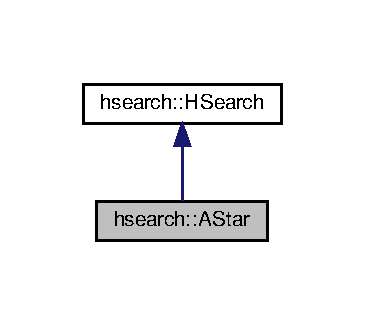
\includegraphics[width=175pt]{db/db4/classhsearch_1_1AStar__inherit__graph}
\end{center}
\end{figure}


Collaboration diagram for hsearch\+:\+:A\+Star\+:\nopagebreak
\begin{figure}[H]
\begin{center}
\leavevmode
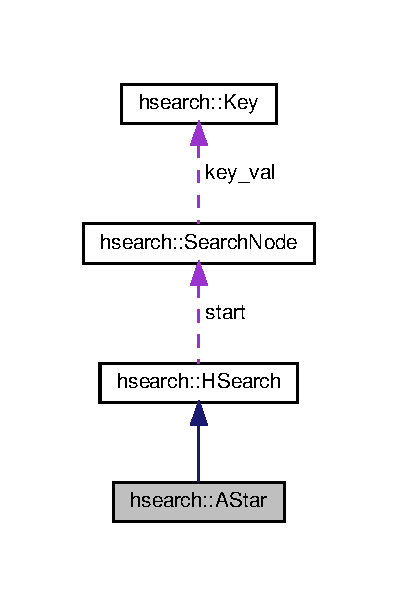
\includegraphics[width=191pt]{d6/d18/classhsearch_1_1AStar__coll__graph}
\end{center}
\end{figure}
\subsection*{Public Member Functions}
\begin{DoxyCompactItemize}
\item 
\hyperlink{classhsearch_1_1AStar_ad3897420abd92fefbd9e9270689418b8}{A\+Star} (std\+::vector$<$ \hyperlink{structprm_1_1Node}{prm\+::\+Node} $>$ $\ast$node\+\_\+list)
\begin{DoxyCompactList}\small\item\em Initialize the search with the created graph. \end{DoxyCompactList}\end{DoxyCompactItemize}
\subsection*{Protected Member Functions}
\begin{DoxyCompactItemize}
\item 
void \hyperlink{classhsearch_1_1AStar_a3a9a3c398437d9efe0b9943c29a8672b}{Compute\+Cost} (\hyperlink{structhsearch_1_1SearchNode}{Search\+Node} \&s, \hyperlink{structhsearch_1_1SearchNode}{Search\+Node} \&sp)
\begin{DoxyCompactList}\small\item\em calculates the path 1 cost between the two nodes \end{DoxyCompactList}\end{DoxyCompactItemize}
\subsection*{Additional Inherited Members}


\subsection{Detailed Description}
A$\ast$ Search class derived from the \hyperlink{classhsearch_1_1HSearch}{H\+Search} class. 

\subsection{Constructor \& Destructor Documentation}
\mbox{\Hypertarget{classhsearch_1_1AStar_ad3897420abd92fefbd9e9270689418b8}\label{classhsearch_1_1AStar_ad3897420abd92fefbd9e9270689418b8}} 
\index{hsearch\+::\+A\+Star@{hsearch\+::\+A\+Star}!A\+Star@{A\+Star}}
\index{A\+Star@{A\+Star}!hsearch\+::\+A\+Star@{hsearch\+::\+A\+Star}}
\subsubsection{\texorpdfstring{A\+Star()}{AStar()}}
{\footnotesize\ttfamily hsearch\+::\+A\+Star\+::\+A\+Star (\begin{DoxyParamCaption}\item[{std\+::vector$<$ \hyperlink{structprm_1_1Node}{prm\+::\+Node} $>$ $\ast$}]{node\+\_\+list }\end{DoxyParamCaption})\hspace{0.3cm}{\ttfamily [inline]}}



Initialize the search with the created graph. 


\begin{DoxyParams}{Parameters}
{\em node\+\_\+list} & pointer to a vector of Nodes that create a graph \\
\hline
\end{DoxyParams}


\subsection{Member Function Documentation}
\mbox{\Hypertarget{classhsearch_1_1AStar_a3a9a3c398437d9efe0b9943c29a8672b}\label{classhsearch_1_1AStar_a3a9a3c398437d9efe0b9943c29a8672b}} 
\index{hsearch\+::\+A\+Star@{hsearch\+::\+A\+Star}!Compute\+Cost@{Compute\+Cost}}
\index{Compute\+Cost@{Compute\+Cost}!hsearch\+::\+A\+Star@{hsearch\+::\+A\+Star}}
\subsubsection{\texorpdfstring{Compute\+Cost()}{ComputeCost()}}
{\footnotesize\ttfamily void hsearch\+::\+A\+Star\+::\+Compute\+Cost (\begin{DoxyParamCaption}\item[{\hyperlink{structhsearch_1_1SearchNode}{Search\+Node} \&}]{s,  }\item[{\hyperlink{structhsearch_1_1SearchNode}{Search\+Node} \&}]{sp }\end{DoxyParamCaption})\hspace{0.3cm}{\ttfamily [protected]}, {\ttfamily [virtual]}}



calculates the path 1 cost between the two nodes 


\begin{DoxyParams}{Parameters}
{\em s} & the current node being expanded \\
\hline
{\em sp} & the neighbor node being evaluated \\
\hline
\end{DoxyParams}


Implements \hyperlink{classhsearch_1_1HSearch_a5d325955c4faedaca0c68155fd1f7e69}{hsearch\+::\+H\+Search}.



The documentation for this class was generated from the following files\+:\begin{DoxyCompactItemize}
\item 
global\+\_\+search/include/global\+\_\+search/\hyperlink{heuristic__search_8hpp}{heuristic\+\_\+search.\+hpp}\item 
global\+\_\+search/src/global\+\_\+search/\hyperlink{heuristic__search_8cpp}{heuristic\+\_\+search.\+cpp}\end{DoxyCompactItemize}

\hypertarget{structcollision_1_1DistRes}{}\section{collision\+:\+:Dist\+Res Struct Reference}
\label{structcollision_1_1DistRes}\index{collision\+::\+Dist\+Res@{collision\+::\+Dist\+Res}}


Used to return information from the point to line distance function.  




{\ttfamily \#include $<$collision.\+hpp$>$}

\subsection*{Public Member Functions}
\begin{DoxyCompactItemize}
\item 
\hyperlink{structcollision_1_1DistRes_a1275e0b506edcd9aa0cdaa72a61d1ae7}{Dist\+Res} (bool status, double dist)
\begin{DoxyCompactList}\small\item\em Create the result of the point to line distance function. \end{DoxyCompactList}\end{DoxyCompactItemize}
\subsection*{Public Attributes}
\begin{DoxyCompactItemize}
\item 
\mbox{\Hypertarget{structcollision_1_1DistRes_a9da4071fdc224d798adb12dcb1cfff58}\label{structcollision_1_1DistRes_a9da4071fdc224d798adb12dcb1cfff58}} 
bool \hyperlink{structcollision_1_1DistRes_a9da4071fdc224d798adb12dcb1cfff58}{inside\+\_\+segment}
\begin{DoxyCompactList}\small\item\em True if the point lies inbetween the line segment bounds, False otherwise. \end{DoxyCompactList}\item 
\mbox{\Hypertarget{structcollision_1_1DistRes_a11d43615b27de89a62ef53a2075f72ee}\label{structcollision_1_1DistRes_a11d43615b27de89a62ef53a2075f72ee}} 
double \hyperlink{structcollision_1_1DistRes_a11d43615b27de89a62ef53a2075f72ee}{distance} = 0
\begin{DoxyCompactList}\small\item\em Min distance from the point to the linesegment. If the point is not within the line segment, the distance to the closest vertex. \end{DoxyCompactList}\end{DoxyCompactItemize}


\subsection{Detailed Description}
Used to return information from the point to line distance function. 

\subsection{Constructor \& Destructor Documentation}
\mbox{\Hypertarget{structcollision_1_1DistRes_a1275e0b506edcd9aa0cdaa72a61d1ae7}\label{structcollision_1_1DistRes_a1275e0b506edcd9aa0cdaa72a61d1ae7}} 
\index{collision\+::\+Dist\+Res@{collision\+::\+Dist\+Res}!Dist\+Res@{Dist\+Res}}
\index{Dist\+Res@{Dist\+Res}!collision\+::\+Dist\+Res@{collision\+::\+Dist\+Res}}
\subsubsection{\texorpdfstring{Dist\+Res()}{DistRes()}}
{\footnotesize\ttfamily collision\+::\+Dist\+Res\+::\+Dist\+Res (\begin{DoxyParamCaption}\item[{bool}]{status,  }\item[{double}]{dist }\end{DoxyParamCaption})}



Create the result of the point to line distance function. 


\begin{DoxyParams}{Parameters}
{\em status} & True if the point is within the line segment bounds \\
\hline
{\em dist} & Min distance from the point to the linesegment. If the point is not within the line segment, the distance to the closest vertex \\
\hline
\end{DoxyParams}


The documentation for this struct was generated from the following files\+:\begin{DoxyCompactItemize}
\item 
roadmap/include/roadmap/\hyperlink{collision_8hpp}{collision.\+hpp}\item 
roadmap/src/roadmap/\hyperlink{collision_8cpp}{collision.\+cpp}\end{DoxyCompactItemize}

\hypertarget{classhsearch_1_1DStarLite}{}\section{hsearch\+:\+:D\+Star\+Lite Class Reference}
\label{classhsearch_1_1DStarLite}\index{hsearch\+::\+D\+Star\+Lite@{hsearch\+::\+D\+Star\+Lite}}


a class to perform D$\ast$ Lite search  




{\ttfamily \#include $<$heuristic\+\_\+search.\+hpp$>$}



Inheritance diagram for hsearch\+:\+:D\+Star\+Lite\+:\nopagebreak
\begin{figure}[H]
\begin{center}
\leavevmode
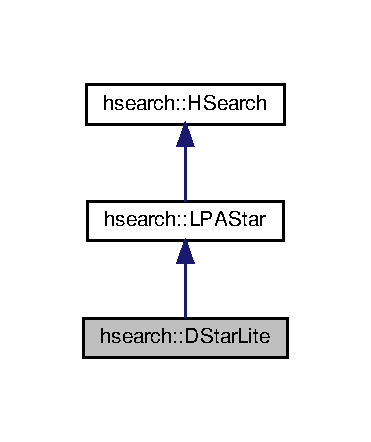
\includegraphics[width=178pt]{d1/d7e/classhsearch_1_1DStarLite__inherit__graph}
\end{center}
\end{figure}


Collaboration diagram for hsearch\+:\+:D\+Star\+Lite\+:\nopagebreak
\begin{figure}[H]
\begin{center}
\leavevmode
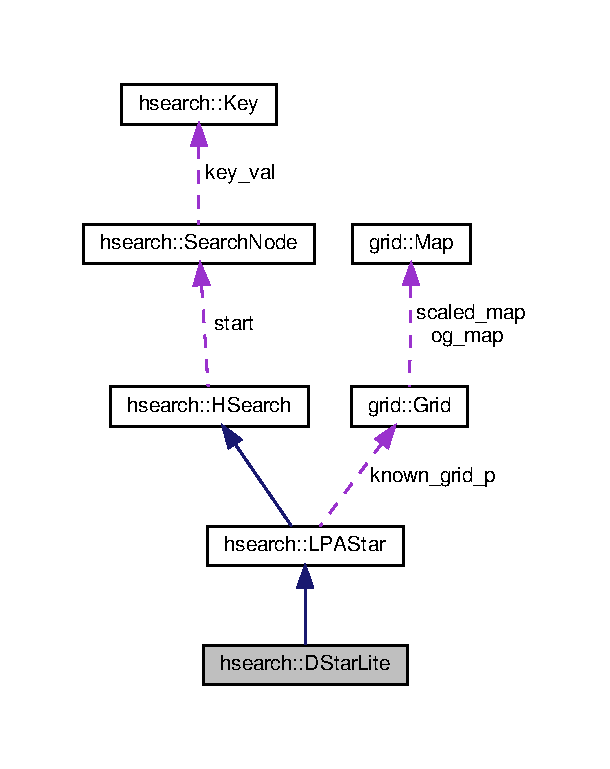
\includegraphics[width=293pt]{d4/d60/classhsearch_1_1DStarLite__coll__graph}
\end{center}
\end{figure}
\subsection*{Public Member Functions}
\begin{DoxyCompactItemize}
\item 
\mbox{\Hypertarget{classhsearch_1_1DStarLite_a0cbed5526d90c0d37261fb501be9cd0a}\label{classhsearch_1_1DStarLite_a0cbed5526d90c0d37261fb501be9cd0a}} 
\hyperlink{classhsearch_1_1DStarLite_a0cbed5526d90c0d37261fb501be9cd0a}{D\+Star\+Lite} ()
\begin{DoxyCompactList}\small\item\em Default Constructor. \end{DoxyCompactList}\item 
\hyperlink{classhsearch_1_1DStarLite_a45691d7cc0afb3ba17e6676bfd96c878}{D\+Star\+Lite} (std\+::vector$<$ std\+::vector$<$ \hyperlink{structprm_1_1Node}{prm\+::\+Node} $>$$>$ $\ast$grid\+\_\+graph, \hyperlink{classgrid_1_1Grid}{grid\+::\+Grid} $\ast$base\+\_\+grid, rigid2d\+::\+Vector2D start\+\_\+loc, rigid2d\+::\+Vector2D \hyperlink{classhsearch_1_1HSearch_a201d281d6a8d9fcc4158772f862d1847}{goal\+\_\+loc})
\begin{DoxyCompactList}\small\item\em provide the search with the beginning state of the map \end{DoxyCompactList}\item 
void \hyperlink{classhsearch_1_1DStarLite_ab4ed525aef3cc48661458cf0e96acfb7}{Update\+Robot\+Loc} (rigid2d\+::\+Vector2D robot\+\_\+loc)
\begin{DoxyCompactList}\small\item\em update the location the search will plan to with the robot\textquotesingle{}s current location, also updates km. Should be called directly before updating the map \end{DoxyCompactList}\end{DoxyCompactItemize}
\subsection*{Additional Inherited Members}


\subsection{Detailed Description}
a class to perform D$\ast$ Lite search 

\subsection{Constructor \& Destructor Documentation}
\mbox{\Hypertarget{classhsearch_1_1DStarLite_a45691d7cc0afb3ba17e6676bfd96c878}\label{classhsearch_1_1DStarLite_a45691d7cc0afb3ba17e6676bfd96c878}} 
\index{hsearch\+::\+D\+Star\+Lite@{hsearch\+::\+D\+Star\+Lite}!D\+Star\+Lite@{D\+Star\+Lite}}
\index{D\+Star\+Lite@{D\+Star\+Lite}!hsearch\+::\+D\+Star\+Lite@{hsearch\+::\+D\+Star\+Lite}}
\subsubsection{\texorpdfstring{D\+Star\+Lite()}{DStarLite()}}
{\footnotesize\ttfamily hsearch\+::\+D\+Star\+Lite\+::\+D\+Star\+Lite (\begin{DoxyParamCaption}\item[{std\+::vector$<$ std\+::vector$<$ \hyperlink{structprm_1_1Node}{prm\+::\+Node} $>$$>$ $\ast$}]{grid\+\_\+graph,  }\item[{\hyperlink{classgrid_1_1Grid}{grid\+::\+Grid} $\ast$}]{base\+\_\+grid,  }\item[{rigid2d\+::\+Vector2D}]{start\+\_\+loc,  }\item[{rigid2d\+::\+Vector2D}]{goal\+\_\+loc }\end{DoxyParamCaption})}



provide the search with the beginning state of the map 


\begin{DoxyParams}{Parameters}
{\em grid\+\_\+graph} & reference to an existing grid \\
\hline
{\em base\+\_\+grid} & pointer to the Grid the search is using \\
\hline
{\em start\+\_\+loc} & the location of the robot in integer coordinates on the provided grid \\
\hline
{\em goal\+\_\+loc} & the location of the goal point in integer coordinates on the provided grid \\
\hline
\end{DoxyParams}


\subsection{Member Function Documentation}
\mbox{\Hypertarget{classhsearch_1_1DStarLite_ab4ed525aef3cc48661458cf0e96acfb7}\label{classhsearch_1_1DStarLite_ab4ed525aef3cc48661458cf0e96acfb7}} 
\index{hsearch\+::\+D\+Star\+Lite@{hsearch\+::\+D\+Star\+Lite}!Update\+Robot\+Loc@{Update\+Robot\+Loc}}
\index{Update\+Robot\+Loc@{Update\+Robot\+Loc}!hsearch\+::\+D\+Star\+Lite@{hsearch\+::\+D\+Star\+Lite}}
\subsubsection{\texorpdfstring{Update\+Robot\+Loc()}{UpdateRobotLoc()}}
{\footnotesize\ttfamily void hsearch\+::\+D\+Star\+Lite\+::\+Update\+Robot\+Loc (\begin{DoxyParamCaption}\item[{rigid2d\+::\+Vector2D}]{robot\+\_\+loc }\end{DoxyParamCaption})}



update the location the search will plan to with the robot\textquotesingle{}s current location, also updates km. Should be called directly before updating the map 


\begin{DoxyParams}{Parameters}
{\em robot\+\_\+loc} & the location of the robot in integer coordinates on the provided grid \\
\hline
\end{DoxyParams}


The documentation for this class was generated from the following files\+:\begin{DoxyCompactItemize}
\item 
global\+\_\+search/include/global\+\_\+search/heuristic\+\_\+search.\+hpp\item 
global\+\_\+search/src/global\+\_\+search/heuristic\+\_\+search.\+cpp\end{DoxyCompactItemize}

\hypertarget{structprm_1_1Edge}{}\section{prm\+:\+:Edge Struct Reference}
\label{structprm_1_1Edge}\index{prm\+::\+Edge@{prm\+::\+Edge}}


A struct to fully describe a connection between two nodes.  




{\ttfamily \#include $<$prm.\+hpp$>$}

\subsection*{Public Attributes}
\begin{DoxyCompactItemize}
\item 
\mbox{\Hypertarget{structprm_1_1Edge_ac0e99ee22ee177b40873843765182041}\label{structprm_1_1Edge_ac0e99ee22ee177b40873843765182041}} 
int \hyperlink{structprm_1_1Edge_ac0e99ee22ee177b40873843765182041}{edge\+\_\+id} = -\/1
\begin{DoxyCompactList}\small\item\em A unique ID for the edge. \end{DoxyCompactList}\item 
\mbox{\Hypertarget{structprm_1_1Edge_a9a0ca060886a2e8be43e0c84683d0084}\label{structprm_1_1Edge_a9a0ca060886a2e8be43e0c84683d0084}} 
int \hyperlink{structprm_1_1Edge_a9a0ca060886a2e8be43e0c84683d0084}{node1\+\_\+id} = -\/1
\begin{DoxyCompactList}\small\item\em The parent node ID. \end{DoxyCompactList}\item 
\mbox{\Hypertarget{structprm_1_1Edge_a40d4adffbf6bb4d9ec63531b51ca845e}\label{structprm_1_1Edge_a40d4adffbf6bb4d9ec63531b51ca845e}} 
rigid2d\+::\+Vector2D \hyperlink{structprm_1_1Edge_a40d4adffbf6bb4d9ec63531b51ca845e}{node1}
\begin{DoxyCompactList}\small\item\em the parent node location \end{DoxyCompactList}\item 
\mbox{\Hypertarget{structprm_1_1Edge_a46beeb0a5adb2a6777db2a6a0986fff4}\label{structprm_1_1Edge_a46beeb0a5adb2a6777db2a6a0986fff4}} 
int \hyperlink{structprm_1_1Edge_a46beeb0a5adb2a6777db2a6a0986fff4}{node2\+\_\+id} = -\/1
\begin{DoxyCompactList}\small\item\em the child node ID \end{DoxyCompactList}\item 
\mbox{\Hypertarget{structprm_1_1Edge_a3d555282fbb49f6cbaa37865ae09029c}\label{structprm_1_1Edge_a3d555282fbb49f6cbaa37865ae09029c}} 
rigid2d\+::\+Vector2D \hyperlink{structprm_1_1Edge_a3d555282fbb49f6cbaa37865ae09029c}{node2}
\begin{DoxyCompactList}\small\item\em the child node location \end{DoxyCompactList}\item 
\mbox{\Hypertarget{structprm_1_1Edge_a7f65f07649f06a87bc16514c75b9feb2}\label{structprm_1_1Edge_a7f65f07649f06a87bc16514c75b9feb2}} 
double \hyperlink{structprm_1_1Edge_a7f65f07649f06a87bc16514c75b9feb2}{distance}
\begin{DoxyCompactList}\small\item\em length of the edge \end{DoxyCompactList}\end{DoxyCompactItemize}


\subsection{Detailed Description}
A struct to fully describe a connection between two nodes. 

The documentation for this struct was generated from the following file\+:\begin{DoxyCompactItemize}
\item 
roadmap/include/roadmap/prm.\+hpp\end{DoxyCompactItemize}

\hypertarget{classgrid_1_1Grid}{}\section{grid\+:\+:Grid Class Reference}
\label{classgrid_1_1Grid}\index{grid\+::\+Grid@{grid\+::\+Grid}}


Class to create a \hyperlink{classgrid_1_1Grid}{Grid} overlay for provided \hyperlink{structgrid_1_1Map}{Map} information.  




{\ttfamily \#include $<$grid.\+hpp$>$}



Collaboration diagram for grid\+:\+:Grid\+:\nopagebreak
\begin{figure}[H]
\begin{center}
\leavevmode
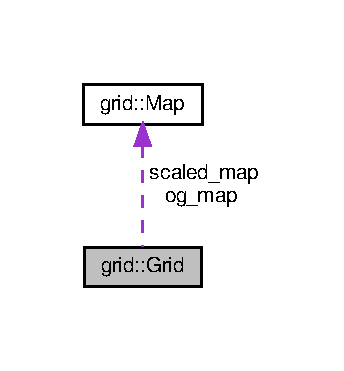
\includegraphics[width=165pt]{dc/d43/classgrid_1_1Grid__coll__graph}
\end{center}
\end{figure}
\subsection*{Public Member Functions}
\begin{DoxyCompactItemize}
\item 
\mbox{\Hypertarget{classgrid_1_1Grid_afcee115a9437842956e1efe9e202c302}\label{classgrid_1_1Grid_afcee115a9437842956e1efe9e202c302}} 
\hyperlink{classgrid_1_1Grid_afcee115a9437842956e1efe9e202c302}{Grid} ()
\begin{DoxyCompactList}\small\item\em Initialization to construct a grid in an empty 10x10 area. \end{DoxyCompactList}\item 
\hyperlink{classgrid_1_1Grid_a39cd30c1ee231fde7f5a3f228a326ac1}{Grid} (std\+::vector$<$ double $>$ xboundary, std\+::vector$<$ double $>$ yboundary)
\begin{DoxyCompactList}\small\item\em Initialization to construct a grid in an empty user defined area. \end{DoxyCompactList}\item 
\hyperlink{classgrid_1_1Grid_a3fd6c9bb56bc7ae63d6126312e001f23}{Grid} (std\+::vector$<$ std\+::vector$<$ rigid2d\+::\+Vector2D $>$$>$ polygon\+\_\+verticies, std\+::vector$<$ double $>$ xboundary, std\+::vector$<$ double $>$ yboundary)
\begin{DoxyCompactList}\small\item\em Initialization to construct a grid in a user defined area with obstacles. \end{DoxyCompactList}\item 
void \hyperlink{classgrid_1_1Grid_adcba03289a5d2de6e209b2a3ded5d5ac}{build\+\_\+grid} (double \hyperlink{classgrid_1_1Grid_acb1ca003a2aeafe6b554d9ac27b29109}{cell\+\_\+size}, unsigned int \hyperlink{classgrid_1_1Grid_a574ec32cb3346c1be8de79ccc38cd47b}{grid\+\_\+res}, double robot\+\_\+radius)
\begin{DoxyCompactList}\small\item\em Function to call all nessissary functions to build the grid. \end{DoxyCompactList}\item 
\mbox{\Hypertarget{classgrid_1_1Grid_a6620e51207bbd6ca60f868b120cb7e04}\label{classgrid_1_1Grid_a6620e51207bbd6ca60f868b120cb7e04}} 
void \hyperlink{classgrid_1_1Grid_a6620e51207bbd6ca60f868b120cb7e04}{generate\+\_\+centers\+\_\+graph} ()
\begin{DoxyCompactList}\small\item\em Function to generate an 8 neighbor connected graph structure based on grid cell center locations. \end{DoxyCompactList}\item 
std\+::vector$<$ int $>$ \hyperlink{classgrid_1_1Grid_adc9dda8d5d6bca20697790712b154cc1}{update\+\_\+grid} (std\+::vector$<$ std\+::pair$<$ rigid2d\+::\+Vector2D, signed char $>$$>$ points)
\begin{DoxyCompactList}\small\item\em Update the existing occupancy data with new information -\/ Note this does not update the stored \hyperlink{structgrid_1_1Map}{Map} variables, so calling \char`\"{}build\+\_\+grid\char`\"{} will revert the occ data based on the map used to create the grid. \end{DoxyCompactList}\item 
std\+::vector$<$ std\+::vector$<$ \hyperlink{structprm_1_1Node}{prm\+::\+Node} $>$ $>$ \hyperlink{classgrid_1_1Grid_a28e01687d0e3e922607e67b3d1d862b6}{get\+\_\+nodes} () const
\begin{DoxyCompactList}\small\item\em Retrive the nodes in a 2D vector in the shape of the grid. \end{DoxyCompactList}\item 
std\+::vector$<$ \hyperlink{structprm_1_1Node}{prm\+::\+Node} $>$ \hyperlink{classgrid_1_1Grid_adc6f8296117527ab16f352806e9dc1d6}{get\+\_\+nodes\+\_\+flatten} () const
\begin{DoxyCompactList}\small\item\em Retrive the nodes in row major order. \end{DoxyCompactList}\item 
std\+::vector$<$ \hyperlink{structprm_1_1Edge}{prm\+::\+Edge} $>$ \hyperlink{classgrid_1_1Grid_a22f08e25cb643d8813fc4332300185b7}{get\+\_\+edges} () const
\begin{DoxyCompactList}\small\item\em Retrive the unique edges in the graph. \end{DoxyCompactList}\item 
std\+::vector$<$ std\+::vector$<$ signed char $>$ $>$ \hyperlink{classgrid_1_1Grid_a9efaa72e19c8351e1979c6ac18517de4}{get\+\_\+grid} () const
\begin{DoxyCompactList}\small\item\em retrieve the built grid \end{DoxyCompactList}\item 
std\+::vector$<$ signed char $>$ \hyperlink{classgrid_1_1Grid_a7c05ad9408e0ff99e36a3196136f3bb7}{get\+\_\+grid\+\_\+flatten} () const
\begin{DoxyCompactList}\small\item\em convert the grid data into a in row major order with the first element corresponding to the lower left corner. \end{DoxyCompactList}\item 
std\+::vector$<$ int $>$ \hyperlink{classgrid_1_1Grid_ab5da2712457e615bb12ca6d5fc1f1b9d}{get\+\_\+grid\+\_\+dimensions} () const
\begin{DoxyCompactList}\small\item\em get the height and width of the grid \end{DoxyCompactList}\item 
rigid2d\+::\+Vector2D \hyperlink{classgrid_1_1Grid_a740d72189efbdf5595c3ddaacc8cdfc4}{grid\+\_\+to\+\_\+world} (rigid2d\+::\+Vector2D grid\+\_\+coord)
\begin{DoxyCompactList}\small\item\em convert from grid coordinates (integers) to world coordinates (meters) \end{DoxyCompactList}\item 
rigid2d\+::\+Vector2D \hyperlink{classgrid_1_1Grid_a9aeb33485b294ab4a07178359db6e3cf}{world\+\_\+to\+\_\+grid} (rigid2d\+::\+Vector2D world\+\_\+coord)
\begin{DoxyCompactList}\small\item\em convert from world coordinates to grid coordinates \end{DoxyCompactList}\end{DoxyCompactItemize}
\subsection*{Private Member Functions}
\begin{DoxyCompactItemize}
\item 
\mbox{\Hypertarget{classgrid_1_1Grid_af5dd6a34ea30b975c4e72304db4e6dc7}\label{classgrid_1_1Grid_af5dd6a34ea30b975c4e72304db4e6dc7}} 
void \hyperlink{classgrid_1_1Grid_af5dd6a34ea30b975c4e72304db4e6dc7}{grid\+\_\+resize} ()
\begin{DoxyCompactList}\small\item\em calculate the grid size based on the saved map and the grid resolution \end{DoxyCompactList}\item 
bool \hyperlink{classgrid_1_1Grid_a5b8625b7400116c5707c0465467a597d}{cell\+\_\+near\+\_\+boarder} (rigid2d\+::\+Vector2D center, double threshold)
\begin{DoxyCompactList}\small\item\em Determine if the cell center is within the buffer radius of the map boarder. \end{DoxyCompactList}\end{DoxyCompactItemize}
\subsection*{Private Attributes}
\begin{DoxyCompactItemize}
\item 
\mbox{\Hypertarget{classgrid_1_1Grid_a611cf14f1d75f0c77a7a5bcbc8fee6e0}\label{classgrid_1_1Grid_a611cf14f1d75f0c77a7a5bcbc8fee6e0}} 
\hyperlink{structgrid_1_1Map}{Map} \hyperlink{classgrid_1_1Grid_a611cf14f1d75f0c77a7a5bcbc8fee6e0}{og\+\_\+map}
\begin{DoxyCompactList}\small\item\em the map to initialize the grid with \end{DoxyCompactList}\item 
\mbox{\Hypertarget{classgrid_1_1Grid_ab990be4a53fd45a83df3f823f7098d56}\label{classgrid_1_1Grid_ab990be4a53fd45a83df3f823f7098d56}} 
\hyperlink{structgrid_1_1Map}{Map} \hyperlink{classgrid_1_1Grid_ab990be4a53fd45a83df3f823f7098d56}{scaled\+\_\+map}
\begin{DoxyCompactList}\small\item\em the scaled map based on the grid resolution \end{DoxyCompactList}\item 
\mbox{\Hypertarget{classgrid_1_1Grid_a375f27f536721667f4487b74982c154a}\label{classgrid_1_1Grid_a375f27f536721667f4487b74982c154a}} 
std\+::vector$<$ int $>$ \hyperlink{classgrid_1_1Grid_a375f27f536721667f4487b74982c154a}{grid\+\_\+dimensions}
\begin{DoxyCompactList}\small\item\em x, y \end{DoxyCompactList}\item 
\mbox{\Hypertarget{classgrid_1_1Grid_aae353051de1a48dd8f29e1889d71bf88}\label{classgrid_1_1Grid_aae353051de1a48dd8f29e1889d71bf88}} 
double \hyperlink{classgrid_1_1Grid_aae353051de1a48dd8f29e1889d71bf88}{buffer\+\_\+radius} = 0.\+0
\begin{DoxyCompactList}\small\item\em buffer distance to incorporate when detecting collisions \end{DoxyCompactList}\item 
\mbox{\Hypertarget{classgrid_1_1Grid_a574ec32cb3346c1be8de79ccc38cd47b}\label{classgrid_1_1Grid_a574ec32cb3346c1be8de79ccc38cd47b}} 
unsigned int \hyperlink{classgrid_1_1Grid_a574ec32cb3346c1be8de79ccc38cd47b}{grid\+\_\+res} = 1
\begin{DoxyCompactList}\small\item\em scale the cell size \end{DoxyCompactList}\item 
\mbox{\Hypertarget{classgrid_1_1Grid_acb1ca003a2aeafe6b554d9ac27b29109}\label{classgrid_1_1Grid_acb1ca003a2aeafe6b554d9ac27b29109}} 
double \hyperlink{classgrid_1_1Grid_acb1ca003a2aeafe6b554d9ac27b29109}{cell\+\_\+size} = 1.\+0
\begin{DoxyCompactList}\small\item\em meters per grid cell \end{DoxyCompactList}\item 
\mbox{\Hypertarget{classgrid_1_1Grid_a970c0980c3a662ddaddd9e457f799252}\label{classgrid_1_1Grid_a970c0980c3a662ddaddd9e457f799252}} 
std\+::vector$<$ std\+::vector$<$ \hyperlink{structprm_1_1Node}{prm\+::\+Node} $>$ $>$ \hyperlink{classgrid_1_1Grid_a970c0980c3a662ddaddd9e457f799252}{nodes}
\begin{DoxyCompactList}\small\item\em all nodes in the grid \end{DoxyCompactList}\item 
\mbox{\Hypertarget{classgrid_1_1Grid_a80fab4482c55128e29083184c234f197}\label{classgrid_1_1Grid_a80fab4482c55128e29083184c234f197}} 
std\+::vector$<$ \hyperlink{structprm_1_1Edge}{prm\+::\+Edge} $>$ \hyperlink{classgrid_1_1Grid_a80fab4482c55128e29083184c234f197}{all\+\_\+edges}
\begin{DoxyCompactList}\small\item\em all edges between the grid \end{DoxyCompactList}\item 
\mbox{\Hypertarget{classgrid_1_1Grid_a640e9d8f352ebb19ec2801229e5483e4}\label{classgrid_1_1Grid_a640e9d8f352ebb19ec2801229e5483e4}} 
std\+::vector$<$ std\+::vector$<$ signed char $>$ $>$ \hyperlink{classgrid_1_1Grid_a640e9d8f352ebb19ec2801229e5483e4}{occ\+\_\+data}
\begin{DoxyCompactList}\small\item\em occupancy grid data, 0 is free, 50 is buffer zone, 100 is occupied \end{DoxyCompactList}\end{DoxyCompactItemize}


\subsection{Detailed Description}
Class to create a \hyperlink{classgrid_1_1Grid}{Grid} overlay for provided \hyperlink{structgrid_1_1Map}{Map} information. 

\subsection{Constructor \& Destructor Documentation}
\mbox{\Hypertarget{classgrid_1_1Grid_a39cd30c1ee231fde7f5a3f228a326ac1}\label{classgrid_1_1Grid_a39cd30c1ee231fde7f5a3f228a326ac1}} 
\index{grid\+::\+Grid@{grid\+::\+Grid}!Grid@{Grid}}
\index{Grid@{Grid}!grid\+::\+Grid@{grid\+::\+Grid}}
\subsubsection{\texorpdfstring{Grid()}{Grid()}\hspace{0.1cm}{\footnotesize\ttfamily [1/2]}}
{\footnotesize\ttfamily grid\+::\+Grid\+::\+Grid (\begin{DoxyParamCaption}\item[{std\+::vector$<$ double $>$}]{xboundary,  }\item[{std\+::vector$<$ double $>$}]{yboundary }\end{DoxyParamCaption})}



Initialization to construct a grid in an empty user defined area. 


\begin{DoxyParams}{Parameters}
{\em xboundary} & a 2 element vector defining the map\textquotesingle{}s x bounds in integer coordinates \\
\hline
{\em yboundary} & a 2 element vector defining the map\textquotesingle{}s y bounds in integer coordinates \\
\hline
\end{DoxyParams}
\mbox{\Hypertarget{classgrid_1_1Grid_a3fd6c9bb56bc7ae63d6126312e001f23}\label{classgrid_1_1Grid_a3fd6c9bb56bc7ae63d6126312e001f23}} 
\index{grid\+::\+Grid@{grid\+::\+Grid}!Grid@{Grid}}
\index{Grid@{Grid}!grid\+::\+Grid@{grid\+::\+Grid}}
\subsubsection{\texorpdfstring{Grid()}{Grid()}\hspace{0.1cm}{\footnotesize\ttfamily [2/2]}}
{\footnotesize\ttfamily grid\+::\+Grid\+::\+Grid (\begin{DoxyParamCaption}\item[{std\+::vector$<$ std\+::vector$<$ rigid2d\+::\+Vector2D $>$$>$}]{polygon\+\_\+verticies,  }\item[{std\+::vector$<$ double $>$}]{xboundary,  }\item[{std\+::vector$<$ double $>$}]{yboundary }\end{DoxyParamCaption})}



Initialization to construct a grid in a user defined area with obstacles. 


\begin{DoxyParams}{Parameters}
{\em polygon\+\_\+verticies} & a vector of vectors defining the verticies of each obstacle in integer coordinates and in order going counter-\/clockwise \\
\hline
{\em xboundary} & a 2 element vector defining the map\textquotesingle{}s x bounds in integer coordinates \\
\hline
{\em yboundary} & a 2 element vector defining the map\textquotesingle{}s y bounds in integer coordinates \\
\hline
\end{DoxyParams}


\subsection{Member Function Documentation}
\mbox{\Hypertarget{classgrid_1_1Grid_adcba03289a5d2de6e209b2a3ded5d5ac}\label{classgrid_1_1Grid_adcba03289a5d2de6e209b2a3ded5d5ac}} 
\index{grid\+::\+Grid@{grid\+::\+Grid}!build\+\_\+grid@{build\+\_\+grid}}
\index{build\+\_\+grid@{build\+\_\+grid}!grid\+::\+Grid@{grid\+::\+Grid}}
\subsubsection{\texorpdfstring{build\+\_\+grid()}{build\_grid()}}
{\footnotesize\ttfamily void grid\+::\+Grid\+::build\+\_\+grid (\begin{DoxyParamCaption}\item[{double}]{cell\+\_\+size,  }\item[{unsigned int}]{grid\+\_\+res,  }\item[{double}]{robot\+\_\+radius }\end{DoxyParamCaption})}



Function to call all nessissary functions to build the grid. 


\begin{DoxyParams}{Parameters}
{\em cell\+\_\+size} & the desired distance the distance for the cell length/height in meters \\
\hline
{\em grid\+\_\+res} & scaling factor to create the occupancy grid with a finer resolution that the existing cell\+\_\+size. Use 1 to make the grid equal to the current cell size Use 2 to double the resolution. \\
\hline
{\em robot\+\_\+radius} & the radius to use as a buffer around the robot for collision detection \\
\hline
\end{DoxyParams}
\mbox{\Hypertarget{classgrid_1_1Grid_a5b8625b7400116c5707c0465467a597d}\label{classgrid_1_1Grid_a5b8625b7400116c5707c0465467a597d}} 
\index{grid\+::\+Grid@{grid\+::\+Grid}!cell\+\_\+near\+\_\+boarder@{cell\+\_\+near\+\_\+boarder}}
\index{cell\+\_\+near\+\_\+boarder@{cell\+\_\+near\+\_\+boarder}!grid\+::\+Grid@{grid\+::\+Grid}}
\subsubsection{\texorpdfstring{cell\+\_\+near\+\_\+boarder()}{cell\_near\_boarder()}}
{\footnotesize\ttfamily bool grid\+::\+Grid\+::cell\+\_\+near\+\_\+boarder (\begin{DoxyParamCaption}\item[{rigid2d\+::\+Vector2D}]{center,  }\item[{double}]{threshold }\end{DoxyParamCaption})\hspace{0.3cm}{\ttfamily [private]}}



Determine if the cell center is within the buffer radius of the map boarder. 


\begin{DoxyParams}{Parameters}
{\em center} & location of cell to check against \\
\hline
{\em threshold} & grid buffer distance \\
\hline
\end{DoxyParams}
\begin{DoxyReturn}{Returns}
True if the cell center is within the buffer\+\_\+radius 
\end{DoxyReturn}
\mbox{\Hypertarget{classgrid_1_1Grid_a22f08e25cb643d8813fc4332300185b7}\label{classgrid_1_1Grid_a22f08e25cb643d8813fc4332300185b7}} 
\index{grid\+::\+Grid@{grid\+::\+Grid}!get\+\_\+edges@{get\+\_\+edges}}
\index{get\+\_\+edges@{get\+\_\+edges}!grid\+::\+Grid@{grid\+::\+Grid}}
\subsubsection{\texorpdfstring{get\+\_\+edges()}{get\_edges()}}
{\footnotesize\ttfamily std\+::vector$<$ \hyperlink{structprm_1_1Edge}{prm\+::\+Edge} $>$ grid\+::\+Grid\+::get\+\_\+edges (\begin{DoxyParamCaption}{ }\end{DoxyParamCaption}) const}



Retrive the unique edges in the graph. 

\begin{DoxyReturn}{Returns}
all the unique edges 
\end{DoxyReturn}
\mbox{\Hypertarget{classgrid_1_1Grid_a9efaa72e19c8351e1979c6ac18517de4}\label{classgrid_1_1Grid_a9efaa72e19c8351e1979c6ac18517de4}} 
\index{grid\+::\+Grid@{grid\+::\+Grid}!get\+\_\+grid@{get\+\_\+grid}}
\index{get\+\_\+grid@{get\+\_\+grid}!grid\+::\+Grid@{grid\+::\+Grid}}
\subsubsection{\texorpdfstring{get\+\_\+grid()}{get\_grid()}}
{\footnotesize\ttfamily std\+::vector$<$ std\+::vector$<$ signed char $>$ $>$ grid\+::\+Grid\+::get\+\_\+grid (\begin{DoxyParamCaption}{ }\end{DoxyParamCaption}) const}



retrieve the built grid 

\begin{DoxyReturn}{Returns}
grid occupancy data as a vector of vectors. 
\end{DoxyReturn}
\mbox{\Hypertarget{classgrid_1_1Grid_ab5da2712457e615bb12ca6d5fc1f1b9d}\label{classgrid_1_1Grid_ab5da2712457e615bb12ca6d5fc1f1b9d}} 
\index{grid\+::\+Grid@{grid\+::\+Grid}!get\+\_\+grid\+\_\+dimensions@{get\+\_\+grid\+\_\+dimensions}}
\index{get\+\_\+grid\+\_\+dimensions@{get\+\_\+grid\+\_\+dimensions}!grid\+::\+Grid@{grid\+::\+Grid}}
\subsubsection{\texorpdfstring{get\+\_\+grid\+\_\+dimensions()}{get\_grid\_dimensions()}}
{\footnotesize\ttfamily std\+::vector$<$ int $>$ grid\+::\+Grid\+::get\+\_\+grid\+\_\+dimensions (\begin{DoxyParamCaption}{ }\end{DoxyParamCaption}) const}



get the height and width of the grid 

\begin{DoxyReturn}{Returns}
the grid dimensions in number of cells 
\end{DoxyReturn}
\mbox{\Hypertarget{classgrid_1_1Grid_a7c05ad9408e0ff99e36a3196136f3bb7}\label{classgrid_1_1Grid_a7c05ad9408e0ff99e36a3196136f3bb7}} 
\index{grid\+::\+Grid@{grid\+::\+Grid}!get\+\_\+grid\+\_\+flatten@{get\+\_\+grid\+\_\+flatten}}
\index{get\+\_\+grid\+\_\+flatten@{get\+\_\+grid\+\_\+flatten}!grid\+::\+Grid@{grid\+::\+Grid}}
\subsubsection{\texorpdfstring{get\+\_\+grid\+\_\+flatten()}{get\_grid\_flatten()}}
{\footnotesize\ttfamily std\+::vector$<$ signed char $>$ grid\+::\+Grid\+::get\+\_\+grid\+\_\+flatten (\begin{DoxyParamCaption}{ }\end{DoxyParamCaption}) const}



convert the grid data into a in row major order with the first element corresponding to the lower left corner. 

\begin{DoxyReturn}{Returns}
grid occupancy data in row major order 
\end{DoxyReturn}
\mbox{\Hypertarget{classgrid_1_1Grid_a28e01687d0e3e922607e67b3d1d862b6}\label{classgrid_1_1Grid_a28e01687d0e3e922607e67b3d1d862b6}} 
\index{grid\+::\+Grid@{grid\+::\+Grid}!get\+\_\+nodes@{get\+\_\+nodes}}
\index{get\+\_\+nodes@{get\+\_\+nodes}!grid\+::\+Grid@{grid\+::\+Grid}}
\subsubsection{\texorpdfstring{get\+\_\+nodes()}{get\_nodes()}}
{\footnotesize\ttfamily std\+::vector$<$ std\+::vector$<$ \hyperlink{structprm_1_1Node}{prm\+::\+Node} $>$ $>$ grid\+::\+Grid\+::get\+\_\+nodes (\begin{DoxyParamCaption}{ }\end{DoxyParamCaption}) const}



Retrive the nodes in a 2D vector in the shape of the grid. 

\begin{DoxyReturn}{Returns}
the nodes in a structure matching the grid 
\end{DoxyReturn}
\mbox{\Hypertarget{classgrid_1_1Grid_adc6f8296117527ab16f352806e9dc1d6}\label{classgrid_1_1Grid_adc6f8296117527ab16f352806e9dc1d6}} 
\index{grid\+::\+Grid@{grid\+::\+Grid}!get\+\_\+nodes\+\_\+flatten@{get\+\_\+nodes\+\_\+flatten}}
\index{get\+\_\+nodes\+\_\+flatten@{get\+\_\+nodes\+\_\+flatten}!grid\+::\+Grid@{grid\+::\+Grid}}
\subsubsection{\texorpdfstring{get\+\_\+nodes\+\_\+flatten()}{get\_nodes\_flatten()}}
{\footnotesize\ttfamily std\+::vector$<$ \hyperlink{structprm_1_1Node}{prm\+::\+Node} $>$ grid\+::\+Grid\+::get\+\_\+nodes\+\_\+flatten (\begin{DoxyParamCaption}{ }\end{DoxyParamCaption}) const}



Retrive the nodes in row major order. 

\begin{DoxyReturn}{Returns}
the nodes in a single row vector 
\end{DoxyReturn}
\mbox{\Hypertarget{classgrid_1_1Grid_a740d72189efbdf5595c3ddaacc8cdfc4}\label{classgrid_1_1Grid_a740d72189efbdf5595c3ddaacc8cdfc4}} 
\index{grid\+::\+Grid@{grid\+::\+Grid}!grid\+\_\+to\+\_\+world@{grid\+\_\+to\+\_\+world}}
\index{grid\+\_\+to\+\_\+world@{grid\+\_\+to\+\_\+world}!grid\+::\+Grid@{grid\+::\+Grid}}
\subsubsection{\texorpdfstring{grid\+\_\+to\+\_\+world()}{grid\_to\_world()}}
{\footnotesize\ttfamily rigid2d\+::\+Vector2D grid\+::\+Grid\+::grid\+\_\+to\+\_\+world (\begin{DoxyParamCaption}\item[{rigid2d\+::\+Vector2D}]{grid\+\_\+coord }\end{DoxyParamCaption})}



convert from grid coordinates (integers) to world coordinates (meters) 


\begin{DoxyParams}{Parameters}
{\em grid\+\_\+coord} & grid location to convert \\
\hline
\end{DoxyParams}
\begin{DoxyReturn}{Returns}
matching world coordinate 
\end{DoxyReturn}
\mbox{\Hypertarget{classgrid_1_1Grid_adc9dda8d5d6bca20697790712b154cc1}\label{classgrid_1_1Grid_adc9dda8d5d6bca20697790712b154cc1}} 
\index{grid\+::\+Grid@{grid\+::\+Grid}!update\+\_\+grid@{update\+\_\+grid}}
\index{update\+\_\+grid@{update\+\_\+grid}!grid\+::\+Grid@{grid\+::\+Grid}}
\subsubsection{\texorpdfstring{update\+\_\+grid()}{update\_grid()}}
{\footnotesize\ttfamily std\+::vector$<$ int $>$ grid\+::\+Grid\+::update\+\_\+grid (\begin{DoxyParamCaption}\item[{std\+::vector$<$ std\+::pair$<$ rigid2d\+::\+Vector2D, signed char $>$$>$}]{points }\end{DoxyParamCaption})}



Update the existing occupancy data with new information -\/ Note this does not update the stored \hyperlink{structgrid_1_1Map}{Map} variables, so calling \char`\"{}build\+\_\+grid\char`\"{} will revert the occ data based on the map used to create the grid. 


\begin{DoxyParams}{Parameters}
{\em points} & pairs of grid cell locations and new occupancy data to potentially update. \\
\hline
\end{DoxyParams}
\begin{DoxyReturn}{Returns}
a vector of boolean values\+: True if the new point info actually caused a change in the occupancy data from free to occupied, otherwise False. 
\end{DoxyReturn}
\mbox{\Hypertarget{classgrid_1_1Grid_a9aeb33485b294ab4a07178359db6e3cf}\label{classgrid_1_1Grid_a9aeb33485b294ab4a07178359db6e3cf}} 
\index{grid\+::\+Grid@{grid\+::\+Grid}!world\+\_\+to\+\_\+grid@{world\+\_\+to\+\_\+grid}}
\index{world\+\_\+to\+\_\+grid@{world\+\_\+to\+\_\+grid}!grid\+::\+Grid@{grid\+::\+Grid}}
\subsubsection{\texorpdfstring{world\+\_\+to\+\_\+grid()}{world\_to\_grid()}}
{\footnotesize\ttfamily rigid2d\+::\+Vector2D grid\+::\+Grid\+::world\+\_\+to\+\_\+grid (\begin{DoxyParamCaption}\item[{rigid2d\+::\+Vector2D}]{world\+\_\+coord }\end{DoxyParamCaption})}



convert from world coordinates to grid coordinates 


\begin{DoxyParams}{Parameters}
{\em world\+\_\+coord} & world location to convert \\
\hline
\end{DoxyParams}
\begin{DoxyReturn}{Returns}
matching grid coordinate 
\end{DoxyReturn}


The documentation for this class was generated from the following files\+:\begin{DoxyCompactItemize}
\item 
roadmap/include/roadmap/grid.\+hpp\item 
roadmap/src/roadmap/grid.\+cpp\end{DoxyCompactItemize}

\hypertarget{classhsearch_1_1HSearch}{}\section{hsearch\+:\+:H\+Search Class Reference}
\label{classhsearch_1_1HSearch}\index{hsearch\+::\+H\+Search@{hsearch\+::\+H\+Search}}


The base class to define a heuristic based search algorithm. This class has no Compute\+Cost funtion which is required to find the shortest path. This function is defined in the derived class to determine the type of search. Some searched also have a different flow for finding the shortest path, which is why the Compute\+Shortest\+Path method is virtual. Currently this class will only plan against a precontructed graph.  




{\ttfamily \#include $<$heuristic\+\_\+search.\+hpp$>$}



Inheritance diagram for hsearch\+:\+:H\+Search\+:\nopagebreak
\begin{figure}[H]
\begin{center}
\leavevmode
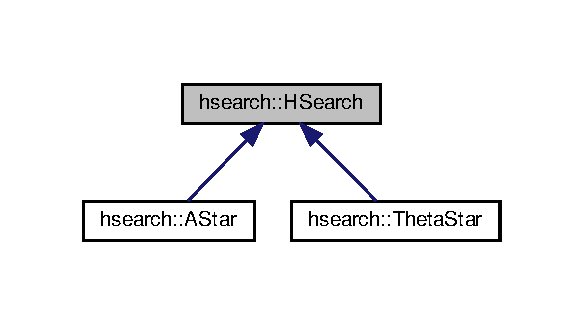
\includegraphics[width=350pt]{d3/dff/classhsearch_1_1HSearch__inherit__graph}
\end{center}
\end{figure}


Collaboration diagram for hsearch\+:\+:H\+Search\+:\nopagebreak
\begin{figure}[H]
\begin{center}
\leavevmode
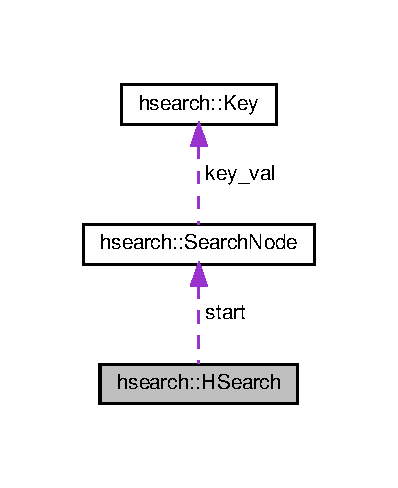
\includegraphics[width=191pt]{df/d1e/classhsearch_1_1HSearch__coll__graph}
\end{center}
\end{figure}
\subsection*{Public Member Functions}
\begin{DoxyCompactItemize}
\item 
\mbox{\Hypertarget{classhsearch_1_1HSearch_a88c750ab9e6c9ad303f468ef270619c3}\label{classhsearch_1_1HSearch_a88c750ab9e6c9ad303f468ef270619c3}} 
\hyperlink{classhsearch_1_1HSearch_a88c750ab9e6c9ad303f468ef270619c3}{H\+Search} ()
\begin{DoxyCompactList}\small\item\em default constructor \end{DoxyCompactList}\item 
\hyperlink{classhsearch_1_1HSearch_a52aed9d8d8c634bd506cfd3c14620884}{H\+Search} (std\+::vector$<$ \hyperlink{structprm_1_1Node}{prm\+::\+Node} $>$ $\ast$node\+\_\+list)
\begin{DoxyCompactList}\small\item\em Initialize the search with a precontructed graph. \end{DoxyCompactList}\item 
\hyperlink{classhsearch_1_1HSearch_a58bce8362211fa679ebf8200dc31d03d}{H\+Search} (\hyperlink{structgrid_1_1Map}{grid\+::\+Map} map)
\begin{DoxyCompactList}\small\item\em Initialize the search with a precontructed graph. \end{DoxyCompactList}\item 
\mbox{\Hypertarget{classhsearch_1_1HSearch_ab48be1a6bdbd923ce5e83f6b39323941}\label{classhsearch_1_1HSearch_ab48be1a6bdbd923ce5e83f6b39323941}} 
virtual \hyperlink{classhsearch_1_1HSearch_ab48be1a6bdbd923ce5e83f6b39323941}{$\sim$\+H\+Search} ()=default
\begin{DoxyCompactList}\small\item\em Use default destructor for this and all derived classes. \end{DoxyCompactList}\item 
virtual bool \hyperlink{classhsearch_1_1HSearch_a8641b99479bbdf017bf5a1168b763c27}{Compute\+Shortest\+Path} (const \hyperlink{structprm_1_1Node}{prm\+::\+Node} \&s\+\_\+start, const \hyperlink{structprm_1_1Node}{prm\+::\+Node} \&s\+\_\+goal)
\begin{DoxyCompactList}\small\item\em The main routine for the search algorithm. \end{DoxyCompactList}\item 
std\+::vector$<$ rigid2d\+::\+Vector2D $>$ \hyperlink{classhsearch_1_1HSearch_a2dbcfc312e89d60d9ec9b85eef271cbf}{get\+\_\+path} ()
\begin{DoxyCompactList}\small\item\em All the user to retrive the final path. \end{DoxyCompactList}\item 
std\+::vector$<$ rigid2d\+::\+Vector2D $>$ \hyperlink{classhsearch_1_1HSearch_a93b63eb8983863eb40f7bb1f28af5c36}{get\+\_\+expanded\+\_\+nodes} ()
\begin{DoxyCompactList}\small\item\em Get all of the nodes expanded during the search. \end{DoxyCompactList}\end{DoxyCompactItemize}
\subsection*{Protected Member Functions}
\begin{DoxyCompactItemize}
\item 
virtual void \hyperlink{classhsearch_1_1HSearch_a5d325955c4faedaca0c68155fd1f7e69}{Compute\+Cost} (\hyperlink{structhsearch_1_1SearchNode}{Search\+Node} \&s, \hyperlink{structhsearch_1_1SearchNode}{Search\+Node} \&sp)=0
\begin{DoxyCompactList}\small\item\em a function used to compute the cost for a pair of nodes \end{DoxyCompactList}\item 
virtual void \hyperlink{classhsearch_1_1HSearch_ac94c08c0f0d4cc3076f01d70c6cd7679}{assemble\+\_\+path} (\hyperlink{structhsearch_1_1SearchNode}{Search\+Node} goal)
\begin{DoxyCompactList}\small\item\em build the final path based on all of the saved pointers \end{DoxyCompactList}\item 
std\+::vector$<$ double $>$ \hyperlink{classhsearch_1_1HSearch_a6ca884af67da489fa1b20592abc1dbba}{f} (\hyperlink{structhsearch_1_1SearchNode}{Search\+Node} s, \hyperlink{structhsearch_1_1SearchNode}{Search\+Node} sp)
\begin{DoxyCompactList}\small\item\em calculate the total cost of a node \end{DoxyCompactList}\item 
double \hyperlink{classhsearch_1_1HSearch_a687960c8dcfc61e16613a72a4ff1c14d}{g} (\hyperlink{structhsearch_1_1SearchNode}{Search\+Node} s, \hyperlink{structhsearch_1_1SearchNode}{Search\+Node} sp)
\begin{DoxyCompactList}\small\item\em calculate the actual path cost \end{DoxyCompactList}\item 
double \hyperlink{classhsearch_1_1HSearch_aa09bc55605f454f822892a40e580b164}{h} (\hyperlink{structhsearch_1_1SearchNode}{Search\+Node} sp)
\begin{DoxyCompactList}\small\item\em calculate the estimated cost to goal (heuristic) \end{DoxyCompactList}\end{DoxyCompactItemize}
\subsection*{Protected Attributes}
\begin{DoxyCompactItemize}
\item 
\mbox{\Hypertarget{classhsearch_1_1HSearch_a92b4944c741acab45fc3c71661f1aa42}\label{classhsearch_1_1HSearch_a92b4944c741acab45fc3c71661f1aa42}} 
std\+::vector$<$ \hyperlink{structprm_1_1Node}{prm\+::\+Node} $>$ $\ast$ \hyperlink{classhsearch_1_1HSearch_a92b4944c741acab45fc3c71661f1aa42}{created\+\_\+graph\+\_\+p}
\begin{DoxyCompactList}\small\item\em pointer to a vector of created nodes \end{DoxyCompactList}\item 
\mbox{\Hypertarget{classhsearch_1_1HSearch_a20e68d7726e57a42cb65427b7f9da89f}\label{classhsearch_1_1HSearch_a20e68d7726e57a42cb65427b7f9da89f}} 
std\+::vector$<$ \hyperlink{structhsearch_1_1SearchNode}{Search\+Node} $>$ \hyperlink{classhsearch_1_1HSearch_a20e68d7726e57a42cb65427b7f9da89f}{open\+\_\+list}
\begin{DoxyCompactList}\small\item\em the open list for the current search \end{DoxyCompactList}\item 
\mbox{\Hypertarget{classhsearch_1_1HSearch_ae85581fef9d5887f154d2d3b9ea3a06e}\label{classhsearch_1_1HSearch_ae85581fef9d5887f154d2d3b9ea3a06e}} 
std\+::vector$<$ \hyperlink{structhsearch_1_1SearchNode}{Search\+Node} $>$ \hyperlink{classhsearch_1_1HSearch_ae85581fef9d5887f154d2d3b9ea3a06e}{closed\+\_\+list}
\begin{DoxyCompactList}\small\item\em the closed list for the current search \end{DoxyCompactList}\item 
\mbox{\Hypertarget{classhsearch_1_1HSearch_a3188c5cda32b79ace51327a4ede85f33}\label{classhsearch_1_1HSearch_a3188c5cda32b79ace51327a4ede85f33}} 
std\+::vector$<$ rigid2d\+::\+Vector2D $>$ \hyperlink{classhsearch_1_1HSearch_a3188c5cda32b79ace51327a4ede85f33}{final\+\_\+path}
\begin{DoxyCompactList}\small\item\em assemble the final path based on the goal node \end{DoxyCompactList}\item 
\mbox{\Hypertarget{classhsearch_1_1HSearch_a1c457adbfabaf7ff5f07fef685369991}\label{classhsearch_1_1HSearch_a1c457adbfabaf7ff5f07fef685369991}} 
std\+::vector$<$ rigid2d\+::\+Vector2D $>$ \hyperlink{classhsearch_1_1HSearch_a1c457adbfabaf7ff5f07fef685369991}{expanded\+\_\+nodes}
\begin{DoxyCompactList}\small\item\em a list of points that were expanded (popped off the open list) during the most recent search \end{DoxyCompactList}\item 
\mbox{\Hypertarget{classhsearch_1_1HSearch_a8eedd2e1bd6e1d889fdd50e5fa53ad01}\label{classhsearch_1_1HSearch_a8eedd2e1bd6e1d889fdd50e5fa53ad01}} 
\hyperlink{structhsearch_1_1SearchNode}{Search\+Node} \hyperlink{classhsearch_1_1HSearch_a8eedd2e1bd6e1d889fdd50e5fa53ad01}{start}
\begin{DoxyCompactList}\small\item\em the start node for the current search \end{DoxyCompactList}\item 
\mbox{\Hypertarget{classhsearch_1_1HSearch_a201d281d6a8d9fcc4158772f862d1847}\label{classhsearch_1_1HSearch_a201d281d6a8d9fcc4158772f862d1847}} 
rigid2d\+::\+Vector2D \hyperlink{classhsearch_1_1HSearch_a201d281d6a8d9fcc4158772f862d1847}{goal\+\_\+loc}
\begin{DoxyCompactList}\small\item\em the goal node for the current search \end{DoxyCompactList}\item 
\mbox{\Hypertarget{classhsearch_1_1HSearch_a3b741554035ca11f6db86bb14ee329c6}\label{classhsearch_1_1HSearch_a3b741554035ca11f6db86bb14ee329c6}} 
int \hyperlink{classhsearch_1_1HSearch_a3b741554035ca11f6db86bb14ee329c6}{id\+\_\+cnt} = 1
\begin{DoxyCompactList}\small\item\em tracks \# nodes seen during search \end{DoxyCompactList}\end{DoxyCompactItemize}


\subsection{Detailed Description}
The base class to define a heuristic based search algorithm. This class has no Compute\+Cost funtion which is required to find the shortest path. This function is defined in the derived class to determine the type of search. Some searched also have a different flow for finding the shortest path, which is why the Compute\+Shortest\+Path method is virtual. Currently this class will only plan against a precontructed graph. 

\subsection{Constructor \& Destructor Documentation}
\mbox{\Hypertarget{classhsearch_1_1HSearch_a52aed9d8d8c634bd506cfd3c14620884}\label{classhsearch_1_1HSearch_a52aed9d8d8c634bd506cfd3c14620884}} 
\index{hsearch\+::\+H\+Search@{hsearch\+::\+H\+Search}!H\+Search@{H\+Search}}
\index{H\+Search@{H\+Search}!hsearch\+::\+H\+Search@{hsearch\+::\+H\+Search}}
\subsubsection{\texorpdfstring{H\+Search()}{HSearch()}\hspace{0.1cm}{\footnotesize\ttfamily [1/2]}}
{\footnotesize\ttfamily hsearch\+::\+H\+Search\+::\+H\+Search (\begin{DoxyParamCaption}\item[{std\+::vector$<$ \hyperlink{structprm_1_1Node}{prm\+::\+Node} $>$ $\ast$}]{node\+\_\+list }\end{DoxyParamCaption})}



Initialize the search with a precontructed graph. 


\begin{DoxyParams}{Parameters}
{\em node\+\_\+list} & a pointer to a graph \\
\hline
\end{DoxyParams}
\mbox{\Hypertarget{classhsearch_1_1HSearch_a58bce8362211fa679ebf8200dc31d03d}\label{classhsearch_1_1HSearch_a58bce8362211fa679ebf8200dc31d03d}} 
\index{hsearch\+::\+H\+Search@{hsearch\+::\+H\+Search}!H\+Search@{H\+Search}}
\index{H\+Search@{H\+Search}!hsearch\+::\+H\+Search@{hsearch\+::\+H\+Search}}
\subsubsection{\texorpdfstring{H\+Search()}{HSearch()}\hspace{0.1cm}{\footnotesize\ttfamily [2/2]}}
{\footnotesize\ttfamily hsearch\+::\+H\+Search\+::\+H\+Search (\begin{DoxyParamCaption}\item[{\hyperlink{structgrid_1_1Map}{grid\+::\+Map}}]{map }\end{DoxyParamCaption})}



Initialize the search with a precontructed graph. 


\begin{DoxyParams}{Parameters}
{\em map} & the known map used to create the graph \\
\hline
\end{DoxyParams}


\subsection{Member Function Documentation}
\mbox{\Hypertarget{classhsearch_1_1HSearch_ac94c08c0f0d4cc3076f01d70c6cd7679}\label{classhsearch_1_1HSearch_ac94c08c0f0d4cc3076f01d70c6cd7679}} 
\index{hsearch\+::\+H\+Search@{hsearch\+::\+H\+Search}!assemble\+\_\+path@{assemble\+\_\+path}}
\index{assemble\+\_\+path@{assemble\+\_\+path}!hsearch\+::\+H\+Search@{hsearch\+::\+H\+Search}}
\subsubsection{\texorpdfstring{assemble\+\_\+path()}{assemble\_path()}}
{\footnotesize\ttfamily void hsearch\+::\+H\+Search\+::assemble\+\_\+path (\begin{DoxyParamCaption}\item[{\hyperlink{structhsearch_1_1SearchNode}{Search\+Node}}]{goal }\end{DoxyParamCaption})\hspace{0.3cm}{\ttfamily [protected]}, {\ttfamily [virtual]}}



build the final path based on all of the saved pointers 


\begin{DoxyParams}{Parameters}
{\em goal} & the goal node determined by the search \\
\hline
\end{DoxyParams}


Reimplemented in \hyperlink{classhsearch_1_1LPAStar_aae9f9031efbe788a83f842905b63e2aa}{hsearch\+::\+L\+P\+A\+Star}.

\mbox{\Hypertarget{classhsearch_1_1HSearch_a5d325955c4faedaca0c68155fd1f7e69}\label{classhsearch_1_1HSearch_a5d325955c4faedaca0c68155fd1f7e69}} 
\index{hsearch\+::\+H\+Search@{hsearch\+::\+H\+Search}!Compute\+Cost@{Compute\+Cost}}
\index{Compute\+Cost@{Compute\+Cost}!hsearch\+::\+H\+Search@{hsearch\+::\+H\+Search}}
\subsubsection{\texorpdfstring{Compute\+Cost()}{ComputeCost()}}
{\footnotesize\ttfamily virtual void hsearch\+::\+H\+Search\+::\+Compute\+Cost (\begin{DoxyParamCaption}\item[{\hyperlink{structhsearch_1_1SearchNode}{Search\+Node} \&}]{s,  }\item[{\hyperlink{structhsearch_1_1SearchNode}{Search\+Node} \&}]{sp }\end{DoxyParamCaption})\hspace{0.3cm}{\ttfamily [protected]}, {\ttfamily [pure virtual]}}



a function used to compute the cost for a pair of nodes 


\begin{DoxyParams}{Parameters}
{\em s} & the current node being expanded \\
\hline
{\em sp} & the neighbor node being evaluated \\
\hline
\end{DoxyParams}


Implemented in \hyperlink{classhsearch_1_1LPAStar_aaeb55f7d05b4952247e492a7db18438d}{hsearch\+::\+L\+P\+A\+Star}, \hyperlink{classhsearch_1_1ThetaStar_a852af6d668cbb3f58079125ba5740853}{hsearch\+::\+Theta\+Star}, and \hyperlink{classhsearch_1_1AStar_a3a9a3c398437d9efe0b9943c29a8672b}{hsearch\+::\+A\+Star}.

\mbox{\Hypertarget{classhsearch_1_1HSearch_a8641b99479bbdf017bf5a1168b763c27}\label{classhsearch_1_1HSearch_a8641b99479bbdf017bf5a1168b763c27}} 
\index{hsearch\+::\+H\+Search@{hsearch\+::\+H\+Search}!Compute\+Shortest\+Path@{Compute\+Shortest\+Path}}
\index{Compute\+Shortest\+Path@{Compute\+Shortest\+Path}!hsearch\+::\+H\+Search@{hsearch\+::\+H\+Search}}
\subsubsection{\texorpdfstring{Compute\+Shortest\+Path()}{ComputeShortestPath()}}
{\footnotesize\ttfamily bool hsearch\+::\+H\+Search\+::\+Compute\+Shortest\+Path (\begin{DoxyParamCaption}\item[{const \hyperlink{structprm_1_1Node}{prm\+::\+Node} \&}]{s\+\_\+start,  }\item[{const \hyperlink{structprm_1_1Node}{prm\+::\+Node} \&}]{s\+\_\+goal }\end{DoxyParamCaption})\hspace{0.3cm}{\ttfamily [virtual]}}



The main routine for the search algorithm. 


\begin{DoxyParams}{Parameters}
{\em s\+\_\+start} & the starting node for the path \\
\hline
{\em s\+\_\+goal} & the goal node for the path \\
\hline
\end{DoxyParams}
\begin{DoxyReturn}{Returns}
True if a path was found, otherwise False 
\end{DoxyReturn}
\mbox{\Hypertarget{classhsearch_1_1HSearch_a6ca884af67da489fa1b20592abc1dbba}\label{classhsearch_1_1HSearch_a6ca884af67da489fa1b20592abc1dbba}} 
\index{hsearch\+::\+H\+Search@{hsearch\+::\+H\+Search}!f@{f}}
\index{f@{f}!hsearch\+::\+H\+Search@{hsearch\+::\+H\+Search}}
\subsubsection{\texorpdfstring{f()}{f()}}
{\footnotesize\ttfamily std\+::vector$<$ double $>$ hsearch\+::\+H\+Search\+::f (\begin{DoxyParamCaption}\item[{\hyperlink{structhsearch_1_1SearchNode}{Search\+Node}}]{s,  }\item[{\hyperlink{structhsearch_1_1SearchNode}{Search\+Node}}]{sp }\end{DoxyParamCaption})\hspace{0.3cm}{\ttfamily [protected]}}



calculate the total cost of a node 


\begin{DoxyParams}{Parameters}
{\em s} & the potential parent node \\
\hline
{\em sp} & the node to calculate the cost for \\
\hline
\end{DoxyParams}
\begin{DoxyReturn}{Returns}
the total cost 
\end{DoxyReturn}
\mbox{\Hypertarget{classhsearch_1_1HSearch_a687960c8dcfc61e16613a72a4ff1c14d}\label{classhsearch_1_1HSearch_a687960c8dcfc61e16613a72a4ff1c14d}} 
\index{hsearch\+::\+H\+Search@{hsearch\+::\+H\+Search}!g@{g}}
\index{g@{g}!hsearch\+::\+H\+Search@{hsearch\+::\+H\+Search}}
\subsubsection{\texorpdfstring{g()}{g()}}
{\footnotesize\ttfamily double hsearch\+::\+H\+Search\+::g (\begin{DoxyParamCaption}\item[{\hyperlink{structhsearch_1_1SearchNode}{Search\+Node}}]{s,  }\item[{\hyperlink{structhsearch_1_1SearchNode}{Search\+Node}}]{sp }\end{DoxyParamCaption})\hspace{0.3cm}{\ttfamily [protected]}}



calculate the actual path cost 


\begin{DoxyParams}{Parameters}
{\em s} & the potential parent node \\
\hline
{\em sp} & the node to calculate the cost for \\
\hline
\end{DoxyParams}
\begin{DoxyReturn}{Returns}
the actual path cost from start to sp 
\end{DoxyReturn}
\mbox{\Hypertarget{classhsearch_1_1HSearch_a93b63eb8983863eb40f7bb1f28af5c36}\label{classhsearch_1_1HSearch_a93b63eb8983863eb40f7bb1f28af5c36}} 
\index{hsearch\+::\+H\+Search@{hsearch\+::\+H\+Search}!get\+\_\+expanded\+\_\+nodes@{get\+\_\+expanded\+\_\+nodes}}
\index{get\+\_\+expanded\+\_\+nodes@{get\+\_\+expanded\+\_\+nodes}!hsearch\+::\+H\+Search@{hsearch\+::\+H\+Search}}
\subsubsection{\texorpdfstring{get\+\_\+expanded\+\_\+nodes()}{get\_expanded\_nodes()}}
{\footnotesize\ttfamily std\+::vector$<$ rigid2d\+::\+Vector2D $>$ hsearch\+::\+H\+Search\+::get\+\_\+expanded\+\_\+nodes (\begin{DoxyParamCaption}{ }\end{DoxyParamCaption})}



Get all of the nodes expanded during the search. 

\begin{DoxyReturn}{Returns}
a vector of points that were expanded 
\end{DoxyReturn}
\mbox{\Hypertarget{classhsearch_1_1HSearch_a2dbcfc312e89d60d9ec9b85eef271cbf}\label{classhsearch_1_1HSearch_a2dbcfc312e89d60d9ec9b85eef271cbf}} 
\index{hsearch\+::\+H\+Search@{hsearch\+::\+H\+Search}!get\+\_\+path@{get\+\_\+path}}
\index{get\+\_\+path@{get\+\_\+path}!hsearch\+::\+H\+Search@{hsearch\+::\+H\+Search}}
\subsubsection{\texorpdfstring{get\+\_\+path()}{get\_path()}}
{\footnotesize\ttfamily std\+::vector$<$ rigid2d\+::\+Vector2D $>$ hsearch\+::\+H\+Search\+::get\+\_\+path (\begin{DoxyParamCaption}{ }\end{DoxyParamCaption})}



All the user to retrive the final path. 

\begin{DoxyReturn}{Returns}
the final path determined by the search 
\end{DoxyReturn}
\mbox{\Hypertarget{classhsearch_1_1HSearch_aa09bc55605f454f822892a40e580b164}\label{classhsearch_1_1HSearch_aa09bc55605f454f822892a40e580b164}} 
\index{hsearch\+::\+H\+Search@{hsearch\+::\+H\+Search}!h@{h}}
\index{h@{h}!hsearch\+::\+H\+Search@{hsearch\+::\+H\+Search}}
\subsubsection{\texorpdfstring{h()}{h()}}
{\footnotesize\ttfamily double hsearch\+::\+H\+Search\+::h (\begin{DoxyParamCaption}\item[{\hyperlink{structhsearch_1_1SearchNode}{Search\+Node}}]{sp }\end{DoxyParamCaption})\hspace{0.3cm}{\ttfamily [protected]}}



calculate the estimated cost to goal (heuristic) 


\begin{DoxyParams}{Parameters}
{\em sp} & the node to estimate the cost from \\
\hline
\end{DoxyParams}
\begin{DoxyReturn}{Returns}
the estimated cost 
\end{DoxyReturn}


The documentation for this class was generated from the following files\+:\begin{DoxyCompactItemize}
\item 
global\+\_\+search/include/global\+\_\+search/heuristic\+\_\+search.\+hpp\item 
global\+\_\+search/src/global\+\_\+search/heuristic\+\_\+search.\+cpp\end{DoxyCompactItemize}

\hypertarget{structhsearch_1_1Key}{}\section{hsearch\+:\+:Key Struct Reference}
\label{structhsearch_1_1Key}\index{hsearch\+::\+Key@{hsearch\+::\+Key}}


the key values for a given node  




{\ttfamily \#include $<$heuristic\+\_\+search.\+hpp$>$}

\subsection*{Public Member Functions}
\begin{DoxyCompactItemize}
\item 
bool \hyperlink{structhsearch_1_1Key_a869b0689bb15fdd6e5578f9d4fc466a6}{operator$<$} (const \hyperlink{structhsearch_1_1Key}{Key} \&rhs) const
\begin{DoxyCompactList}\small\item\em Custom function used for proper sorting of the open list by comparing the key values. \end{DoxyCompactList}\item 
bool \hyperlink{structhsearch_1_1Key_a14fb1a53446fb9be30c4d8d584406511}{operator$>$} (const \hyperlink{structhsearch_1_1Key}{Key} \&rhs) const
\begin{DoxyCompactList}\small\item\em Custom function used for proper sorting of the open list by comparing the key values. \end{DoxyCompactList}\end{DoxyCompactItemize}
\subsection*{Public Attributes}
\begin{DoxyCompactItemize}
\item 
\mbox{\Hypertarget{structhsearch_1_1Key_a25799f303c869b7406796f08d0db924a}\label{structhsearch_1_1Key_a25799f303c869b7406796f08d0db924a}} 
double \hyperlink{structhsearch_1_1Key_a25799f303c869b7406796f08d0db924a}{k1} = \hyperlink{potential__fields_8hpp_a44b8ad40964aabfb40ae3a0625190475}{B\+I\+G\+\_\+\+N\+UM}
\begin{DoxyCompactList}\small\item\em min(g(s), rhs(s)) + h(s, goal) =$>$ similar to f cost in non-\/incremental search \end{DoxyCompactList}\item 
\mbox{\Hypertarget{structhsearch_1_1Key_ad759545484e29eaaf8d462852e4f9de5}\label{structhsearch_1_1Key_ad759545484e29eaaf8d462852e4f9de5}} 
double \hyperlink{structhsearch_1_1Key_ad759545484e29eaaf8d462852e4f9de5}{k2} = \hyperlink{potential__fields_8hpp_a44b8ad40964aabfb40ae3a0625190475}{B\+I\+G\+\_\+\+N\+UM}
\begin{DoxyCompactList}\small\item\em min(g(s), rhs(s)) =$>$ tie breaking condition \end{DoxyCompactList}\end{DoxyCompactItemize}


\subsection{Detailed Description}
the key values for a given node 

\subsection{Member Function Documentation}
\mbox{\Hypertarget{structhsearch_1_1Key_a869b0689bb15fdd6e5578f9d4fc466a6}\label{structhsearch_1_1Key_a869b0689bb15fdd6e5578f9d4fc466a6}} 
\index{hsearch\+::\+Key@{hsearch\+::\+Key}!operator$<$@{operator$<$}}
\index{operator$<$@{operator$<$}!hsearch\+::\+Key@{hsearch\+::\+Key}}
\subsubsection{\texorpdfstring{operator$<$()}{operator<()}}
{\footnotesize\ttfamily bool hsearch\+::\+Key\+::operator$<$ (\begin{DoxyParamCaption}\item[{const \hyperlink{structhsearch_1_1Key}{Key} \&}]{rhs }\end{DoxyParamCaption}) const}



Custom function used for proper sorting of the open list by comparing the key values. 


\begin{DoxyParams}{Parameters}
{\em rhs} & another \hyperlink{structhsearch_1_1Key}{Key} to compare against \\
\hline
\end{DoxyParams}
\begin{DoxyReturn}{Returns}
True if this \hyperlink{structhsearch_1_1Key}{Key} is less than rhs 
\end{DoxyReturn}
\mbox{\Hypertarget{structhsearch_1_1Key_a14fb1a53446fb9be30c4d8d584406511}\label{structhsearch_1_1Key_a14fb1a53446fb9be30c4d8d584406511}} 
\index{hsearch\+::\+Key@{hsearch\+::\+Key}!operator$>$@{operator$>$}}
\index{operator$>$@{operator$>$}!hsearch\+::\+Key@{hsearch\+::\+Key}}
\subsubsection{\texorpdfstring{operator$>$()}{operator>()}}
{\footnotesize\ttfamily bool hsearch\+::\+Key\+::operator$>$ (\begin{DoxyParamCaption}\item[{const \hyperlink{structhsearch_1_1Key}{Key} \&}]{rhs }\end{DoxyParamCaption}) const}



Custom function used for proper sorting of the open list by comparing the key values. 


\begin{DoxyParams}{Parameters}
{\em rhs} & another \hyperlink{structhsearch_1_1Key}{Key} to compare against \\
\hline
\end{DoxyParams}
\begin{DoxyReturn}{Returns}
True if this \hyperlink{structhsearch_1_1Key}{Key} is less than rhs 
\end{DoxyReturn}


The documentation for this struct was generated from the following files\+:\begin{DoxyCompactItemize}
\item 
global\+\_\+search/include/global\+\_\+search/\hyperlink{heuristic__search_8hpp}{heuristic\+\_\+search.\+hpp}\item 
global\+\_\+search/src/global\+\_\+search/\hyperlink{heuristic__search_8cpp}{heuristic\+\_\+search.\+cpp}\end{DoxyCompactItemize}

\hypertarget{classhsearch_1_1LPAStar}{}\section{hsearch\+:\+:L\+P\+A\+Star Class Reference}
\label{classhsearch_1_1LPAStar}\index{hsearch\+::\+L\+P\+A\+Star@{hsearch\+::\+L\+P\+A\+Star}}


a class to perform L\+P\+A$\ast$ search  




{\ttfamily \#include $<$heuristic\+\_\+search.\+hpp$>$}



Inheritance diagram for hsearch\+:\+:L\+P\+A\+Star\+:
\nopagebreak
\begin{figure}[H]
\begin{center}
\leavevmode
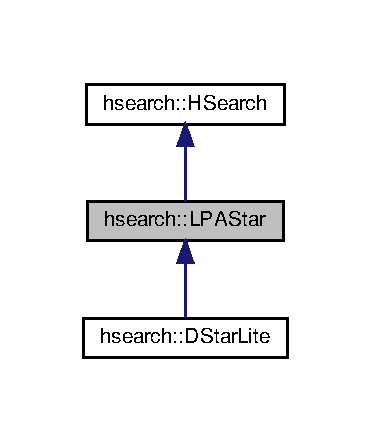
\includegraphics[width=178pt]{d5/da1/classhsearch_1_1LPAStar__inherit__graph}
\end{center}
\end{figure}


Collaboration diagram for hsearch\+:\+:L\+P\+A\+Star\+:
\nopagebreak
\begin{figure}[H]
\begin{center}
\leavevmode
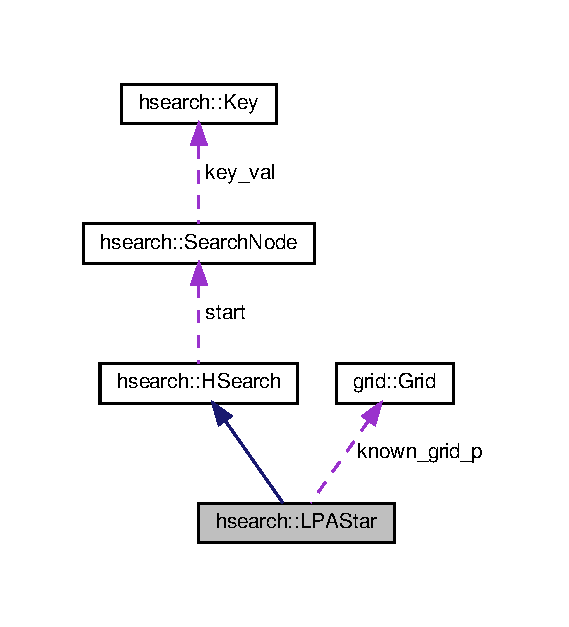
\includegraphics[width=273pt]{dd/d4d/classhsearch_1_1LPAStar__coll__graph}
\end{center}
\end{figure}
\subsection*{Public Member Functions}
\begin{DoxyCompactItemize}
\item 
\mbox{\Hypertarget{classhsearch_1_1LPAStar_accb9219b8a08ab651d3d629a29c281a5}\label{classhsearch_1_1LPAStar_accb9219b8a08ab651d3d629a29c281a5}} 
\hyperlink{classhsearch_1_1LPAStar_accb9219b8a08ab651d3d629a29c281a5}{L\+P\+A\+Star} ()
\begin{DoxyCompactList}\small\item\em Default Constructor. \end{DoxyCompactList}\item 
\hyperlink{classhsearch_1_1LPAStar_a4272517c63ee82c3b745cbaaa0b98a59}{L\+P\+A\+Star} (std\+::vector$<$ std\+::vector$<$ \hyperlink{structprm_1_1Node}{prm\+::\+Node} $>$$>$ $\ast$grid\+\_\+graph, \hyperlink{classgrid_1_1Grid}{grid\+::\+Grid} $\ast$base\+\_\+grid, rigid2d\+::\+Vector2D start\+\_\+loc, rigid2d\+::\+Vector2D \hyperlink{classhsearch_1_1HSearch_a201d281d6a8d9fcc4158772f862d1847}{goal\+\_\+loc})
\begin{DoxyCompactList}\small\item\em provide the search with the beginning state of the map \end{DoxyCompactList}\item 
bool \hyperlink{classhsearch_1_1LPAStar_abccf3f72259c5311b62ffbfdf78a3de4}{Compute\+Shortest\+Path} ()
\begin{DoxyCompactList}\small\item\em The main loop for to find the shortest path. \end{DoxyCompactList}\item 
bool \hyperlink{classhsearch_1_1LPAStar_ad5ba304f7a500b285d4878ee2090f7c3}{Map\+Change} (std\+::vector$<$ std\+::pair$<$ rigid2d\+::\+Vector2D, signed char $>$$>$ points)
\begin{DoxyCompactList}\small\item\em Take in simulated sensor information and determine if there is a change in the map. \end{DoxyCompactList}\end{DoxyCompactItemize}
\subsection*{Protected Member Functions}
\begin{DoxyCompactItemize}
\item 
void \hyperlink{classhsearch_1_1LPAStar_aae9f9031efbe788a83f842905b63e2aa}{assemble\+\_\+path} (\hyperlink{structhsearch_1_1SearchNode}{Search\+Node} goal)
\begin{DoxyCompactList}\small\item\em build the final path based on all of the saved pointers \end{DoxyCompactList}\item 
void \hyperlink{classhsearch_1_1LPAStar_a41219de9a23ffe245589dc34a35e0639}{Update\+Vertex} (int u)
\begin{DoxyCompactList}\small\item\em Update a node. \end{DoxyCompactList}\item 
void \hyperlink{classhsearch_1_1LPAStar_aaeb55f7d05b4952247e492a7db18438d}{Compute\+Cost} (\hyperlink{structhsearch_1_1SearchNode}{Search\+Node} \&s, \hyperlink{structhsearch_1_1SearchNode}{Search\+Node} \&sp)
\begin{DoxyCompactList}\small\item\em a function used to compute the cost for a pair of nodes \end{DoxyCompactList}\item 
double \hyperlink{classhsearch_1_1LPAStar_a92e2fda4e5b1f8ab77297d8cd45e56a7}{edge\+\_\+cost} (\hyperlink{structhsearch_1_1SearchNode}{Search\+Node} \&s, \hyperlink{structhsearch_1_1SearchNode}{Search\+Node} \&sp)
\begin{DoxyCompactList}\small\item\em a function used calculate traversal cost between 2 nodes based on the known\+\_\+map. Uses the stored point in each node to determine if a cell is free or occupied. If one is occupied the cost is set to H\+U\+G\+E\+\_\+\+V\+AL, otherwise use the straight line distance. \end{DoxyCompactList}\item 
\hyperlink{structhsearch_1_1SearchNode}{Search\+Node} $\ast$ \hyperlink{classhsearch_1_1LPAStar_ad5b74c1a38d9db460324fcb1784ac114}{locate\+\_\+node} (int u\+\_\+id)
\begin{DoxyCompactList}\small\item\em Locate a node in the open list or standby. \end{DoxyCompactList}\item 
\hyperlink{structhsearch_1_1Key}{Key} \hyperlink{classhsearch_1_1LPAStar_abffa3312bfb076a9c48ca40de32ec9b2}{get\+\_\+goal\+\_\+key} ()
\begin{DoxyCompactList}\small\item\em Get a reference to the goal node. \end{DoxyCompactList}\item 
bool \hyperlink{classhsearch_1_1LPAStar_a999387c32e95f4b00a9251c5adae4aa5}{goal\+\_\+is\+\_\+consistent} ()
\begin{DoxyCompactList}\small\item\em Check the local consistency of a node. \end{DoxyCompactList}\item 
bool \hyperlink{classhsearch_1_1LPAStar_a034b8a41e91d684932dd014139c4fcd1}{is\+\_\+consistent} (\hyperlink{structhsearch_1_1SearchNode}{Search\+Node} u) const
\begin{DoxyCompactList}\small\item\em Determine if a node is locally is consistent. \end{DoxyCompactList}\end{DoxyCompactItemize}
\subsection*{Protected Attributes}
\begin{DoxyCompactItemize}
\item 
\mbox{\Hypertarget{classhsearch_1_1LPAStar_a75e7bdc0841fd31468c41a58ac842aed}\label{classhsearch_1_1LPAStar_a75e7bdc0841fd31468c41a58ac842aed}} 
std\+::vector$<$ std\+::vector$<$ \hyperlink{structprm_1_1Node}{prm\+::\+Node} $>$ $>$ $\ast$ \hyperlink{classhsearch_1_1LPAStar_a75e7bdc0841fd31468c41a58ac842aed}{created\+\_\+graph\+\_\+p}
\begin{DoxyCompactList}\small\item\em pointer to a 2D vector of created nodes \end{DoxyCompactList}\item 
\mbox{\Hypertarget{classhsearch_1_1LPAStar_ad96878a72794979745566de57b9a361d}\label{classhsearch_1_1LPAStar_ad96878a72794979745566de57b9a361d}} 
\hyperlink{classgrid_1_1Grid}{grid\+::\+Grid} $\ast$ \hyperlink{classhsearch_1_1LPAStar_ad96878a72794979745566de57b9a361d}{known\+\_\+grid\+\_\+p}
\begin{DoxyCompactList}\small\item\em pointer to the known grid containing current occupancy data \end{DoxyCompactList}\item 
\mbox{\Hypertarget{classhsearch_1_1LPAStar_afb7587e07b8f73ecc5edef922924d1bf}\label{classhsearch_1_1LPAStar_afb7587e07b8f73ecc5edef922924d1bf}} 
std\+::unordered\+\_\+map$<$ int, \hyperlink{structhsearch_1_1SearchNode}{Search\+Node} $>$ \hyperlink{classhsearch_1_1LPAStar_afb7587e07b8f73ecc5edef922924d1bf}{standby}
\begin{DoxyCompactList}\small\item\em all nodes not on the open list \end{DoxyCompactList}\item 
\mbox{\Hypertarget{classhsearch_1_1LPAStar_a58cdedcd572ecccbddb30e5d0fc4deab}\label{classhsearch_1_1LPAStar_a58cdedcd572ecccbddb30e5d0fc4deab}} 
int \hyperlink{classhsearch_1_1LPAStar_a58cdedcd572ecccbddb30e5d0fc4deab}{start\+\_\+id}
\begin{DoxyCompactList}\small\item\em ID of the \hyperlink{structhsearch_1_1SearchNode}{Search\+Node} conttaining the start of the search. \end{DoxyCompactList}\item 
\mbox{\Hypertarget{classhsearch_1_1LPAStar_a5788af90341b229108706b497cdf24ae}\label{classhsearch_1_1LPAStar_a5788af90341b229108706b497cdf24ae}} 
int \hyperlink{classhsearch_1_1LPAStar_a5788af90341b229108706b497cdf24ae}{goal\+\_\+id}
\begin{DoxyCompactList}\small\item\em ID of the \hyperlink{structhsearch_1_1SearchNode}{Search\+Node} conttaining the goal of the search. \end{DoxyCompactList}\item 
\mbox{\Hypertarget{classhsearch_1_1LPAStar_a8da37ca2b4be6ad6a64f38827fab3545}\label{classhsearch_1_1LPAStar_a8da37ca2b4be6ad6a64f38827fab3545}} 
double \hyperlink{classhsearch_1_1LPAStar_a8da37ca2b4be6ad6a64f38827fab3545}{km} = 0
\begin{DoxyCompactList}\small\item\em \hyperlink{structhsearch_1_1Key}{Key} modifier used by D$\ast$ Lite. \end{DoxyCompactList}\end{DoxyCompactItemize}


\subsection{Detailed Description}
a class to perform L\+P\+A$\ast$ search 

\subsection{Constructor \& Destructor Documentation}
\mbox{\Hypertarget{classhsearch_1_1LPAStar_a4272517c63ee82c3b745cbaaa0b98a59}\label{classhsearch_1_1LPAStar_a4272517c63ee82c3b745cbaaa0b98a59}} 
\index{hsearch\+::\+L\+P\+A\+Star@{hsearch\+::\+L\+P\+A\+Star}!L\+P\+A\+Star@{L\+P\+A\+Star}}
\index{L\+P\+A\+Star@{L\+P\+A\+Star}!hsearch\+::\+L\+P\+A\+Star@{hsearch\+::\+L\+P\+A\+Star}}
\subsubsection{\texorpdfstring{L\+P\+A\+Star()}{LPAStar()}}
{\footnotesize\ttfamily hsearch\+::\+L\+P\+A\+Star\+::\+L\+P\+A\+Star (\begin{DoxyParamCaption}\item[{std\+::vector$<$ std\+::vector$<$ \hyperlink{structprm_1_1Node}{prm\+::\+Node} $>$$>$ $\ast$}]{grid\+\_\+graph,  }\item[{\hyperlink{classgrid_1_1Grid}{grid\+::\+Grid} $\ast$}]{base\+\_\+grid,  }\item[{rigid2d\+::\+Vector2D}]{start\+\_\+loc,  }\item[{rigid2d\+::\+Vector2D}]{goal\+\_\+loc }\end{DoxyParamCaption})}



provide the search with the beginning state of the map 


\begin{DoxyParams}{Parameters}
{\em grid\+\_\+graph} & reference to an existing grid \\
\hline
{\em base\+\_\+grid} & pointer to the Grid the search is using \\
\hline
{\em start\+\_\+loc} & the location of the starting point in integer coordinates on the provided grid \\
\hline
{\em goal\+\_\+loc} & the location of the goal point in integer coordinates on the provided grid \\
\hline
\end{DoxyParams}


\subsection{Member Function Documentation}
\mbox{\Hypertarget{classhsearch_1_1LPAStar_aae9f9031efbe788a83f842905b63e2aa}\label{classhsearch_1_1LPAStar_aae9f9031efbe788a83f842905b63e2aa}} 
\index{hsearch\+::\+L\+P\+A\+Star@{hsearch\+::\+L\+P\+A\+Star}!assemble\+\_\+path@{assemble\+\_\+path}}
\index{assemble\+\_\+path@{assemble\+\_\+path}!hsearch\+::\+L\+P\+A\+Star@{hsearch\+::\+L\+P\+A\+Star}}
\subsubsection{\texorpdfstring{assemble\+\_\+path()}{assemble\_path()}}
{\footnotesize\ttfamily void hsearch\+::\+L\+P\+A\+Star\+::assemble\+\_\+path (\begin{DoxyParamCaption}\item[{\hyperlink{structhsearch_1_1SearchNode}{Search\+Node}}]{goal }\end{DoxyParamCaption})\hspace{0.3cm}{\ttfamily [protected]}, {\ttfamily [virtual]}}



build the final path based on all of the saved pointers 


\begin{DoxyParams}{Parameters}
{\em goal} & the goal \hyperlink{structhsearch_1_1SearchNode}{Search\+Node} \\
\hline
\end{DoxyParams}


Reimplemented from \hyperlink{classhsearch_1_1HSearch_ac94c08c0f0d4cc3076f01d70c6cd7679}{hsearch\+::\+H\+Search}.

\mbox{\Hypertarget{classhsearch_1_1LPAStar_aaeb55f7d05b4952247e492a7db18438d}\label{classhsearch_1_1LPAStar_aaeb55f7d05b4952247e492a7db18438d}} 
\index{hsearch\+::\+L\+P\+A\+Star@{hsearch\+::\+L\+P\+A\+Star}!Compute\+Cost@{Compute\+Cost}}
\index{Compute\+Cost@{Compute\+Cost}!hsearch\+::\+L\+P\+A\+Star@{hsearch\+::\+L\+P\+A\+Star}}
\subsubsection{\texorpdfstring{Compute\+Cost()}{ComputeCost()}}
{\footnotesize\ttfamily void hsearch\+::\+L\+P\+A\+Star\+::\+Compute\+Cost (\begin{DoxyParamCaption}\item[{\hyperlink{structhsearch_1_1SearchNode}{Search\+Node} \&}]{s,  }\item[{\hyperlink{structhsearch_1_1SearchNode}{Search\+Node} \&}]{sp }\end{DoxyParamCaption})\hspace{0.3cm}{\ttfamily [protected]}, {\ttfamily [virtual]}}



a function used to compute the cost for a pair of nodes 


\begin{DoxyParams}{Parameters}
{\em s} & the current node being expanded \\
\hline
{\em sp} & the neighbor node being evaluated \\
\hline
\end{DoxyParams}


Implements \hyperlink{classhsearch_1_1HSearch_a5d325955c4faedaca0c68155fd1f7e69}{hsearch\+::\+H\+Search}.

\mbox{\Hypertarget{classhsearch_1_1LPAStar_abccf3f72259c5311b62ffbfdf78a3de4}\label{classhsearch_1_1LPAStar_abccf3f72259c5311b62ffbfdf78a3de4}} 
\index{hsearch\+::\+L\+P\+A\+Star@{hsearch\+::\+L\+P\+A\+Star}!Compute\+Shortest\+Path@{Compute\+Shortest\+Path}}
\index{Compute\+Shortest\+Path@{Compute\+Shortest\+Path}!hsearch\+::\+L\+P\+A\+Star@{hsearch\+::\+L\+P\+A\+Star}}
\subsubsection{\texorpdfstring{Compute\+Shortest\+Path()}{ComputeShortestPath()}}
{\footnotesize\ttfamily bool hsearch\+::\+L\+P\+A\+Star\+::\+Compute\+Shortest\+Path (\begin{DoxyParamCaption}{ }\end{DoxyParamCaption})}



The main loop for to find the shortest path. 

\begin{DoxyReturn}{Returns}
True if a path was found, otherwise False 
\end{DoxyReturn}
\mbox{\Hypertarget{classhsearch_1_1LPAStar_a92e2fda4e5b1f8ab77297d8cd45e56a7}\label{classhsearch_1_1LPAStar_a92e2fda4e5b1f8ab77297d8cd45e56a7}} 
\index{hsearch\+::\+L\+P\+A\+Star@{hsearch\+::\+L\+P\+A\+Star}!edge\+\_\+cost@{edge\+\_\+cost}}
\index{edge\+\_\+cost@{edge\+\_\+cost}!hsearch\+::\+L\+P\+A\+Star@{hsearch\+::\+L\+P\+A\+Star}}
\subsubsection{\texorpdfstring{edge\+\_\+cost()}{edge\_cost()}}
{\footnotesize\ttfamily double hsearch\+::\+L\+P\+A\+Star\+::edge\+\_\+cost (\begin{DoxyParamCaption}\item[{\hyperlink{structhsearch_1_1SearchNode}{Search\+Node} \&}]{s,  }\item[{\hyperlink{structhsearch_1_1SearchNode}{Search\+Node} \&}]{sp }\end{DoxyParamCaption})\hspace{0.3cm}{\ttfamily [protected]}}



a function used calculate traversal cost between 2 nodes based on the known\+\_\+map. Uses the stored point in each node to determine if a cell is free or occupied. If one is occupied the cost is set to H\+U\+G\+E\+\_\+\+V\+AL, otherwise use the straight line distance. 


\begin{DoxyParams}{Parameters}
{\em s} & the current node being expanded \\
\hline
{\em sp} & the neighbor node being evaluated \\
\hline
\end{DoxyParams}
\begin{DoxyReturn}{Returns}
the cost to traverse from sp to s 
\end{DoxyReturn}
\mbox{\Hypertarget{classhsearch_1_1LPAStar_abffa3312bfb076a9c48ca40de32ec9b2}\label{classhsearch_1_1LPAStar_abffa3312bfb076a9c48ca40de32ec9b2}} 
\index{hsearch\+::\+L\+P\+A\+Star@{hsearch\+::\+L\+P\+A\+Star}!get\+\_\+goal\+\_\+key@{get\+\_\+goal\+\_\+key}}
\index{get\+\_\+goal\+\_\+key@{get\+\_\+goal\+\_\+key}!hsearch\+::\+L\+P\+A\+Star@{hsearch\+::\+L\+P\+A\+Star}}
\subsubsection{\texorpdfstring{get\+\_\+goal\+\_\+key()}{get\_goal\_key()}}
{\footnotesize\ttfamily \hyperlink{structhsearch_1_1Key}{Key} hsearch\+::\+L\+P\+A\+Star\+::get\+\_\+goal\+\_\+key (\begin{DoxyParamCaption}{ }\end{DoxyParamCaption})\hspace{0.3cm}{\ttfamily [protected]}}



Get a reference to the goal node. 

\begin{DoxyReturn}{Returns}
goal key 
\end{DoxyReturn}
\mbox{\Hypertarget{classhsearch_1_1LPAStar_a999387c32e95f4b00a9251c5adae4aa5}\label{classhsearch_1_1LPAStar_a999387c32e95f4b00a9251c5adae4aa5}} 
\index{hsearch\+::\+L\+P\+A\+Star@{hsearch\+::\+L\+P\+A\+Star}!goal\+\_\+is\+\_\+consistent@{goal\+\_\+is\+\_\+consistent}}
\index{goal\+\_\+is\+\_\+consistent@{goal\+\_\+is\+\_\+consistent}!hsearch\+::\+L\+P\+A\+Star@{hsearch\+::\+L\+P\+A\+Star}}
\subsubsection{\texorpdfstring{goal\+\_\+is\+\_\+consistent()}{goal\_is\_consistent()}}
{\footnotesize\ttfamily bool hsearch\+::\+L\+P\+A\+Star\+::goal\+\_\+is\+\_\+consistent (\begin{DoxyParamCaption}{ }\end{DoxyParamCaption})\hspace{0.3cm}{\ttfamily [protected]}}



Check the local consistency of a node. 

\begin{DoxyReturn}{Returns}
true if the goal is locally consistent, otherwise false 
\end{DoxyReturn}
\mbox{\Hypertarget{classhsearch_1_1LPAStar_a034b8a41e91d684932dd014139c4fcd1}\label{classhsearch_1_1LPAStar_a034b8a41e91d684932dd014139c4fcd1}} 
\index{hsearch\+::\+L\+P\+A\+Star@{hsearch\+::\+L\+P\+A\+Star}!is\+\_\+consistent@{is\+\_\+consistent}}
\index{is\+\_\+consistent@{is\+\_\+consistent}!hsearch\+::\+L\+P\+A\+Star@{hsearch\+::\+L\+P\+A\+Star}}
\subsubsection{\texorpdfstring{is\+\_\+consistent()}{is\_consistent()}}
{\footnotesize\ttfamily bool hsearch\+::\+L\+P\+A\+Star\+::is\+\_\+consistent (\begin{DoxyParamCaption}\item[{\hyperlink{structhsearch_1_1SearchNode}{Search\+Node}}]{u }\end{DoxyParamCaption}) const\hspace{0.3cm}{\ttfamily [protected]}}



Determine if a node is locally is consistent. 


\begin{DoxyParams}{Parameters}
{\em u} & a node to evaluate \\
\hline
\end{DoxyParams}
\begin{DoxyReturn}{Returns}
True if the node is locally consistent 
\end{DoxyReturn}
\mbox{\Hypertarget{classhsearch_1_1LPAStar_ad5b74c1a38d9db460324fcb1784ac114}\label{classhsearch_1_1LPAStar_ad5b74c1a38d9db460324fcb1784ac114}} 
\index{hsearch\+::\+L\+P\+A\+Star@{hsearch\+::\+L\+P\+A\+Star}!locate\+\_\+node@{locate\+\_\+node}}
\index{locate\+\_\+node@{locate\+\_\+node}!hsearch\+::\+L\+P\+A\+Star@{hsearch\+::\+L\+P\+A\+Star}}
\subsubsection{\texorpdfstring{locate\+\_\+node()}{locate\_node()}}
{\footnotesize\ttfamily \hyperlink{structhsearch_1_1SearchNode}{Search\+Node} $\ast$ hsearch\+::\+L\+P\+A\+Star\+::locate\+\_\+node (\begin{DoxyParamCaption}\item[{int}]{u\+\_\+id }\end{DoxyParamCaption})\hspace{0.3cm}{\ttfamily [protected]}}



Locate a node in the open list or standby. 


\begin{DoxyParams}{Parameters}
{\em u\+\_\+id} & the id of a node to find \\
\hline
\end{DoxyParams}
\begin{DoxyReturn}{Returns}
a pointer to the node 
\end{DoxyReturn}
\mbox{\Hypertarget{classhsearch_1_1LPAStar_ad5ba304f7a500b285d4878ee2090f7c3}\label{classhsearch_1_1LPAStar_ad5ba304f7a500b285d4878ee2090f7c3}} 
\index{hsearch\+::\+L\+P\+A\+Star@{hsearch\+::\+L\+P\+A\+Star}!Map\+Change@{Map\+Change}}
\index{Map\+Change@{Map\+Change}!hsearch\+::\+L\+P\+A\+Star@{hsearch\+::\+L\+P\+A\+Star}}
\subsubsection{\texorpdfstring{Map\+Change()}{MapChange()}}
{\footnotesize\ttfamily bool hsearch\+::\+L\+P\+A\+Star\+::\+Map\+Change (\begin{DoxyParamCaption}\item[{std\+::vector$<$ std\+::pair$<$ rigid2d\+::\+Vector2D, signed char $>$$>$}]{points }\end{DoxyParamCaption})}



Take in simulated sensor information and determine if there is a change in the map. 


\begin{DoxyParams}{Parameters}
{\em points} & pairs of grid cell locations and new occupancy data to potentially update. \\
\hline
\end{DoxyParams}
\begin{DoxyReturn}{Returns}
True if the information in points actually caused a change in the occupancy data from free to occupied, otherwise False. 
\end{DoxyReturn}
\mbox{\Hypertarget{classhsearch_1_1LPAStar_a41219de9a23ffe245589dc34a35e0639}\label{classhsearch_1_1LPAStar_a41219de9a23ffe245589dc34a35e0639}} 
\index{hsearch\+::\+L\+P\+A\+Star@{hsearch\+::\+L\+P\+A\+Star}!Update\+Vertex@{Update\+Vertex}}
\index{Update\+Vertex@{Update\+Vertex}!hsearch\+::\+L\+P\+A\+Star@{hsearch\+::\+L\+P\+A\+Star}}
\subsubsection{\texorpdfstring{Update\+Vertex()}{UpdateVertex()}}
{\footnotesize\ttfamily void hsearch\+::\+L\+P\+A\+Star\+::\+Update\+Vertex (\begin{DoxyParamCaption}\item[{int}]{u }\end{DoxyParamCaption})\hspace{0.3cm}{\ttfamily [protected]}}



Update a node. 


\begin{DoxyParams}{Parameters}
{\em u} & the id of a node to update \\
\hline
\end{DoxyParams}


The documentation for this class was generated from the following files\+:\begin{DoxyCompactItemize}
\item 
global\+\_\+search/include/global\+\_\+search/\hyperlink{heuristic__search_8hpp}{heuristic\+\_\+search.\+hpp}\item 
global\+\_\+search/src/global\+\_\+search/\hyperlink{heuristic__search_8cpp}{heuristic\+\_\+search.\+cpp}\end{DoxyCompactItemize}

\hypertarget{structgrid_1_1Map}{}\section{grid\+:\+:Map Struct Reference}
\label{structgrid_1_1Map}\index{grid\+::\+Map@{grid\+::\+Map}}


Contains information about a bound map.  




{\ttfamily \#include $<$grid.\+hpp$>$}

\subsection*{Public Member Functions}
\begin{DoxyCompactItemize}
\item 
\mbox{\Hypertarget{structgrid_1_1Map_aeedaf34b4dcd443691c796637cea73ce}\label{structgrid_1_1Map_aeedaf34b4dcd443691c796637cea73ce}} 
\hyperlink{structgrid_1_1Map_aeedaf34b4dcd443691c796637cea73ce}{Map} ()
\begin{DoxyCompactList}\small\item\em default constructor \end{DoxyCompactList}\item 
\hyperlink{structgrid_1_1Map_a124140efcef69cee1d90f5d81d01e8fa}{Map} (std\+::vector$<$ std\+::vector$<$ rigid2d\+::\+Vector2D $>$$>$ obs, std\+::vector$<$ double $>$ x, std\+::vector$<$ double $>$ y)
\begin{DoxyCompactList}\small\item\em Fully construct the map. \end{DoxyCompactList}\end{DoxyCompactItemize}
\subsection*{Public Attributes}
\begin{DoxyCompactItemize}
\item 
\mbox{\Hypertarget{structgrid_1_1Map_ab9f49bab16cb300a8de972a412c54375}\label{structgrid_1_1Map_ab9f49bab16cb300a8de972a412c54375}} 
std\+::vector$<$ std\+::vector$<$ rigid2d\+::\+Vector2D $>$ $>$ \hyperlink{structgrid_1_1Map_ab9f49bab16cb300a8de972a412c54375}{obstacles}
\begin{DoxyCompactList}\small\item\em obstacles in the map \end{DoxyCompactList}\item 
\mbox{\Hypertarget{structgrid_1_1Map_a44918e798d8fa1400ddf52bc52ce4c6f}\label{structgrid_1_1Map_a44918e798d8fa1400ddf52bc52ce4c6f}} 
std\+::vector$<$ double $>$ \hyperlink{structgrid_1_1Map_a44918e798d8fa1400ddf52bc52ce4c6f}{x\+\_\+bounds}
\begin{DoxyCompactList}\small\item\em x bounds of the map \end{DoxyCompactList}\item 
\mbox{\Hypertarget{structgrid_1_1Map_a5f51eeac70566244a15c1023e9f494fb}\label{structgrid_1_1Map_a5f51eeac70566244a15c1023e9f494fb}} 
std\+::vector$<$ double $>$ \hyperlink{structgrid_1_1Map_a5f51eeac70566244a15c1023e9f494fb}{y\+\_\+bounds}
\begin{DoxyCompactList}\small\item\em y bounds of the map \end{DoxyCompactList}\item 
\mbox{\Hypertarget{structgrid_1_1Map_a5ee687d67cff44b8e447b2b92603056b}\label{structgrid_1_1Map_a5ee687d67cff44b8e447b2b92603056b}} 
std\+::vector$<$ rigid2d\+::\+Vector2D $>$ \hyperlink{structgrid_1_1Map_a5ee687d67cff44b8e447b2b92603056b}{map\+\_\+vector}
\begin{DoxyCompactList}\small\item\em a vector of the map verticies in ccw order \end{DoxyCompactList}\end{DoxyCompactItemize}


\subsection{Detailed Description}
Contains information about a bound map. 

\subsection{Constructor \& Destructor Documentation}
\mbox{\Hypertarget{structgrid_1_1Map_a124140efcef69cee1d90f5d81d01e8fa}\label{structgrid_1_1Map_a124140efcef69cee1d90f5d81d01e8fa}} 
\index{grid\+::\+Map@{grid\+::\+Map}!Map@{Map}}
\index{Map@{Map}!grid\+::\+Map@{grid\+::\+Map}}
\subsubsection{\texorpdfstring{Map()}{Map()}}
{\footnotesize\ttfamily grid\+::\+Map\+::\+Map (\begin{DoxyParamCaption}\item[{std\+::vector$<$ std\+::vector$<$ rigid2d\+::\+Vector2D $>$$>$}]{obs,  }\item[{std\+::vector$<$ double $>$}]{x,  }\item[{std\+::vector$<$ double $>$}]{y }\end{DoxyParamCaption})}



Fully construct the map. 


\begin{DoxyParams}{Parameters}
{\em obs} & obstacles in the map \\
\hline
{\em x} & bounds of the map \\
\hline
{\em y} & bounds of the map \\
\hline
\end{DoxyParams}


The documentation for this struct was generated from the following files\+:\begin{DoxyCompactItemize}
\item 
roadmap/include/roadmap/grid.\+hpp\item 
roadmap/src/roadmap/grid.\+cpp\end{DoxyCompactItemize}

\hypertarget{structprm_1_1Node}{}\section{prm\+:\+:Node Struct Reference}
\label{structprm_1_1Node}\index{prm\+::\+Node@{prm\+::\+Node}}


A struct to define a node and interact with it.  




{\ttfamily \#include $<$prm.\+hpp$>$}

\subsection*{Public Member Functions}
\begin{DoxyCompactItemize}
\item 
bool \hyperlink{structprm_1_1Node_a166ab395f8fcb59f5d5367ca45f7bf51}{Is\+Connected} (int node\+\_\+id) const
\begin{DoxyCompactList}\small\item\em Determine if a node is connected to this one. \end{DoxyCompactList}\item 
bool \hyperlink{structprm_1_1Node_ad414f13a52664be229be3a594613fb45}{operator$<$} (const \hyperlink{structprm_1_1Node}{Node} \&rhs) const
\begin{DoxyCompactList}\small\item\em Compares the distance value of this node object and another. \end{DoxyCompactList}\end{DoxyCompactItemize}
\subsection*{Public Attributes}
\begin{DoxyCompactItemize}
\item 
\mbox{\Hypertarget{structprm_1_1Node_a538d85b9f504bdb39268bd3168fd9211}\label{structprm_1_1Node_a538d85b9f504bdb39268bd3168fd9211}} 
int \hyperlink{structprm_1_1Node_a538d85b9f504bdb39268bd3168fd9211}{id} = -\/1
\begin{DoxyCompactList}\small\item\em unique node ID \end{DoxyCompactList}\item 
\mbox{\Hypertarget{structprm_1_1Node_afcf2b1941863d8d9a60874a30b9d2938}\label{structprm_1_1Node_afcf2b1941863d8d9a60874a30b9d2938}} 
rigid2d\+::\+Vector2D \hyperlink{structprm_1_1Node_afcf2b1941863d8d9a60874a30b9d2938}{point}
\begin{DoxyCompactList}\small\item\em x,y location relative to the world \end{DoxyCompactList}\item 
\mbox{\Hypertarget{structprm_1_1Node_abf983b6e36e98f9caf0766b1e8c5500a}\label{structprm_1_1Node_abf983b6e36e98f9caf0766b1e8c5500a}} 
std\+::vector$<$ \hyperlink{structprm_1_1Edge}{Edge} $>$ \hyperlink{structprm_1_1Node_abf983b6e36e98f9caf0766b1e8c5500a}{edges}
\begin{DoxyCompactList}\small\item\em edges connecting to nearby nodes \end{DoxyCompactList}\item 
\mbox{\Hypertarget{structprm_1_1Node_a23d5570a4b85f7403399444e68d5aa52}\label{structprm_1_1Node_a23d5570a4b85f7403399444e68d5aa52}} 
std\+::unordered\+\_\+set$<$ int $>$ \hyperlink{structprm_1_1Node_a23d5570a4b85f7403399444e68d5aa52}{id\+\_\+set}
\begin{DoxyCompactList}\small\item\em nodes that should be connected \end{DoxyCompactList}\item 
\mbox{\Hypertarget{structprm_1_1Node_af137867e3fb1f9b0d3e43ef3fd8ddecd}\label{structprm_1_1Node_af137867e3fb1f9b0d3e43ef3fd8ddecd}} 
double \hyperlink{structprm_1_1Node_af137867e3fb1f9b0d3e43ef3fd8ddecd}{weight} = 0
\begin{DoxyCompactList}\small\item\em weight to determine if map is properly sampled \end{DoxyCompactList}\item 
\mbox{\Hypertarget{structprm_1_1Node_a4db5966bcf026eaa4f2cd07ea22bcb4f}\label{structprm_1_1Node_a4db5966bcf026eaa4f2cd07ea22bcb4f}} 
double \hyperlink{structprm_1_1Node_a4db5966bcf026eaa4f2cd07ea22bcb4f}{distance} =0
\begin{DoxyCompactList}\small\item\em the distance to a node, used to find k-\/nearest nodes \end{DoxyCompactList}\end{DoxyCompactItemize}


\subsection{Detailed Description}
A struct to define a node and interact with it. 

\subsection{Member Function Documentation}
\mbox{\Hypertarget{structprm_1_1Node_a166ab395f8fcb59f5d5367ca45f7bf51}\label{structprm_1_1Node_a166ab395f8fcb59f5d5367ca45f7bf51}} 
\index{prm\+::\+Node@{prm\+::\+Node}!Is\+Connected@{Is\+Connected}}
\index{Is\+Connected@{Is\+Connected}!prm\+::\+Node@{prm\+::\+Node}}
\subsubsection{\texorpdfstring{Is\+Connected()}{IsConnected()}}
{\footnotesize\ttfamily bool prm\+::\+Node\+::\+Is\+Connected (\begin{DoxyParamCaption}\item[{int}]{node\+\_\+id }\end{DoxyParamCaption}) const\hspace{0.3cm}{\ttfamily [inline]}}



Determine if a node is connected to this one. 


\begin{DoxyParams}{Parameters}
{\em node\+\_\+id} & ID to check for a connection \\
\hline
\end{DoxyParams}
\begin{DoxyReturn}{Returns}
True if a connection exists 
\end{DoxyReturn}
\mbox{\Hypertarget{structprm_1_1Node_ad414f13a52664be229be3a594613fb45}\label{structprm_1_1Node_ad414f13a52664be229be3a594613fb45}} 
\index{prm\+::\+Node@{prm\+::\+Node}!operator$<$@{operator$<$}}
\index{operator$<$@{operator$<$}!prm\+::\+Node@{prm\+::\+Node}}
\subsubsection{\texorpdfstring{operator$<$()}{operator<()}}
{\footnotesize\ttfamily bool prm\+::\+Node\+::operator$<$ (\begin{DoxyParamCaption}\item[{const \hyperlink{structprm_1_1Node}{Node} \&}]{rhs }\end{DoxyParamCaption}) const\hspace{0.3cm}{\ttfamily [inline]}}



Compares the distance value of this node object and another. 


\begin{DoxyParams}{Parameters}
{\em rhs} & pointer to another node object \\
\hline
\end{DoxyParams}
\begin{DoxyReturn}{Returns}
True if this node has a smaller distance 
\end{DoxyReturn}


The documentation for this struct was generated from the following file\+:\begin{DoxyCompactItemize}
\item 
roadmap/include/roadmap/\hyperlink{prm_8hpp}{prm.\+hpp}\end{DoxyCompactItemize}

\hypertarget{classpfield_1_1PtField}{}\section{pfield\+:\+:Pt\+Field Class Reference}
\label{classpfield_1_1PtField}\index{pfield\+::\+Pt\+Field@{pfield\+::\+Pt\+Field}}


brief class to allow planning  




{\ttfamily \#include $<$potential\+\_\+fields.\+hpp$>$}



Collaboration diagram for pfield\+:\+:Pt\+Field\+:\nopagebreak
\begin{figure}[H]
\begin{center}
\leavevmode
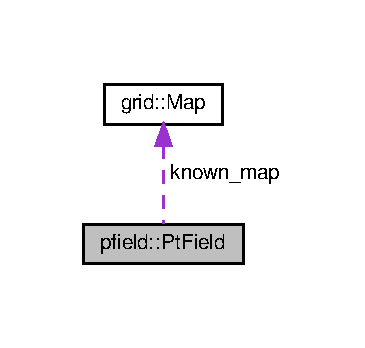
\includegraphics[width=175pt]{df/d59/classpfield_1_1PtField__coll__graph}
\end{center}
\end{figure}
\subsection*{Public Member Functions}
\begin{DoxyCompactItemize}
\item 
\hyperlink{classpfield_1_1PtField_aee7dcc713ac6d16364e8bebe2da64681}{Pt\+Field} (\hyperlink{structgrid_1_1Map}{grid\+::\+Map} map, rigid2d\+::\+Vector2D goal, double z, double aw, double dg, double rw, double Qs)
\begin{DoxyCompactList}\small\item\em constuctor to initialize the Potential Field Planner \end{DoxyCompactList}\item 
rigid2d\+::\+Vector2D \hyperlink{classpfield_1_1PtField_af1faea5a1127d6df5e06727391227ade}{Plan\+One\+Step} (rigid2d\+::\+Vector2D cur\+\_\+loc)
\begin{DoxyCompactList}\small\item\em given the robots location, plan its next step \end{DoxyCompactList}\item 
std\+::vector$<$ rigid2d\+::\+Vector2D $>$ \hyperlink{classpfield_1_1PtField_ab936f2bf686f45a2a11825e5a8911356}{get\+\_\+path} ()
\begin{DoxyCompactList}\small\item\em retrieve the whole planned path \end{DoxyCompactList}\end{DoxyCompactItemize}
\subsection*{Private Member Functions}
\begin{DoxyCompactItemize}
\item 
rigid2d\+::\+Vector2D \hyperlink{classpfield_1_1PtField_a1cbfedd08d4e271264f10e5b5c9b57bd}{calculate\+\_\+u\+\_\+att} (rigid2d\+::\+Vector2D cur\+\_\+loc)
\begin{DoxyCompactList}\small\item\em Calculate the attractive component of the \char`\"{}force\char`\"{} based on the distance to goal. \end{DoxyCompactList}\item 
rigid2d\+::\+Vector2D \hyperlink{classpfield_1_1PtField_a8d47de5b4a724e2100c70676e683298b}{calculate\+\_\+u\+\_\+rep} (rigid2d\+::\+Vector2D cur\+\_\+loc)
\begin{DoxyCompactList}\small\item\em Calculate the repulsive component of the \char`\"{}force\char`\"{} based on the distance to each obstacle. \end{DoxyCompactList}\item 
rigid2d\+::\+Vector2D \hyperlink{classpfield_1_1PtField_ac8e3ca79a5c7eb3baeaa4b6097df2c8f}{u\+\_\+rep\+\_\+component} (std\+::vector$<$ rigid2d\+::\+Vector2D $>$ polygon, rigid2d\+::\+Vector2D cur\+\_\+loc)
\begin{DoxyCompactList}\small\item\em Calculate the repulsive component due to a given obstacle. \end{DoxyCompactList}\end{DoxyCompactItemize}
\subsection*{Private Attributes}
\begin{DoxyCompactItemize}
\item 
\mbox{\Hypertarget{classpfield_1_1PtField_af42c90549ef5781d7ace3750a64204fb}\label{classpfield_1_1PtField_af42c90549ef5781d7ace3750a64204fb}} 
\hyperlink{structgrid_1_1Map}{grid\+::\+Map} \hyperlink{classpfield_1_1PtField_af42c90549ef5781d7ace3750a64204fb}{known\+\_\+map}
\begin{DoxyCompactList}\small\item\em the known map \end{DoxyCompactList}\item 
\mbox{\Hypertarget{classpfield_1_1PtField_abfa912b088856926772dc828a5d62671}\label{classpfield_1_1PtField_abfa912b088856926772dc828a5d62671}} 
rigid2d\+::\+Vector2D \hyperlink{classpfield_1_1PtField_abfa912b088856926772dc828a5d62671}{goal\+\_\+loc}
\begin{DoxyCompactList}\small\item\em the goal location \end{DoxyCompactList}\item 
\mbox{\Hypertarget{classpfield_1_1PtField_a07f90e3a7188276be1f3854f11930c3a}\label{classpfield_1_1PtField_a07f90e3a7188276be1f3854f11930c3a}} 
double \hyperlink{classpfield_1_1PtField_a07f90e3a7188276be1f3854f11930c3a}{zeta}
\begin{DoxyCompactList}\small\item\em the step size for gradient descent \end{DoxyCompactList}\item 
\mbox{\Hypertarget{classpfield_1_1PtField_a43a4e144b8906c64823e872ff270d4c5}\label{classpfield_1_1PtField_a43a4e144b8906c64823e872ff270d4c5}} 
double \hyperlink{classpfield_1_1PtField_a43a4e144b8906c64823e872ff270d4c5}{att\+\_\+weight}
\begin{DoxyCompactList}\small\item\em weighting factor the attactive component \end{DoxyCompactList}\item 
\mbox{\Hypertarget{classpfield_1_1PtField_adadbef461c9255b0c60301508f4cab37}\label{classpfield_1_1PtField_adadbef461c9255b0c60301508f4cab37}} 
double \hyperlink{classpfield_1_1PtField_adadbef461c9255b0c60301508f4cab37}{dg\+\_\+star}
\begin{DoxyCompactList}\small\item\em threshold for piecewise attractive gradient calculation \end{DoxyCompactList}\item 
\mbox{\Hypertarget{classpfield_1_1PtField_acc129742194272617f51b200c49dcd52}\label{classpfield_1_1PtField_acc129742194272617f51b200c49dcd52}} 
double \hyperlink{classpfield_1_1PtField_acc129742194272617f51b200c49dcd52}{rep\+\_\+weight}
\begin{DoxyCompactList}\small\item\em weighting factor the repulsive component \end{DoxyCompactList}\item 
\mbox{\Hypertarget{classpfield_1_1PtField_a1223f43ad697e3539a732b08b5d77926}\label{classpfield_1_1PtField_a1223f43ad697e3539a732b08b5d77926}} 
double \hyperlink{classpfield_1_1PtField_a1223f43ad697e3539a732b08b5d77926}{Qstar}
\begin{DoxyCompactList}\small\item\em threshold for obstacles range of influence \end{DoxyCompactList}\item 
\mbox{\Hypertarget{classpfield_1_1PtField_a941337f34ead9c01f53427075be8a0b9}\label{classpfield_1_1PtField_a941337f34ead9c01f53427075be8a0b9}} 
std\+::vector$<$ rigid2d\+::\+Vector2D $>$ \hyperlink{classpfield_1_1PtField_a941337f34ead9c01f53427075be8a0b9}{final\+\_\+path}
\begin{DoxyCompactList}\small\item\em final path determined \end{DoxyCompactList}\end{DoxyCompactItemize}


\subsection{Detailed Description}
brief class to allow planning 

\subsection{Constructor \& Destructor Documentation}
\mbox{\Hypertarget{classpfield_1_1PtField_aee7dcc713ac6d16364e8bebe2da64681}\label{classpfield_1_1PtField_aee7dcc713ac6d16364e8bebe2da64681}} 
\index{pfield\+::\+Pt\+Field@{pfield\+::\+Pt\+Field}!Pt\+Field@{Pt\+Field}}
\index{Pt\+Field@{Pt\+Field}!pfield\+::\+Pt\+Field@{pfield\+::\+Pt\+Field}}
\subsubsection{\texorpdfstring{Pt\+Field()}{PtField()}}
{\footnotesize\ttfamily pfield\+::\+Pt\+Field\+::\+Pt\+Field (\begin{DoxyParamCaption}\item[{\hyperlink{structgrid_1_1Map}{grid\+::\+Map}}]{map,  }\item[{rigid2d\+::\+Vector2D}]{goal,  }\item[{double}]{z,  }\item[{double}]{aw,  }\item[{double}]{dg,  }\item[{double}]{rw,  }\item[{double}]{Qs }\end{DoxyParamCaption})}



constuctor to initialize the Potential Field Planner 


\begin{DoxyParams}{Parameters}
{\em map} & the known Map \\
\hline
{\em goal} & the x,y location of the goal \\
\hline
{\em z} & the step size for gradient descent \\
\hline
{\em aw} & weighting factor the attactive component \\
\hline
{\em dg} & threshold for piecewise attractive gradient calculation \\
\hline
{\em rw} & weighting factor the repulsive component \\
\hline
{\em Qs} & threshold for obstacles range of influence \\
\hline
\end{DoxyParams}


\subsection{Member Function Documentation}
\mbox{\Hypertarget{classpfield_1_1PtField_a1cbfedd08d4e271264f10e5b5c9b57bd}\label{classpfield_1_1PtField_a1cbfedd08d4e271264f10e5b5c9b57bd}} 
\index{pfield\+::\+Pt\+Field@{pfield\+::\+Pt\+Field}!calculate\+\_\+u\+\_\+att@{calculate\+\_\+u\+\_\+att}}
\index{calculate\+\_\+u\+\_\+att@{calculate\+\_\+u\+\_\+att}!pfield\+::\+Pt\+Field@{pfield\+::\+Pt\+Field}}
\subsubsection{\texorpdfstring{calculate\+\_\+u\+\_\+att()}{calculate\_u\_att()}}
{\footnotesize\ttfamily rigid2d\+::\+Vector2D pfield\+::\+Pt\+Field\+::calculate\+\_\+u\+\_\+att (\begin{DoxyParamCaption}\item[{rigid2d\+::\+Vector2D}]{cur\+\_\+loc }\end{DoxyParamCaption})\hspace{0.3cm}{\ttfamily [private]}}



Calculate the attractive component of the \char`\"{}force\char`\"{} based on the distance to goal. 


\begin{DoxyParams}{Parameters}
{\em cur\+\_\+loc} & the current location of the robot \\
\hline
\end{DoxyParams}
\begin{DoxyReturn}{Returns}
the total attrative gradient 
\end{DoxyReturn}
\mbox{\Hypertarget{classpfield_1_1PtField_a8d47de5b4a724e2100c70676e683298b}\label{classpfield_1_1PtField_a8d47de5b4a724e2100c70676e683298b}} 
\index{pfield\+::\+Pt\+Field@{pfield\+::\+Pt\+Field}!calculate\+\_\+u\+\_\+rep@{calculate\+\_\+u\+\_\+rep}}
\index{calculate\+\_\+u\+\_\+rep@{calculate\+\_\+u\+\_\+rep}!pfield\+::\+Pt\+Field@{pfield\+::\+Pt\+Field}}
\subsubsection{\texorpdfstring{calculate\+\_\+u\+\_\+rep()}{calculate\_u\_rep()}}
{\footnotesize\ttfamily rigid2d\+::\+Vector2D pfield\+::\+Pt\+Field\+::calculate\+\_\+u\+\_\+rep (\begin{DoxyParamCaption}\item[{rigid2d\+::\+Vector2D}]{cur\+\_\+loc }\end{DoxyParamCaption})\hspace{0.3cm}{\ttfamily [private]}}



Calculate the repulsive component of the \char`\"{}force\char`\"{} based on the distance to each obstacle. 


\begin{DoxyParams}{Parameters}
{\em cur\+\_\+loc} & the current location of the robot \\
\hline
\end{DoxyParams}
\begin{DoxyReturn}{Returns}
the total repulsive gradient 
\end{DoxyReturn}
\mbox{\Hypertarget{classpfield_1_1PtField_ab936f2bf686f45a2a11825e5a8911356}\label{classpfield_1_1PtField_ab936f2bf686f45a2a11825e5a8911356}} 
\index{pfield\+::\+Pt\+Field@{pfield\+::\+Pt\+Field}!get\+\_\+path@{get\+\_\+path}}
\index{get\+\_\+path@{get\+\_\+path}!pfield\+::\+Pt\+Field@{pfield\+::\+Pt\+Field}}
\subsubsection{\texorpdfstring{get\+\_\+path()}{get\_path()}}
{\footnotesize\ttfamily std\+::vector$<$ rigid2d\+::\+Vector2D $>$ pfield\+::\+Pt\+Field\+::get\+\_\+path (\begin{DoxyParamCaption}{ }\end{DoxyParamCaption})}



retrieve the whole planned path 

\begin{DoxyReturn}{Returns}
the planned path 
\end{DoxyReturn}
\mbox{\Hypertarget{classpfield_1_1PtField_af1faea5a1127d6df5e06727391227ade}\label{classpfield_1_1PtField_af1faea5a1127d6df5e06727391227ade}} 
\index{pfield\+::\+Pt\+Field@{pfield\+::\+Pt\+Field}!Plan\+One\+Step@{Plan\+One\+Step}}
\index{Plan\+One\+Step@{Plan\+One\+Step}!pfield\+::\+Pt\+Field@{pfield\+::\+Pt\+Field}}
\subsubsection{\texorpdfstring{Plan\+One\+Step()}{PlanOneStep()}}
{\footnotesize\ttfamily rigid2d\+::\+Vector2D pfield\+::\+Pt\+Field\+::\+Plan\+One\+Step (\begin{DoxyParamCaption}\item[{rigid2d\+::\+Vector2D}]{cur\+\_\+loc }\end{DoxyParamCaption})}



given the robots location, plan its next step 


\begin{DoxyParams}{Parameters}
{\em cur\+\_\+loc} & the current location of the robot \\
\hline
\end{DoxyParams}
\begin{DoxyReturn}{Returns}
the next location to move to 
\end{DoxyReturn}
\mbox{\Hypertarget{classpfield_1_1PtField_ac8e3ca79a5c7eb3baeaa4b6097df2c8f}\label{classpfield_1_1PtField_ac8e3ca79a5c7eb3baeaa4b6097df2c8f}} 
\index{pfield\+::\+Pt\+Field@{pfield\+::\+Pt\+Field}!u\+\_\+rep\+\_\+component@{u\+\_\+rep\+\_\+component}}
\index{u\+\_\+rep\+\_\+component@{u\+\_\+rep\+\_\+component}!pfield\+::\+Pt\+Field@{pfield\+::\+Pt\+Field}}
\subsubsection{\texorpdfstring{u\+\_\+rep\+\_\+component()}{u\_rep\_component()}}
{\footnotesize\ttfamily rigid2d\+::\+Vector2D pfield\+::\+Pt\+Field\+::u\+\_\+rep\+\_\+component (\begin{DoxyParamCaption}\item[{std\+::vector$<$ rigid2d\+::\+Vector2D $>$}]{polygon,  }\item[{rigid2d\+::\+Vector2D}]{cur\+\_\+loc }\end{DoxyParamCaption})\hspace{0.3cm}{\ttfamily [private]}}



Calculate the repulsive component due to a given obstacle. 


\begin{DoxyParams}{Parameters}
{\em polygon} & a set of points that define a convex polygon \\
\hline
{\em cur\+\_\+loc} & the current location of the robot \\
\hline
\end{DoxyParams}
\begin{DoxyReturn}{Returns}
a vector of the repulsice gradient components for the provided obstacle 
\end{DoxyReturn}


The documentation for this class was generated from the following files\+:\begin{DoxyCompactItemize}
\item 
global\+\_\+search/include/global\+\_\+search/potential\+\_\+fields.\+hpp\item 
global\+\_\+search/src/global\+\_\+search/potential\+\_\+fields.\+cpp\end{DoxyCompactItemize}

\hypertarget{classprm_1_1RoadMap}{}\section{prm\+:\+:Road\+Map Class Reference}
\label{classprm_1_1RoadMap}\index{prm\+::\+Road\+Map@{prm\+::\+Road\+Map}}


A class to build a Probabilistic Road Maps based on provided Map information.  




{\ttfamily \#include $<$prm.\+hpp$>$}

\subsection*{Public Member Functions}
\begin{DoxyCompactItemize}
\item 
\mbox{\Hypertarget{classprm_1_1RoadMap_a877e89a3bd0b0df936181c94aaeacb59}\label{classprm_1_1RoadMap_a877e89a3bd0b0df936181c94aaeacb59}} 
\hyperlink{classprm_1_1RoadMap_a877e89a3bd0b0df936181c94aaeacb59}{Road\+Map} ()
\begin{DoxyCompactList}\small\item\em Initialization to construct a road map in an empty 10x10 area with 100 samples. \end{DoxyCompactList}\item 
\hyperlink{classprm_1_1RoadMap_a95a183725f0ee0f2b0ce2643aa1ed870}{Road\+Map} (std\+::vector$<$ double $>$ xboundary, std\+::vector$<$ double $>$ yboundary)
\begin{DoxyCompactList}\small\item\em Initialization to construct a road map in an empty user defined area. \end{DoxyCompactList}\item 
\hyperlink{classprm_1_1RoadMap_a1c44e6fa58b91b3b79bcf56e414dff44}{Road\+Map} (std\+::vector$<$ std\+::vector$<$ rigid2d\+::\+Vector2D $>$$>$ polygon\+\_\+verticies, std\+::vector$<$ double $>$ xboundary, std\+::vector$<$ double $>$ yboundary)
\begin{DoxyCompactList}\small\item\em Initialization to construct a road map in a user defined area with obstacles. \end{DoxyCompactList}\item 
void \hyperlink{classprm_1_1RoadMap_ab81f9c73d7539b570a2164369144c41f}{build\+\_\+map} (unsigned int samples, unsigned int k\+\_\+neighbors, double robot\+\_\+radius)
\begin{DoxyCompactList}\small\item\em Wrapper function to call all nessissary functions to build the P\+RM. \end{DoxyCompactList}\item 
std\+::vector$<$ \hyperlink{structprm_1_1Node}{Node} $>$ \hyperlink{classprm_1_1RoadMap_a9b8c5b9de9a678f1eb9a6ceaa9fd8bb0}{get\+\_\+nodes} () const
\begin{DoxyCompactList}\small\item\em Wrapper function to get the vector of nodes. \end{DoxyCompactList}\item 
std\+::vector$<$ \hyperlink{structprm_1_1Edge}{Edge} $>$ \hyperlink{classprm_1_1RoadMap_a9be7cb5cac090269e00125cc7dc0cfd6}{get\+\_\+edges} () const
\begin{DoxyCompactList}\small\item\em Wrapper function to get the vector of unique edges. \end{DoxyCompactList}\item 
bool \hyperlink{classprm_1_1RoadMap_a45f658affb0061cdfe9de396fdbd7268}{add\+\_\+node} (rigid2d\+::\+Vector2D point)
\begin{DoxyCompactList}\small\item\em Add a user defined node into the graph and create the edges. \end{DoxyCompactList}\end{DoxyCompactItemize}
\subsection*{Private Member Functions}
\begin{DoxyCompactItemize}
\item 
\mbox{\Hypertarget{classprm_1_1RoadMap_a0d91fcf77606b05494dfcae4a4945351}\label{classprm_1_1RoadMap_a0d91fcf77606b05494dfcae4a4945351}} 
void \hyperlink{classprm_1_1RoadMap_a0d91fcf77606b05494dfcae4a4945351}{sample\+\_\+config\+\_\+space} ()
\begin{DoxyCompactList}\small\item\em Randomly Sample the configuration space to retrieve a set of nodes for the roadmap. \end{DoxyCompactList}\item 
bool \hyperlink{classprm_1_1RoadMap_a73c24a16d78040b0d5f247f0cf181363}{node\+\_\+collisions} (rigid2d\+::\+Vector2D point)
\begin{DoxyCompactList}\small\item\em Determine if the node was sampled from an area inside an obstacle. \end{DoxyCompactList}\item 
void \hyperlink{classprm_1_1RoadMap_ad74dcd92a949ee573310790fa8b2cae1}{connect\+\_\+node} (\hyperlink{structprm_1_1Node}{Node} \&node)
\begin{DoxyCompactList}\small\item\em Find nodes that are near the provided reference and connect them if possible. \end{DoxyCompactList}\item 
\mbox{\Hypertarget{classprm_1_1RoadMap_a05eba7fbe20463c8b8a3463dfd141c30}\label{classprm_1_1RoadMap_a05eba7fbe20463c8b8a3463dfd141c30}} 
void \hyperlink{classprm_1_1RoadMap_a05eba7fbe20463c8b8a3463dfd141c30}{connect\+\_\+nodes} ()
\begin{DoxyCompactList}\small\item\em Find nodes that are near each other and connect them if possible. \end{DoxyCompactList}\item 
bool \hyperlink{classprm_1_1RoadMap_a518085e457cb12dcbe63cfa3cc5942be}{edge\+\_\+collisions} (\hyperlink{structprm_1_1Edge}{Edge} edge)
\begin{DoxyCompactList}\small\item\em wrapper for all of the edge collision methods \end{DoxyCompactList}\item 
std\+::vector$<$ std\+::reference\+\_\+wrapper$<$ \hyperlink{structprm_1_1Node}{Node} $>$ $>$ \hyperlink{classprm_1_1RoadMap_a88e8d2df6c41bdc5ee5df4debbd0324d}{nearest\+\_\+neighbors\+\_\+bf} (const \hyperlink{structprm_1_1Node}{Node} \&node)
\begin{DoxyCompactList}\small\item\em Brute force k-\/nearest search. \end{DoxyCompactList}\end{DoxyCompactItemize}
\subsection*{Private Attributes}
\begin{DoxyCompactItemize}
\item 
\mbox{\Hypertarget{classprm_1_1RoadMap_a5c4bd6165645faab938831e7890d077e}\label{classprm_1_1RoadMap_a5c4bd6165645faab938831e7890d077e}} 
std\+::vector$<$ std\+::vector$<$ rigid2d\+::\+Vector2D $>$ $>$ \hyperlink{classprm_1_1RoadMap_a5c4bd6165645faab938831e7890d077e}{obstacles}
\begin{DoxyCompactList}\small\item\em obstacles in the map \end{DoxyCompactList}\item 
\mbox{\Hypertarget{classprm_1_1RoadMap_a2ad1a820114f8832cde28136385ab2d4}\label{classprm_1_1RoadMap_a2ad1a820114f8832cde28136385ab2d4}} 
std\+::vector$<$ double $>$ \hyperlink{classprm_1_1RoadMap_a2ad1a820114f8832cde28136385ab2d4}{x\+\_\+bounds}
\begin{DoxyCompactList}\small\item\em x bounds of the map \end{DoxyCompactList}\item 
\mbox{\Hypertarget{classprm_1_1RoadMap_a74349888d97a0056b994aae47c0a4b07}\label{classprm_1_1RoadMap_a74349888d97a0056b994aae47c0a4b07}} 
std\+::vector$<$ double $>$ \hyperlink{classprm_1_1RoadMap_a74349888d97a0056b994aae47c0a4b07}{y\+\_\+bounds}
\begin{DoxyCompactList}\small\item\em y bounds of the map \end{DoxyCompactList}\item 
\mbox{\Hypertarget{classprm_1_1RoadMap_a5f13fcb691beb29fd4ef0b37b3c05c54}\label{classprm_1_1RoadMap_a5f13fcb691beb29fd4ef0b37b3c05c54}} 
std\+::vector$<$ \hyperlink{structprm_1_1Node}{Node} $>$ \hyperlink{classprm_1_1RoadMap_a5f13fcb691beb29fd4ef0b37b3c05c54}{nodes}
\begin{DoxyCompactList}\small\item\em all nodes in the road map \end{DoxyCompactList}\item 
\mbox{\Hypertarget{classprm_1_1RoadMap_a05410db39631cd38cd76aaaa72325895}\label{classprm_1_1RoadMap_a05410db39631cd38cd76aaaa72325895}} 
std\+::vector$<$ \hyperlink{structprm_1_1Edge}{Edge} $>$ \hyperlink{classprm_1_1RoadMap_a05410db39631cd38cd76aaaa72325895}{all\+\_\+edges}
\begin{DoxyCompactList}\small\item\em all edges in the road map \end{DoxyCompactList}\item 
\mbox{\Hypertarget{classprm_1_1RoadMap_a9caa7aa9541cfae82f0f848ab6accffb}\label{classprm_1_1RoadMap_a9caa7aa9541cfae82f0f848ab6accffb}} 
double \hyperlink{classprm_1_1RoadMap_a9caa7aa9541cfae82f0f848ab6accffb}{buffer\+\_\+radius} = 0
\begin{DoxyCompactList}\small\item\em buffer distance to incorporate when detecting collisions \end{DoxyCompactList}\item 
\mbox{\Hypertarget{classprm_1_1RoadMap_a03d4a7e9302f36c8e0a2bbeaeaba2c5e}\label{classprm_1_1RoadMap_a03d4a7e9302f36c8e0a2bbeaeaba2c5e}} 
unsigned int \hyperlink{classprm_1_1RoadMap_a03d4a7e9302f36c8e0a2bbeaeaba2c5e}{n} = 100
\begin{DoxyCompactList}\small\item\em number of nodes in the map \end{DoxyCompactList}\item 
\mbox{\Hypertarget{classprm_1_1RoadMap_ad761640fd616fead6e1943a6f493750b}\label{classprm_1_1RoadMap_ad761640fd616fead6e1943a6f493750b}} 
unsigned int \hyperlink{classprm_1_1RoadMap_ad761640fd616fead6e1943a6f493750b}{k} = 10
\begin{DoxyCompactList}\small\item\em number of nearest neighbors to find \end{DoxyCompactList}\item 
\mbox{\Hypertarget{classprm_1_1RoadMap_ad5b8d4f3c026cc9e4b5bd8dff74a107e}\label{classprm_1_1RoadMap_ad5b8d4f3c026cc9e4b5bd8dff74a107e}} 
unsigned int \hyperlink{classprm_1_1RoadMap_ad5b8d4f3c026cc9e4b5bd8dff74a107e}{edge\+\_\+cnt} = 0
\begin{DoxyCompactList}\small\item\em number of edges in the graph \end{DoxyCompactList}\item 
\mbox{\Hypertarget{classprm_1_1RoadMap_a805350e531aa3e4992d941c399461842}\label{classprm_1_1RoadMap_a805350e531aa3e4992d941c399461842}} 
unsigned int \hyperlink{classprm_1_1RoadMap_a805350e531aa3e4992d941c399461842}{node\+\_\+cnt} = 0
\begin{DoxyCompactList}\small\item\em number of nodes in the graph \end{DoxyCompactList}\end{DoxyCompactItemize}


\subsection{Detailed Description}
A class to build a Probabilistic Road Maps based on provided Map information. 

\subsection{Constructor \& Destructor Documentation}
\mbox{\Hypertarget{classprm_1_1RoadMap_a95a183725f0ee0f2b0ce2643aa1ed870}\label{classprm_1_1RoadMap_a95a183725f0ee0f2b0ce2643aa1ed870}} 
\index{prm\+::\+Road\+Map@{prm\+::\+Road\+Map}!Road\+Map@{Road\+Map}}
\index{Road\+Map@{Road\+Map}!prm\+::\+Road\+Map@{prm\+::\+Road\+Map}}
\subsubsection{\texorpdfstring{Road\+Map()}{RoadMap()}\hspace{0.1cm}{\footnotesize\ttfamily [1/2]}}
{\footnotesize\ttfamily prm\+::\+Road\+Map\+::\+Road\+Map (\begin{DoxyParamCaption}\item[{std\+::vector$<$ double $>$}]{xboundary,  }\item[{std\+::vector$<$ double $>$}]{yboundary }\end{DoxyParamCaption})}



Initialization to construct a road map in an empty user defined area. 


\begin{DoxyParams}{Parameters}
{\em xboundary} & a 2 element vector defining the map\textquotesingle{}s x bounds \\
\hline
{\em yboundary} & a 2 element vector defining the map\textquotesingle{}s y bounds \\
\hline
\end{DoxyParams}
\mbox{\Hypertarget{classprm_1_1RoadMap_a1c44e6fa58b91b3b79bcf56e414dff44}\label{classprm_1_1RoadMap_a1c44e6fa58b91b3b79bcf56e414dff44}} 
\index{prm\+::\+Road\+Map@{prm\+::\+Road\+Map}!Road\+Map@{Road\+Map}}
\index{Road\+Map@{Road\+Map}!prm\+::\+Road\+Map@{prm\+::\+Road\+Map}}
\subsubsection{\texorpdfstring{Road\+Map()}{RoadMap()}\hspace{0.1cm}{\footnotesize\ttfamily [2/2]}}
{\footnotesize\ttfamily prm\+::\+Road\+Map\+::\+Road\+Map (\begin{DoxyParamCaption}\item[{std\+::vector$<$ std\+::vector$<$ rigid2d\+::\+Vector2D $>$$>$}]{polygon\+\_\+verticies,  }\item[{std\+::vector$<$ double $>$}]{xboundary,  }\item[{std\+::vector$<$ double $>$}]{yboundary }\end{DoxyParamCaption})}



Initialization to construct a road map in a user defined area with obstacles. 


\begin{DoxyParams}{Parameters}
{\em polygon\+\_\+verticies} & a vector of vectors defining the verticies of each obstacle in order going counter-\/clockwise \\
\hline
{\em xboundary} & a 2 element vector defining the map\textquotesingle{}s x bounds \\
\hline
{\em yboundary} & a 2 element vector defining the map\textquotesingle{}s y bounds \\
\hline
\end{DoxyParams}


\subsection{Member Function Documentation}
\mbox{\Hypertarget{classprm_1_1RoadMap_a45f658affb0061cdfe9de396fdbd7268}\label{classprm_1_1RoadMap_a45f658affb0061cdfe9de396fdbd7268}} 
\index{prm\+::\+Road\+Map@{prm\+::\+Road\+Map}!add\+\_\+node@{add\+\_\+node}}
\index{add\+\_\+node@{add\+\_\+node}!prm\+::\+Road\+Map@{prm\+::\+Road\+Map}}
\subsubsection{\texorpdfstring{add\+\_\+node()}{add\_node()}}
{\footnotesize\ttfamily bool prm\+::\+Road\+Map\+::add\+\_\+node (\begin{DoxyParamCaption}\item[{rigid2d\+::\+Vector2D}]{point }\end{DoxyParamCaption})}



Add a user defined node into the graph and create the edges. 


\begin{DoxyParams}{Parameters}
{\em point} & the x,y coordinates for the new node \\
\hline
\end{DoxyParams}
\begin{DoxyReturn}{Returns}
True if the node was successfully added 
\end{DoxyReturn}
\mbox{\Hypertarget{classprm_1_1RoadMap_ab81f9c73d7539b570a2164369144c41f}\label{classprm_1_1RoadMap_ab81f9c73d7539b570a2164369144c41f}} 
\index{prm\+::\+Road\+Map@{prm\+::\+Road\+Map}!build\+\_\+map@{build\+\_\+map}}
\index{build\+\_\+map@{build\+\_\+map}!prm\+::\+Road\+Map@{prm\+::\+Road\+Map}}
\subsubsection{\texorpdfstring{build\+\_\+map()}{build\_map()}}
{\footnotesize\ttfamily void prm\+::\+Road\+Map\+::build\+\_\+map (\begin{DoxyParamCaption}\item[{unsigned int}]{samples,  }\item[{unsigned int}]{k\+\_\+neighbors,  }\item[{double}]{robot\+\_\+radius }\end{DoxyParamCaption})}



Wrapper function to call all nessissary functions to build the P\+RM. 


\begin{DoxyParams}{Parameters}
{\em samples} & the number of nodes for the road map \\
\hline
{\em k\+\_\+neighbors} & the amount of neighbors to try and create an edge to \\
\hline
{\em robot\+\_\+radius} & the radius to use as a buffer around the robot for collision detection \\
\hline
\end{DoxyParams}
\mbox{\Hypertarget{classprm_1_1RoadMap_ad74dcd92a949ee573310790fa8b2cae1}\label{classprm_1_1RoadMap_ad74dcd92a949ee573310790fa8b2cae1}} 
\index{prm\+::\+Road\+Map@{prm\+::\+Road\+Map}!connect\+\_\+node@{connect\+\_\+node}}
\index{connect\+\_\+node@{connect\+\_\+node}!prm\+::\+Road\+Map@{prm\+::\+Road\+Map}}
\subsubsection{\texorpdfstring{connect\+\_\+node()}{connect\_node()}}
{\footnotesize\ttfamily void prm\+::\+Road\+Map\+::connect\+\_\+node (\begin{DoxyParamCaption}\item[{\hyperlink{structprm_1_1Node}{Node} \&}]{node }\end{DoxyParamCaption})\hspace{0.3cm}{\ttfamily [private]}}



Find nodes that are near the provided reference and connect them if possible. 


\begin{DoxyParams}{Parameters}
{\em node} & reference to a node \\
\hline
\end{DoxyParams}
\mbox{\Hypertarget{classprm_1_1RoadMap_a518085e457cb12dcbe63cfa3cc5942be}\label{classprm_1_1RoadMap_a518085e457cb12dcbe63cfa3cc5942be}} 
\index{prm\+::\+Road\+Map@{prm\+::\+Road\+Map}!edge\+\_\+collisions@{edge\+\_\+collisions}}
\index{edge\+\_\+collisions@{edge\+\_\+collisions}!prm\+::\+Road\+Map@{prm\+::\+Road\+Map}}
\subsubsection{\texorpdfstring{edge\+\_\+collisions()}{edge\_collisions()}}
{\footnotesize\ttfamily bool prm\+::\+Road\+Map\+::edge\+\_\+collisions (\begin{DoxyParamCaption}\item[{\hyperlink{structprm_1_1Edge}{Edge}}]{edge }\end{DoxyParamCaption})\hspace{0.3cm}{\ttfamily [private]}}



wrapper for all of the edge collision methods 


\begin{DoxyParams}{Parameters}
{\em edge} & the edge to compare against all polygons \\
\hline
\end{DoxyParams}
\begin{DoxyReturn}{Returns}
true if the edge is valid 
\end{DoxyReturn}
\mbox{\Hypertarget{classprm_1_1RoadMap_a9be7cb5cac090269e00125cc7dc0cfd6}\label{classprm_1_1RoadMap_a9be7cb5cac090269e00125cc7dc0cfd6}} 
\index{prm\+::\+Road\+Map@{prm\+::\+Road\+Map}!get\+\_\+edges@{get\+\_\+edges}}
\index{get\+\_\+edges@{get\+\_\+edges}!prm\+::\+Road\+Map@{prm\+::\+Road\+Map}}
\subsubsection{\texorpdfstring{get\+\_\+edges()}{get\_edges()}}
{\footnotesize\ttfamily std\+::vector$<$ \hyperlink{structprm_1_1Edge}{Edge} $>$ prm\+::\+Road\+Map\+::get\+\_\+edges (\begin{DoxyParamCaption}{ }\end{DoxyParamCaption}) const}



Wrapper function to get the vector of unique edges. 

\begin{DoxyReturn}{Returns}
the full edge vector 
\end{DoxyReturn}
\mbox{\Hypertarget{classprm_1_1RoadMap_a9b8c5b9de9a678f1eb9a6ceaa9fd8bb0}\label{classprm_1_1RoadMap_a9b8c5b9de9a678f1eb9a6ceaa9fd8bb0}} 
\index{prm\+::\+Road\+Map@{prm\+::\+Road\+Map}!get\+\_\+nodes@{get\+\_\+nodes}}
\index{get\+\_\+nodes@{get\+\_\+nodes}!prm\+::\+Road\+Map@{prm\+::\+Road\+Map}}
\subsubsection{\texorpdfstring{get\+\_\+nodes()}{get\_nodes()}}
{\footnotesize\ttfamily std\+::vector$<$ \hyperlink{structprm_1_1Node}{Node} $>$ prm\+::\+Road\+Map\+::get\+\_\+nodes (\begin{DoxyParamCaption}{ }\end{DoxyParamCaption}) const}



Wrapper function to get the vector of nodes. 

\begin{DoxyReturn}{Returns}
the full node vector 
\end{DoxyReturn}
\mbox{\Hypertarget{classprm_1_1RoadMap_a88e8d2df6c41bdc5ee5df4debbd0324d}\label{classprm_1_1RoadMap_a88e8d2df6c41bdc5ee5df4debbd0324d}} 
\index{prm\+::\+Road\+Map@{prm\+::\+Road\+Map}!nearest\+\_\+neighbors\+\_\+bf@{nearest\+\_\+neighbors\+\_\+bf}}
\index{nearest\+\_\+neighbors\+\_\+bf@{nearest\+\_\+neighbors\+\_\+bf}!prm\+::\+Road\+Map@{prm\+::\+Road\+Map}}
\subsubsection{\texorpdfstring{nearest\+\_\+neighbors\+\_\+bf()}{nearest\_neighbors\_bf()}}
{\footnotesize\ttfamily std\+::vector$<$ std\+::reference\+\_\+wrapper$<$ \hyperlink{structprm_1_1Node}{Node} $>$ $>$ prm\+::\+Road\+Map\+::nearest\+\_\+neighbors\+\_\+bf (\begin{DoxyParamCaption}\item[{const \hyperlink{structprm_1_1Node}{Node} \&}]{node }\end{DoxyParamCaption})\hspace{0.3cm}{\ttfamily [private]}}



Brute force k-\/nearest search. 


\begin{DoxyParams}{Parameters}
{\em reference} & to a node object to base the search on \\
\hline
\end{DoxyParams}
\begin{DoxyReturn}{Returns}
a vector of references the k-\/nearest nodes to the input node 
\end{DoxyReturn}
\mbox{\Hypertarget{classprm_1_1RoadMap_a73c24a16d78040b0d5f247f0cf181363}\label{classprm_1_1RoadMap_a73c24a16d78040b0d5f247f0cf181363}} 
\index{prm\+::\+Road\+Map@{prm\+::\+Road\+Map}!node\+\_\+collisions@{node\+\_\+collisions}}
\index{node\+\_\+collisions@{node\+\_\+collisions}!prm\+::\+Road\+Map@{prm\+::\+Road\+Map}}
\subsubsection{\texorpdfstring{node\+\_\+collisions()}{node\_collisions()}}
{\footnotesize\ttfamily bool prm\+::\+Road\+Map\+::node\+\_\+collisions (\begin{DoxyParamCaption}\item[{rigid2d\+::\+Vector2D}]{point }\end{DoxyParamCaption})\hspace{0.3cm}{\ttfamily [private]}}



Determine if the node was sampled from an area inside an obstacle. 


\begin{DoxyParams}{Parameters}
{\em point} & the configuration of a new potential node \\
\hline
\end{DoxyParams}
\begin{DoxyReturn}{Returns}
true if the node is valid 
\end{DoxyReturn}


The documentation for this class was generated from the following files\+:\begin{DoxyCompactItemize}
\item 
roadmap/include/roadmap/prm.\+hpp\item 
roadmap/src/roadmap/prm.\+cpp\end{DoxyCompactItemize}

\hypertarget{structhsearch_1_1SearchNode}{}\section{hsearch\+:\+:Search\+Node Struct Reference}
\label{structhsearch_1_1SearchNode}\index{hsearch\+::\+Search\+Node@{hsearch\+::\+Search\+Node}}


Information used by a search algorithm.  




{\ttfamily \#include $<$heuristic\+\_\+search.\+hpp$>$}



Collaboration diagram for hsearch\+:\+:Search\+Node\+:\nopagebreak
\begin{figure}[H]
\begin{center}
\leavevmode
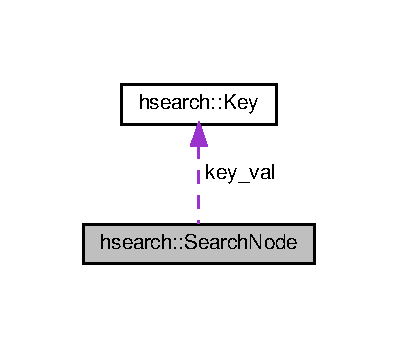
\includegraphics[width=191pt]{db/d43/structhsearch_1_1SearchNode__coll__graph}
\end{center}
\end{figure}
\subsection*{Public Member Functions}
\begin{DoxyCompactItemize}
\item 
\mbox{\Hypertarget{structhsearch_1_1SearchNode_a1e461dc25eef2e8de76dd7bd70042e22}\label{structhsearch_1_1SearchNode_a1e461dc25eef2e8de76dd7bd70042e22}} 
\hyperlink{structhsearch_1_1SearchNode_a1e461dc25eef2e8de76dd7bd70042e22}{Search\+Node} ()
\begin{DoxyCompactList}\small\item\em Default constructor. \end{DoxyCompactList}\item 
\hyperlink{structhsearch_1_1SearchNode_abc34e7eab1d4b3d269f9b360b77936a5}{Search\+Node} (const \hyperlink{structprm_1_1Node}{prm\+::\+Node} \&n)
\begin{DoxyCompactList}\small\item\em Create a new start node. \end{DoxyCompactList}\item 
void \hyperlink{structhsearch_1_1SearchNode_a0b8eea07c7013c327c70723182e43561}{Calc\+Key} (double km=0)
\begin{DoxyCompactList}\small\item\em Update the key values for a node. \end{DoxyCompactList}\item 
bool \hyperlink{structhsearch_1_1SearchNode_a936d6ea25917367b88adde4748c9143c}{operator$<$} (const \hyperlink{structhsearch_1_1SearchNode}{Search\+Node} \&rhs) const
\begin{DoxyCompactList}\small\item\em Custom function used for proper sorting of the open list by comparing the key values. \end{DoxyCompactList}\item 
bool \hyperlink{structhsearch_1_1SearchNode_a492955fe1a5cdfae1dc0474232cb7175}{operator$>$} (const \hyperlink{structhsearch_1_1SearchNode}{Search\+Node} \&rhs) const
\begin{DoxyCompactList}\small\item\em Custom function used for proper sorting of the open list by comparing the key values. \end{DoxyCompactList}\end{DoxyCompactItemize}
\subsection*{Public Attributes}
\begin{DoxyCompactItemize}
\item 
\mbox{\Hypertarget{structhsearch_1_1SearchNode_a891ec15f4f07e474fda39978a6ca6902}\label{structhsearch_1_1SearchNode_a891ec15f4f07e474fda39978a6ca6902}} 
std\+::shared\+\_\+ptr$<$ \hyperlink{structprm_1_1Node}{prm\+::\+Node} $>$ \hyperlink{structhsearch_1_1SearchNode_a891ec15f4f07e474fda39978a6ca6902}{node\+\_\+p} = nullptr
\begin{DoxyCompactList}\small\item\em contains info about ID, location and, neighbors \end{DoxyCompactList}\item 
\mbox{\Hypertarget{structhsearch_1_1SearchNode_ab0e32e34e1e2682c0cc7968df6dd7b85}\label{structhsearch_1_1SearchNode_ab0e32e34e1e2682c0cc7968df6dd7b85}} 
int \hyperlink{structhsearch_1_1SearchNode_ab0e32e34e1e2682c0cc7968df6dd7b85}{search\+\_\+id} = 0
\begin{DoxyCompactList}\small\item\em a unique id for the search node created \end{DoxyCompactList}\item 
\mbox{\Hypertarget{structhsearch_1_1SearchNode_a0f9510192452ac5efd6733eadfee38c2}\label{structhsearch_1_1SearchNode_a0f9510192452ac5efd6733eadfee38c2}} 
double \hyperlink{structhsearch_1_1SearchNode_a0f9510192452ac5efd6733eadfee38c2}{f\+\_\+val} = B\+I\+G\+\_\+\+N\+UM
\begin{DoxyCompactList}\small\item\em total node cost \end{DoxyCompactList}\item 
\mbox{\Hypertarget{structhsearch_1_1SearchNode_afc0b32b3c3c748e6585b76fc53553063}\label{structhsearch_1_1SearchNode_afc0b32b3c3c748e6585b76fc53553063}} 
double \hyperlink{structhsearch_1_1SearchNode_afc0b32b3c3c748e6585b76fc53553063}{g\+\_\+val} = B\+I\+G\+\_\+\+N\+UM
\begin{DoxyCompactList}\small\item\em path cost from start to this \end{DoxyCompactList}\item 
\mbox{\Hypertarget{structhsearch_1_1SearchNode_a8e25282237951762ced727eb0097abd9}\label{structhsearch_1_1SearchNode_a8e25282237951762ced727eb0097abd9}} 
double \hyperlink{structhsearch_1_1SearchNode_a8e25282237951762ced727eb0097abd9}{h\+\_\+val} = B\+I\+G\+\_\+\+N\+UM
\begin{DoxyCompactList}\small\item\em estimated cost from this to goal \end{DoxyCompactList}\item 
\mbox{\Hypertarget{structhsearch_1_1SearchNode_a85d37c5e72aa9fd323f68467f60c5eb0}\label{structhsearch_1_1SearchNode_a85d37c5e72aa9fd323f68467f60c5eb0}} 
double \hyperlink{structhsearch_1_1SearchNode_a85d37c5e72aa9fd323f68467f60c5eb0}{rhs\+\_\+val} = B\+I\+G\+\_\+\+N\+UM
\begin{DoxyCompactList}\small\item\em another estimate of the start distance used for incremental search methods \end{DoxyCompactList}\item 
\mbox{\Hypertarget{structhsearch_1_1SearchNode_adc5f4fb44ebe73e41ffdc6c5d22c526b}\label{structhsearch_1_1SearchNode_adc5f4fb44ebe73e41ffdc6c5d22c526b}} 
\hyperlink{structhsearch_1_1Key}{Key} \hyperlink{structhsearch_1_1SearchNode_adc5f4fb44ebe73e41ffdc6c5d22c526b}{key\+\_\+val}
\begin{DoxyCompactList}\small\item\em key values used to sort a \hyperlink{structhsearch_1_1SearchNode}{Search\+Node} in open list \end{DoxyCompactList}\item 
\mbox{\Hypertarget{structhsearch_1_1SearchNode_ad651df3e918ceb891c294945e9e41598}\label{structhsearch_1_1SearchNode_ad651df3e918ceb891c294945e9e41598}} 
std\+::shared\+\_\+ptr$<$ \hyperlink{structprm_1_1Node}{prm\+::\+Node} $>$ \hyperlink{structhsearch_1_1SearchNode_ad651df3e918ceb891c294945e9e41598}{parent\+\_\+p} = nullptr
\begin{DoxyCompactList}\small\item\em the parent of this node \end{DoxyCompactList}\item 
\mbox{\Hypertarget{structhsearch_1_1SearchNode_ae137174b53abd37ea386f3e3d9ebf462}\label{structhsearch_1_1SearchNode_ae137174b53abd37ea386f3e3d9ebf462}} 
status \hyperlink{structhsearch_1_1SearchNode_ae137174b53abd37ea386f3e3d9ebf462}{state} = New
\begin{DoxyCompactList}\small\item\em current status of the node \end{DoxyCompactList}\end{DoxyCompactItemize}


\subsection{Detailed Description}
Information used by a search algorithm. 

\subsection{Constructor \& Destructor Documentation}
\mbox{\Hypertarget{structhsearch_1_1SearchNode_abc34e7eab1d4b3d269f9b360b77936a5}\label{structhsearch_1_1SearchNode_abc34e7eab1d4b3d269f9b360b77936a5}} 
\index{hsearch\+::\+Search\+Node@{hsearch\+::\+Search\+Node}!Search\+Node@{Search\+Node}}
\index{Search\+Node@{Search\+Node}!hsearch\+::\+Search\+Node@{hsearch\+::\+Search\+Node}}
\subsubsection{\texorpdfstring{Search\+Node()}{SearchNode()}}
{\footnotesize\ttfamily hsearch\+::\+Search\+Node\+::\+Search\+Node (\begin{DoxyParamCaption}\item[{const \hyperlink{structprm_1_1Node}{prm\+::\+Node} \&}]{n }\end{DoxyParamCaption})}



Create a new start node. 


\begin{DoxyParams}{Parameters}
{\em n} & reference to a graph Node \\
\hline
\end{DoxyParams}


\subsection{Member Function Documentation}
\mbox{\Hypertarget{structhsearch_1_1SearchNode_a0b8eea07c7013c327c70723182e43561}\label{structhsearch_1_1SearchNode_a0b8eea07c7013c327c70723182e43561}} 
\index{hsearch\+::\+Search\+Node@{hsearch\+::\+Search\+Node}!Calc\+Key@{Calc\+Key}}
\index{Calc\+Key@{Calc\+Key}!hsearch\+::\+Search\+Node@{hsearch\+::\+Search\+Node}}
\subsubsection{\texorpdfstring{Calc\+Key()}{CalcKey()}}
{\footnotesize\ttfamily void hsearch\+::\+Search\+Node\+::\+Calc\+Key (\begin{DoxyParamCaption}\item[{double}]{km = {\ttfamily 0} }\end{DoxyParamCaption})}



Update the key values for a node. 


\begin{DoxyParams}{Parameters}
{\em km} & (optional) the key modifier used in an incremental D$\ast$ search, defaults to 0 \\
\hline
\end{DoxyParams}
\mbox{\Hypertarget{structhsearch_1_1SearchNode_a936d6ea25917367b88adde4748c9143c}\label{structhsearch_1_1SearchNode_a936d6ea25917367b88adde4748c9143c}} 
\index{hsearch\+::\+Search\+Node@{hsearch\+::\+Search\+Node}!operator$<$@{operator$<$}}
\index{operator$<$@{operator$<$}!hsearch\+::\+Search\+Node@{hsearch\+::\+Search\+Node}}
\subsubsection{\texorpdfstring{operator$<$()}{operator<()}}
{\footnotesize\ttfamily bool hsearch\+::\+Search\+Node\+::operator$<$ (\begin{DoxyParamCaption}\item[{const \hyperlink{structhsearch_1_1SearchNode}{Search\+Node} \&}]{rhs }\end{DoxyParamCaption}) const}



Custom function used for proper sorting of the open list by comparing the key values. 


\begin{DoxyParams}{Parameters}
{\em rhs} & another \hyperlink{structhsearch_1_1SearchNode}{Search\+Node} to compare against \\
\hline
\end{DoxyParams}
\begin{DoxyReturn}{Returns}
True if this node is less than rhs 
\end{DoxyReturn}
\mbox{\Hypertarget{structhsearch_1_1SearchNode_a492955fe1a5cdfae1dc0474232cb7175}\label{structhsearch_1_1SearchNode_a492955fe1a5cdfae1dc0474232cb7175}} 
\index{hsearch\+::\+Search\+Node@{hsearch\+::\+Search\+Node}!operator$>$@{operator$>$}}
\index{operator$>$@{operator$>$}!hsearch\+::\+Search\+Node@{hsearch\+::\+Search\+Node}}
\subsubsection{\texorpdfstring{operator$>$()}{operator>()}}
{\footnotesize\ttfamily bool hsearch\+::\+Search\+Node\+::operator$>$ (\begin{DoxyParamCaption}\item[{const \hyperlink{structhsearch_1_1SearchNode}{Search\+Node} \&}]{rhs }\end{DoxyParamCaption}) const}



Custom function used for proper sorting of the open list by comparing the key values. 


\begin{DoxyParams}{Parameters}
{\em rhs} & another \hyperlink{structhsearch_1_1SearchNode}{Search\+Node} to compare against \\
\hline
\end{DoxyParams}
\begin{DoxyReturn}{Returns}
True if this node is greater than rhs 
\end{DoxyReturn}


The documentation for this struct was generated from the following files\+:\begin{DoxyCompactItemize}
\item 
global\+\_\+search/include/global\+\_\+search/heuristic\+\_\+search.\+hpp\item 
global\+\_\+search/src/global\+\_\+search/heuristic\+\_\+search.\+cpp\end{DoxyCompactItemize}

\hypertarget{classhsearch_1_1ThetaStar}{}\section{hsearch\+:\+:Theta\+Star Class Reference}
\label{classhsearch_1_1ThetaStar}\index{hsearch\+::\+Theta\+Star@{hsearch\+::\+Theta\+Star}}


Theta$\ast$ any-\/angle path planner derived from the \hyperlink{classhsearch_1_1HSearch}{H\+Search} class.  




{\ttfamily \#include $<$heuristic\+\_\+search.\+hpp$>$}



Inheritance diagram for hsearch\+:\+:Theta\+Star\+:
\nopagebreak
\begin{figure}[H]
\begin{center}
\leavevmode
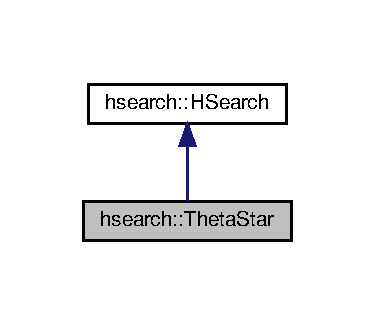
\includegraphics[width=180pt]{d9/db2/classhsearch_1_1ThetaStar__inherit__graph}
\end{center}
\end{figure}


Collaboration diagram for hsearch\+:\+:Theta\+Star\+:
\nopagebreak
\begin{figure}[H]
\begin{center}
\leavevmode
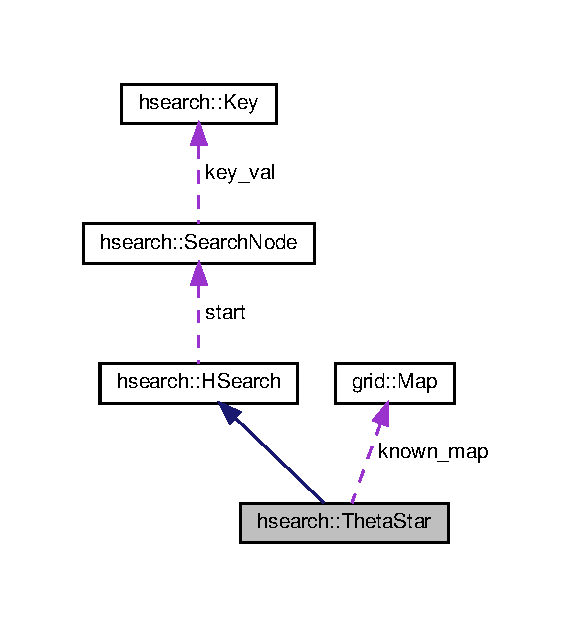
\includegraphics[width=275pt]{da/d4f/classhsearch_1_1ThetaStar__coll__graph}
\end{center}
\end{figure}
\subsection*{Public Member Functions}
\begin{DoxyCompactItemize}
\item 
\hyperlink{classhsearch_1_1ThetaStar_a9c3540ce3c1e93b8053eb97e62d71145}{Theta\+Star} (std\+::vector$<$ \hyperlink{structprm_1_1Node}{prm\+::\+Node} $>$ $\ast$node\+\_\+list, \hyperlink{structgrid_1_1Map}{grid\+::\+Map} map, double buffer)
\begin{DoxyCompactList}\small\item\em Constructor to initialize a Theta Star Search. \end{DoxyCompactList}\end{DoxyCompactItemize}
\subsection*{Protected Member Functions}
\begin{DoxyCompactItemize}
\item 
void \hyperlink{classhsearch_1_1ThetaStar_a852af6d668cbb3f58079125ba5740853}{Compute\+Cost} (\hyperlink{structhsearch_1_1SearchNode}{Search\+Node} \&s, \hyperlink{structhsearch_1_1SearchNode}{Search\+Node} \&sp)
\begin{DoxyCompactList}\small\item\em calculates the path 1 or path 2 cost between the two nodes \end{DoxyCompactList}\end{DoxyCompactItemize}
\subsection*{Protected Attributes}
\begin{DoxyCompactItemize}
\item 
\mbox{\Hypertarget{classhsearch_1_1ThetaStar_a90305133e71bfaa015747138383620da}\label{classhsearch_1_1ThetaStar_a90305133e71bfaa015747138383620da}} 
\hyperlink{structgrid_1_1Map}{grid\+::\+Map} \hyperlink{classhsearch_1_1ThetaStar_a90305133e71bfaa015747138383620da}{known\+\_\+map}
\begin{DoxyCompactList}\small\item\em Contains all known obstacles and the bounds of the map. \end{DoxyCompactList}\item 
\mbox{\Hypertarget{classhsearch_1_1ThetaStar_aba51580af01b2cdd040b94de00046271}\label{classhsearch_1_1ThetaStar_aba51580af01b2cdd040b94de00046271}} 
double \hyperlink{classhsearch_1_1ThetaStar_aba51580af01b2cdd040b94de00046271}{buffer\+\_\+radius}
\begin{DoxyCompactList}\small\item\em buffer radius when considering line of sight \end{DoxyCompactList}\end{DoxyCompactItemize}


\subsection{Detailed Description}
Theta$\ast$ any-\/angle path planner derived from the \hyperlink{classhsearch_1_1HSearch}{H\+Search} class. 

\subsection{Constructor \& Destructor Documentation}
\mbox{\Hypertarget{classhsearch_1_1ThetaStar_a9c3540ce3c1e93b8053eb97e62d71145}\label{classhsearch_1_1ThetaStar_a9c3540ce3c1e93b8053eb97e62d71145}} 
\index{hsearch\+::\+Theta\+Star@{hsearch\+::\+Theta\+Star}!Theta\+Star@{Theta\+Star}}
\index{Theta\+Star@{Theta\+Star}!hsearch\+::\+Theta\+Star@{hsearch\+::\+Theta\+Star}}
\subsubsection{\texorpdfstring{Theta\+Star()}{ThetaStar()}}
{\footnotesize\ttfamily hsearch\+::\+Theta\+Star\+::\+Theta\+Star (\begin{DoxyParamCaption}\item[{std\+::vector$<$ \hyperlink{structprm_1_1Node}{prm\+::\+Node} $>$ $\ast$}]{node\+\_\+list,  }\item[{\hyperlink{structgrid_1_1Map}{grid\+::\+Map}}]{map,  }\item[{double}]{buffer }\end{DoxyParamCaption})}



Constructor to initialize a Theta Star Search. 


\begin{DoxyParams}{Parameters}
{\em node\+\_\+list} & pointer to a vector of Nodes that create a graph \\
\hline
{\em map} & a known the map used to create the graph \\
\hline
{\em buffer} & a buffer radius to account for in line of sight checks \\
\hline
\end{DoxyParams}


\subsection{Member Function Documentation}
\mbox{\Hypertarget{classhsearch_1_1ThetaStar_a852af6d668cbb3f58079125ba5740853}\label{classhsearch_1_1ThetaStar_a852af6d668cbb3f58079125ba5740853}} 
\index{hsearch\+::\+Theta\+Star@{hsearch\+::\+Theta\+Star}!Compute\+Cost@{Compute\+Cost}}
\index{Compute\+Cost@{Compute\+Cost}!hsearch\+::\+Theta\+Star@{hsearch\+::\+Theta\+Star}}
\subsubsection{\texorpdfstring{Compute\+Cost()}{ComputeCost()}}
{\footnotesize\ttfamily void hsearch\+::\+Theta\+Star\+::\+Compute\+Cost (\begin{DoxyParamCaption}\item[{\hyperlink{structhsearch_1_1SearchNode}{Search\+Node} \&}]{s,  }\item[{\hyperlink{structhsearch_1_1SearchNode}{Search\+Node} \&}]{sp }\end{DoxyParamCaption})\hspace{0.3cm}{\ttfamily [protected]}, {\ttfamily [virtual]}}



calculates the path 1 or path 2 cost between the two nodes 


\begin{DoxyParams}{Parameters}
{\em s} & the current node being expanded \\
\hline
{\em sp} & the neighbor node being evaluated \\
\hline
\end{DoxyParams}


Implements \hyperlink{classhsearch_1_1HSearch_a5d325955c4faedaca0c68155fd1f7e69}{hsearch\+::\+H\+Search}.



The documentation for this class was generated from the following files\+:\begin{DoxyCompactItemize}
\item 
global\+\_\+search/include/global\+\_\+search/\hyperlink{heuristic__search_8hpp}{heuristic\+\_\+search.\+hpp}\item 
global\+\_\+search/src/global\+\_\+search/\hyperlink{heuristic__search_8cpp}{heuristic\+\_\+search.\+cpp}\end{DoxyCompactItemize}

\chapter{File Documentation}
\hypertarget{heuristic__search_8hpp}{}\section{global\+\_\+search/include/global\+\_\+search/heuristic\+\_\+search.hpp File Reference}
\label{heuristic__search_8hpp}\index{global\+\_\+search/include/global\+\_\+search/heuristic\+\_\+search.\+hpp@{global\+\_\+search/include/global\+\_\+search/heuristic\+\_\+search.\+hpp}}


A library containing classes to perform various types of search algorithms.  


{\ttfamily \#include $<$memory$>$}\newline
{\ttfamily \#include $<$cmath$>$}\newline
{\ttfamily \#include \char`\"{}rigid2d/rigid2d.\+hpp\char`\"{}}\newline
{\ttfamily \#include \char`\"{}roadmap/prm.\+hpp\char`\"{}}\newline
{\ttfamily \#include \char`\"{}roadmap/grid.\+hpp\char`\"{}}\newline
Include dependency graph for heuristic\+\_\+search.\+hpp\+:\nopagebreak
\begin{figure}[H]
\begin{center}
\leavevmode
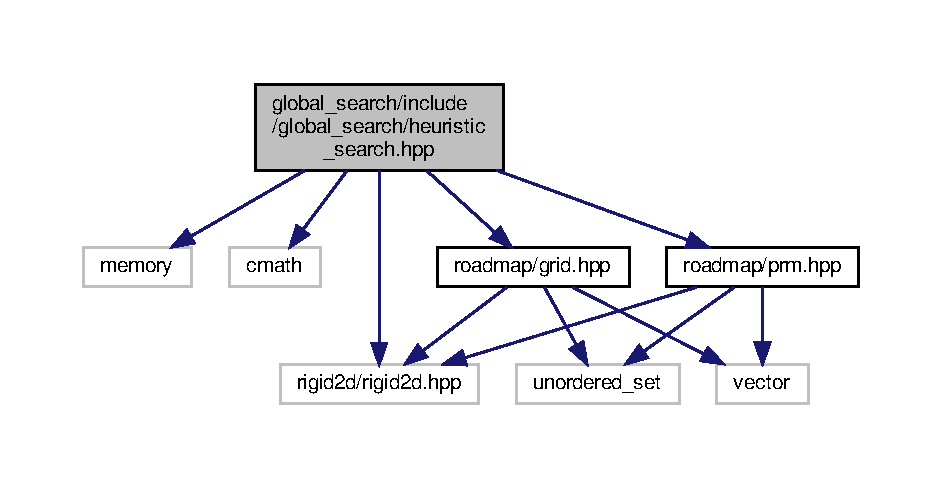
\includegraphics[width=350pt]{d2/d80/heuristic__search_8hpp__incl}
\end{center}
\end{figure}
This graph shows which files directly or indirectly include this file\+:\nopagebreak
\begin{figure}[H]
\begin{center}
\leavevmode
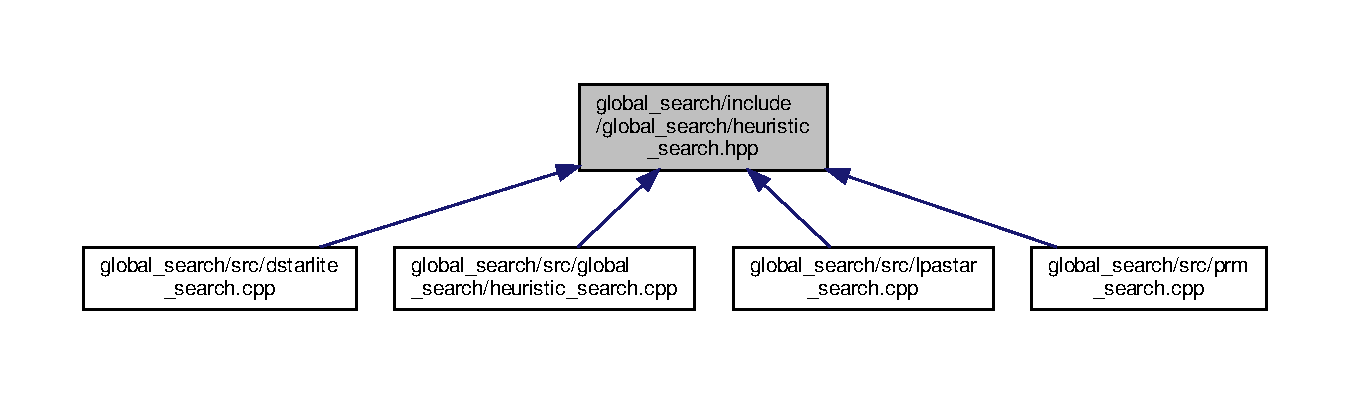
\includegraphics[width=350pt]{d0/d88/heuristic__search_8hpp__dep__incl}
\end{center}
\end{figure}
\subsection*{Classes}
\begin{DoxyCompactItemize}
\item 
struct \hyperlink{structhsearch_1_1SearchNode}{hsearch\+::\+Search\+Node}
\begin{DoxyCompactList}\small\item\em Information used by a search algorithm. \end{DoxyCompactList}\item 
class \hyperlink{classhsearch_1_1HSearch}{hsearch\+::\+H\+Search}
\begin{DoxyCompactList}\small\item\em The base class to define a heuristic based search algorithm. This class has no Compute\+Cost funtion which is required to find the shortest path. This function is defined in the derived class to determine the type of search. Some searched also have a different flow for finding the shortest path, which is why the Compute\+Shortest\+Path method is virtual. \end{DoxyCompactList}\item 
class \hyperlink{classhsearch_1_1AStar}{hsearch\+::\+A\+Star}
\begin{DoxyCompactList}\small\item\em A$\ast$ Search class derived from the \hyperlink{classhsearch_1_1HSearch}{H\+Search} class. \end{DoxyCompactList}\item 
class \hyperlink{classhsearch_1_1ThetaStar}{hsearch\+::\+Theta\+Star}
\begin{DoxyCompactList}\small\item\em Theta$\ast$ any-\/angle path planner derived from the \hyperlink{classhsearch_1_1HSearch}{H\+Search} class. \end{DoxyCompactList}\end{DoxyCompactItemize}
\subsection*{Enumerations}
\begin{DoxyCompactItemize}
\item 
\mbox{\Hypertarget{heuristic__search_8hpp_a544e6b02038f7495f0ef622404fdfd79}\label{heuristic__search_8hpp_a544e6b02038f7495f0ef622404fdfd79}} 
enum \hyperlink{heuristic__search_8hpp_a544e6b02038f7495f0ef622404fdfd79}{hsearch\+::status} \{ {\bfseries New}, 
{\bfseries Open}, 
{\bfseries Closed}
 \}\begin{DoxyCompactList}\small\item\em Used to track if a node is New, on the open, or on the closed list. \end{DoxyCompactList}
\end{DoxyCompactItemize}
\subsection*{Functions}
\begin{DoxyCompactItemize}
\item 
std\+::ostream \& \hyperlink{heuristic__search_8hpp_a18e6565e8bc131f1b0121fe1c3d70f90}{hsearch\+::operator$<$$<$} (std\+::ostream \&os, const Search\+Node \&n)
\begin{DoxyCompactList}\small\item\em Overload the cout operator to print the info in a \hyperlink{structhsearch_1_1SearchNode}{Search\+Node}. \end{DoxyCompactList}\end{DoxyCompactItemize}


\subsection{Detailed Description}
A library containing classes to perform various types of search algorithms. 



\subsection{Function Documentation}
\mbox{\Hypertarget{heuristic__search_8hpp_file_a18e6565e8bc131f1b0121fe1c3d70f90}\label{heuristic__search_8hpp_file_a18e6565e8bc131f1b0121fe1c3d70f90}} 
\index{heuristic\+\_\+search.\+hpp@{heuristic\+\_\+search.\+hpp}!operator$<$$<$@{operator$<$$<$}}
\index{operator$<$$<$@{operator$<$$<$}!heuristic\+\_\+search.\+hpp@{heuristic\+\_\+search.\+hpp}}
\subsubsection{\texorpdfstring{operator$<$$<$()}{operator<<()}}
{\footnotesize\ttfamily std\+::ostream \& hsearch\+::operator$<$$<$ (\begin{DoxyParamCaption}\item[{std\+::ostream \&}]{os,  }\item[{const \hyperlink{structhsearch_1_1SearchNode}{Search\+Node} \&}]{n }\end{DoxyParamCaption})}



Overload the cout operator to print the info in a Search\+Node. 


\begin{DoxyParams}{Parameters}
{\em os} & the output stream \\
\hline
{\em n} & a Search\+Node reference \\
\hline
\end{DoxyParams}
\begin{DoxyReturn}{Returns}
an output stream 
\end{DoxyReturn}

\hypertarget{potential__fields_8hpp}{}\section{global\+\_\+search/include/global\+\_\+search/potential\+\_\+fields.hpp File Reference}
\label{potential__fields_8hpp}\index{global\+\_\+search/include/global\+\_\+search/potential\+\_\+fields.\+hpp@{global\+\_\+search/include/global\+\_\+search/potential\+\_\+fields.\+hpp}}


A library to plan based on a potential field.  


{\ttfamily \#include \char`\"{}rigid2d/rigid2d.\+hpp\char`\"{}}\newline
{\ttfamily \#include \char`\"{}roadmap/grid.\+hpp\char`\"{}}\newline
Include dependency graph for potential\+\_\+fields.\+hpp\+:\nopagebreak
\begin{figure}[H]
\begin{center}
\leavevmode
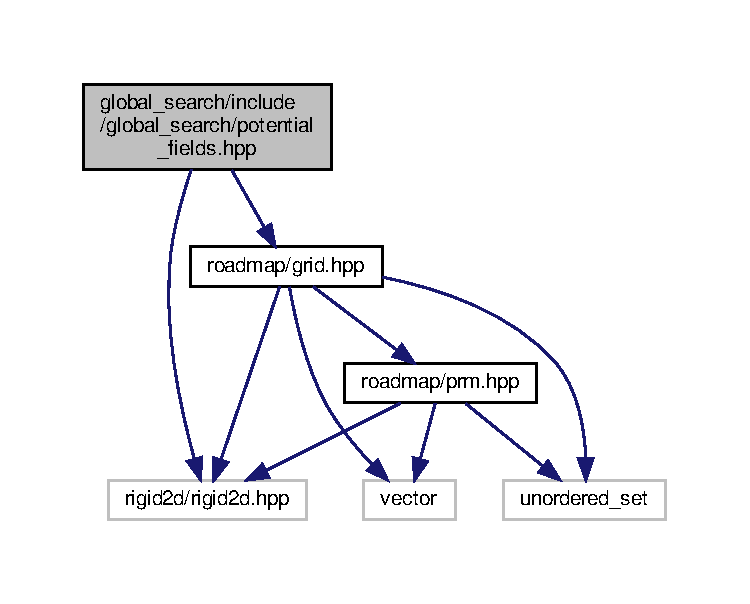
\includegraphics[width=350pt]{de/ddb/potential__fields_8hpp__incl}
\end{center}
\end{figure}
This graph shows which files directly or indirectly include this file\+:\nopagebreak
\begin{figure}[H]
\begin{center}
\leavevmode
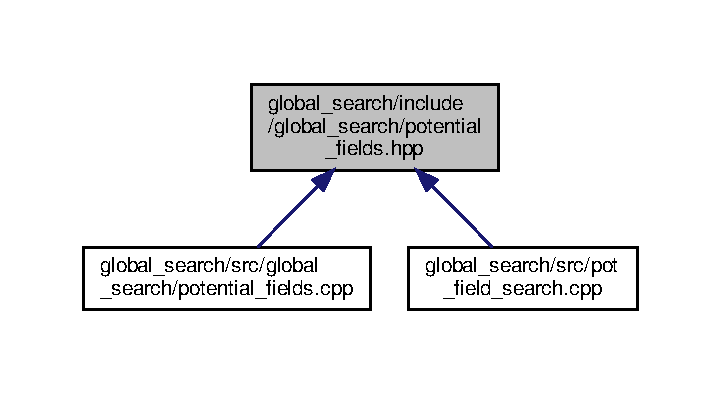
\includegraphics[width=346pt]{d8/dd0/potential__fields_8hpp__dep__incl}
\end{center}
\end{figure}
\subsection*{Classes}
\begin{DoxyCompactItemize}
\item 
class \hyperlink{classpfield_1_1PtField}{pfield\+::\+Pt\+Field}
\begin{DoxyCompactList}\small\item\em brief class to allow planning \end{DoxyCompactList}\end{DoxyCompactItemize}
\subsection*{Macros}
\begin{DoxyCompactItemize}
\item 
\mbox{\Hypertarget{potential__fields_8hpp_a44b8ad40964aabfb40ae3a0625190475}\label{potential__fields_8hpp_a44b8ad40964aabfb40ae3a0625190475}} 
\#define \hyperlink{potential__fields_8hpp_a44b8ad40964aabfb40ae3a0625190475}{B\+I\+G\+\_\+\+N\+UM}~10000.\+0
\begin{DoxyCompactList}\small\item\em A number used to represent a large cost. \end{DoxyCompactList}\end{DoxyCompactItemize}


\subsection{Detailed Description}
A library to plan based on a potential field. 


\hypertarget{dstarlite__search_8cpp}{}\section{global\+\_\+search/src/dstarlite\+\_\+search.cpp File Reference}
\label{dstarlite__search_8cpp}\index{global\+\_\+search/src/dstarlite\+\_\+search.\+cpp@{global\+\_\+search/src/dstarlite\+\_\+search.\+cpp}}


Node to create, draw, and plan on a changing grid map.  


{\ttfamily \#include $<$vector$>$}\newline
{\ttfamily \#include $<$algorithm$>$}\newline
{\ttfamily \#include $<$Xml\+Rpc\+Value.\+h$>$}\newline
{\ttfamily \#include $<$ros/ros.\+h$>$}\newline
{\ttfamily \#include \char`\"{}geometry\+\_\+msgs/\+Point.\+h\char`\"{}}\newline
{\ttfamily \#include \char`\"{}visualization\+\_\+msgs/\+Marker\+Array.\+h\char`\"{}}\newline
{\ttfamily \#include \char`\"{}visualization\+\_\+msgs/\+Marker.\+h\char`\"{}}\newline
{\ttfamily \#include \char`\"{}global\+\_\+search/heuristic\+\_\+search.\+hpp\char`\"{}}\newline
{\ttfamily \#include \char`\"{}rigid2d/rigid2d.\+hpp\char`\"{}}\newline
{\ttfamily \#include \char`\"{}roadmap/prm.\+hpp\char`\"{}}\newline
{\ttfamily \#include \char`\"{}roadmap/utility.\+hpp\char`\"{}}\newline
Include dependency graph for dstarlite\+\_\+search.\+cpp\+:\nopagebreak
\begin{figure}[H]
\begin{center}
\leavevmode
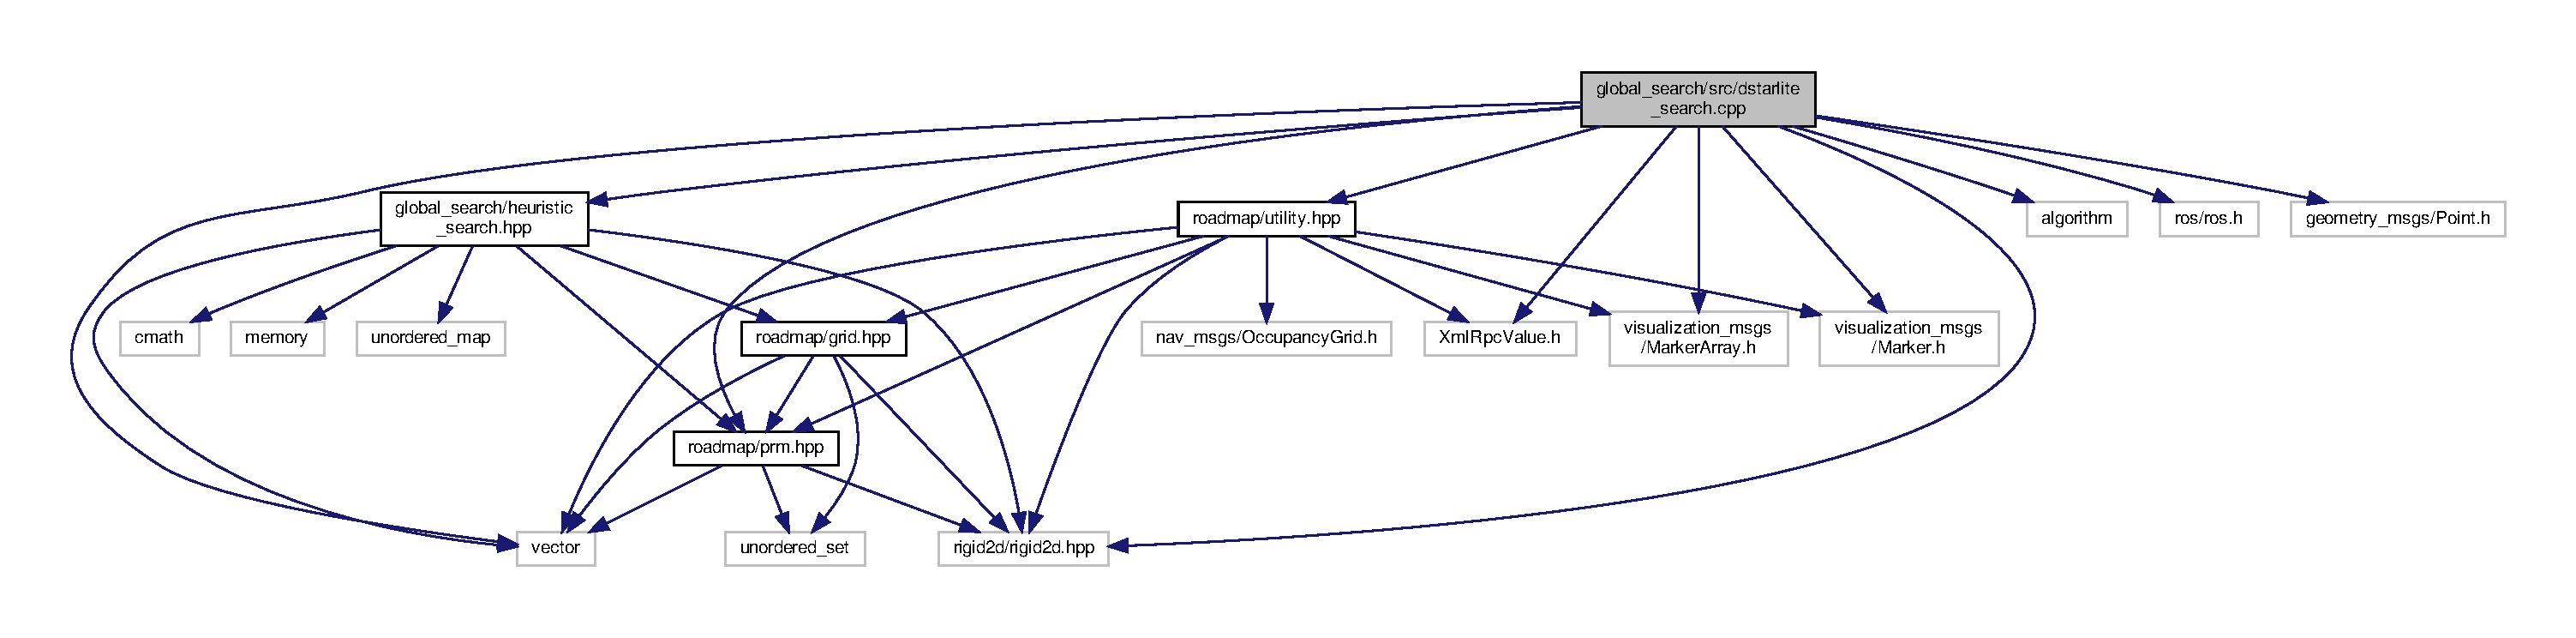
\includegraphics[width=350pt]{dd/d81/dstarlite__search_8cpp__incl}
\end{center}
\end{figure}
\subsection*{Functions}
\begin{DoxyCompactItemize}
\item 
\mbox{\Hypertarget{dstarlite__search_8cpp_a3c04138a5bfe5d72780bb7e82a18e627}\label{dstarlite__search_8cpp_a3c04138a5bfe5d72780bb7e82a18e627}} 
int {\bfseries main} (int argc, char $\ast$$\ast$argv)
\end{DoxyCompactItemize}


\subsection{Detailed Description}
Node to create, draw, and plan on a changing grid map. 

P\+A\+R\+A\+M\+E\+T\+E\+RS\+: obstacles (std\+::vector$<$std\+::vector$<$std\+::vector$<$double$>$) a vector of polygons represented by a vector of x,y coords for the verticies map\+\_\+x\+\_\+lims (std\+::vector$<$double$>$) \mbox{[}xmin, xmax\mbox{]} of the map map\+\_\+y\+\_\+lims (std\+::vector$<$double$>$) \mbox{[}ymin, ymax\mbox{]} of the map robot\+\_\+radius (double) buffer radius to avoid collisions with the robot body cell\+\_\+size (double) scaling factor for the map grid\+\_\+res (double) scaling factor for the grid cell size r (std\+::vector$<$int$>$) color values g (std\+::vector$<$int$>$) color values b (std\+::vector$<$int$>$) color values start std\+::vector$<$double$>$ two double values representing the x,y of the start point goal std\+::vector$<$double$>$ two double values representing the x,y of the goal point sensor\+\_\+range (double) double value representing the range of a simulated sensor fixed to the center of the robot P\+U\+B\+L\+I\+S\+H\+ES\+: /visualization\+\_\+marker\+\_\+array (visualization\+\_\+msgs\+::\+Marker\+Array) markers /grid\+\_\+map (nav\+\_\+msgs\+::\+Occupancy\+Grid) occupancy data 
\hypertarget{heuristic__search_8cpp}{}\section{global\+\_\+search/src/global\+\_\+search/heuristic\+\_\+search.cpp File Reference}
\label{heuristic__search_8cpp}\index{global\+\_\+search/src/global\+\_\+search/heuristic\+\_\+search.\+cpp@{global\+\_\+search/src/global\+\_\+search/heuristic\+\_\+search.\+cpp}}


A library containing classes to perform various types of search algorithms.  


{\ttfamily \#include $<$algorithm$>$}\newline
{\ttfamily \#include $<$cmath$>$}\newline
{\ttfamily \#include $<$iostream$>$}\newline
{\ttfamily \#include $<$memory$>$}\newline
{\ttfamily \#include \char`\"{}global\+\_\+search/heuristic\+\_\+search.\+hpp\char`\"{}}\newline
{\ttfamily \#include \char`\"{}rigid2d/rigid2d.\+hpp\char`\"{}}\newline
{\ttfamily \#include \char`\"{}roadmap/collision.\+hpp\char`\"{}}\newline
{\ttfamily \#include \char`\"{}roadmap/prm.\+hpp\char`\"{}}\newline
{\ttfamily \#include \char`\"{}roadmap/grid.\+hpp\char`\"{}}\newline
Include dependency graph for heuristic\+\_\+search.\+cpp\+:\nopagebreak
\begin{figure}[H]
\begin{center}
\leavevmode
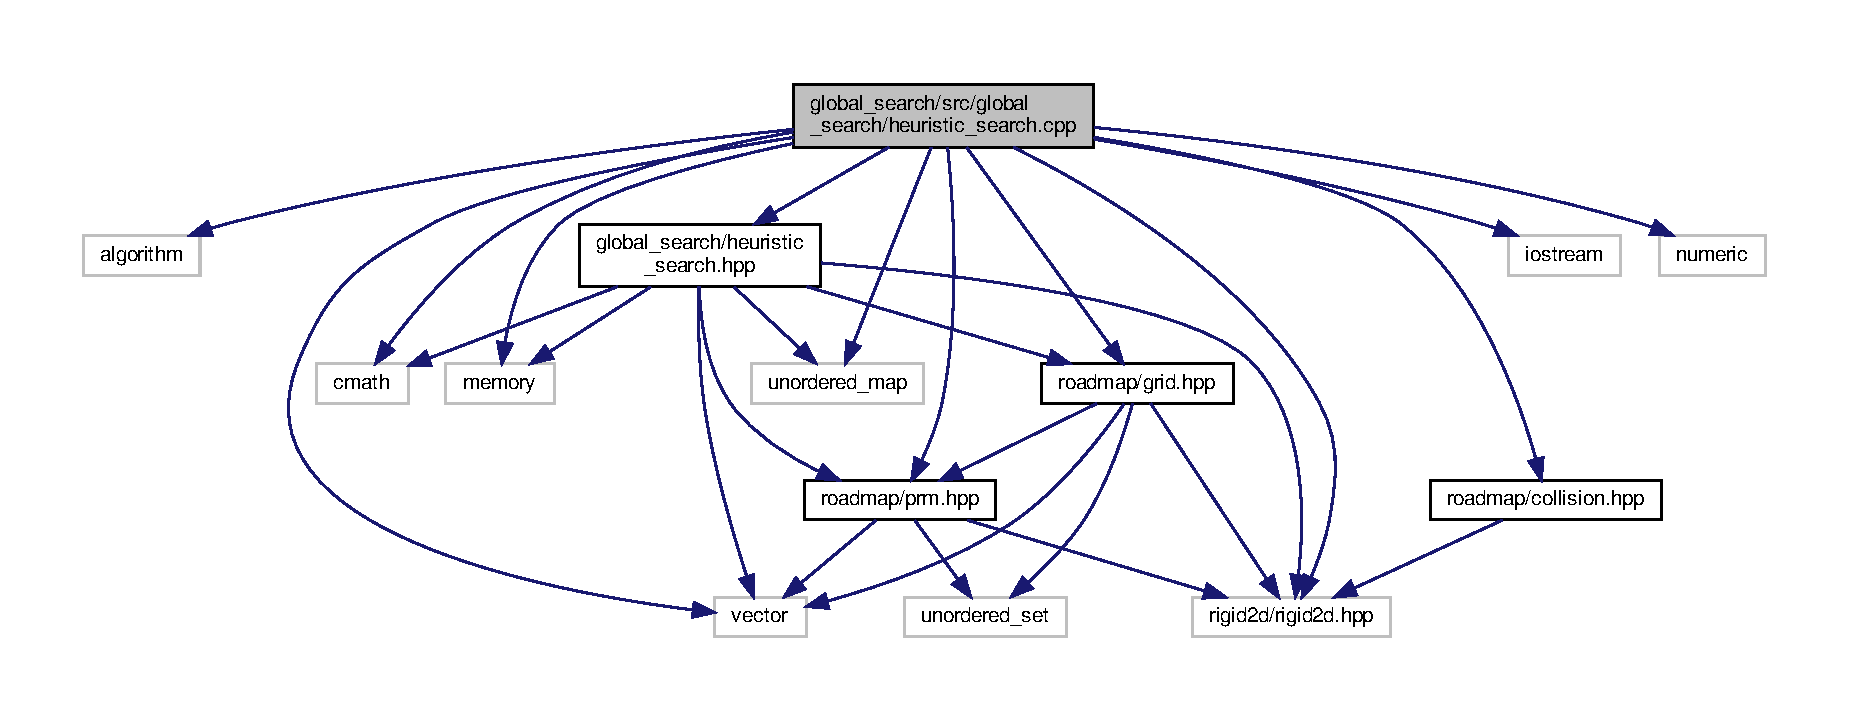
\includegraphics[width=350pt]{dd/d48/heuristic__search_8cpp__incl}
\end{center}
\end{figure}
\subsection*{Functions}
\begin{DoxyCompactItemize}
\item 
std\+::ostream \& \hyperlink{heuristic__search_8hpp_a18e6565e8bc131f1b0121fe1c3d70f90}{hsearch\+::operator$<$$<$} (std\+::ostream \&os, const Search\+Node \&n)
\begin{DoxyCompactList}\small\item\em Overload the cout operator to print the info in a \hyperlink{structhsearch_1_1SearchNode}{Search\+Node}. \end{DoxyCompactList}\end{DoxyCompactItemize}


\subsection{Detailed Description}
A library containing classes to perform various types of search algorithms. 



\subsection{Function Documentation}
\mbox{\Hypertarget{heuristic__search_8hpp_file_a18e6565e8bc131f1b0121fe1c3d70f90}\label{heuristic__search_8hpp_file_a18e6565e8bc131f1b0121fe1c3d70f90}} 
\index{heuristic\+\_\+search.\+cpp@{heuristic\+\_\+search.\+cpp}!operator$<$$<$@{operator$<$$<$}}
\index{operator$<$$<$@{operator$<$$<$}!heuristic\+\_\+search.\+cpp@{heuristic\+\_\+search.\+cpp}}
\subsubsection{\texorpdfstring{operator$<$$<$()}{operator<<()}}
{\footnotesize\ttfamily std\+::ostream \& hsearch\+::operator$<$$<$ (\begin{DoxyParamCaption}\item[{std\+::ostream \&}]{os,  }\item[{const \hyperlink{structhsearch_1_1SearchNode}{Search\+Node} \&}]{n }\end{DoxyParamCaption})}



Overload the cout operator to print the info in a Search\+Node. 


\begin{DoxyParams}{Parameters}
{\em os} & the output stream \\
\hline
{\em n} & a Search\+Node reference \\
\hline
\end{DoxyParams}
\begin{DoxyReturn}{Returns}
an output stream 
\end{DoxyReturn}

\hypertarget{potential__fields_8cpp}{}\section{global\+\_\+search/src/global\+\_\+search/potential\+\_\+fields.cpp File Reference}
\label{potential__fields_8cpp}\index{global\+\_\+search/src/global\+\_\+search/potential\+\_\+fields.\+cpp@{global\+\_\+search/src/global\+\_\+search/potential\+\_\+fields.\+cpp}}


A library to plan based on a potential field.  


{\ttfamily \#include $<$vector$>$}\newline
{\ttfamily \#include \char`\"{}global\+\_\+search/potential\+\_\+fields.\+hpp\char`\"{}}\newline
{\ttfamily \#include \char`\"{}rigid2d/rigid2d.\+hpp\char`\"{}}\newline
{\ttfamily \#include \char`\"{}roadmap/collision.\+hpp\char`\"{}}\newline
{\ttfamily \#include \char`\"{}roadmap/grid.\+hpp\char`\"{}}\newline
Include dependency graph for potential\+\_\+fields.\+cpp\+:\nopagebreak
\begin{figure}[H]
\begin{center}
\leavevmode
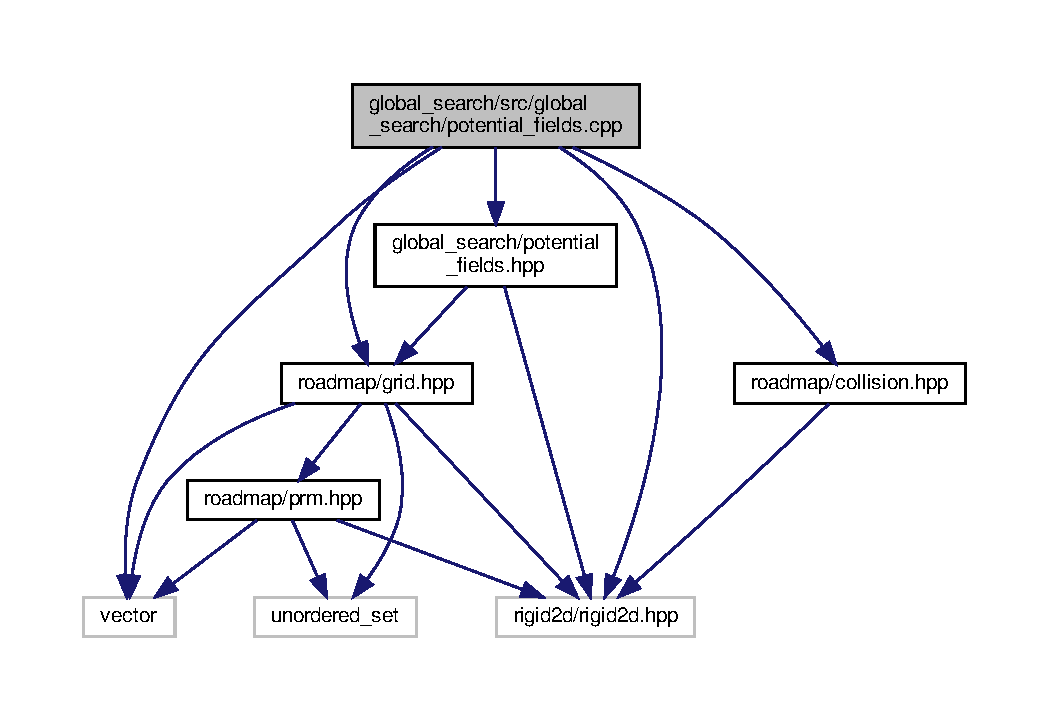
\includegraphics[width=350pt]{de/d81/potential__fields_8cpp__incl}
\end{center}
\end{figure}


\subsection{Detailed Description}
A library to plan based on a potential field. 


\hypertarget{lpastar__search_8cpp}{}\section{global\+\_\+search/src/lpastar\+\_\+search.cpp File Reference}
\label{lpastar__search_8cpp}\index{global\+\_\+search/src/lpastar\+\_\+search.\+cpp@{global\+\_\+search/src/lpastar\+\_\+search.\+cpp}}


Node to create, draw, and plan on a changing grid map.  


{\ttfamily \#include $<$vector$>$}\newline
{\ttfamily \#include $<$algorithm$>$}\newline
{\ttfamily \#include $<$Xml\+Rpc\+Value.\+h$>$}\newline
{\ttfamily \#include $<$ros/ros.\+h$>$}\newline
{\ttfamily \#include \char`\"{}geometry\+\_\+msgs/\+Point.\+h\char`\"{}}\newline
{\ttfamily \#include \char`\"{}visualization\+\_\+msgs/\+Marker\+Array.\+h\char`\"{}}\newline
{\ttfamily \#include \char`\"{}visualization\+\_\+msgs/\+Marker.\+h\char`\"{}}\newline
{\ttfamily \#include \char`\"{}global\+\_\+search/heuristic\+\_\+search.\+hpp\char`\"{}}\newline
{\ttfamily \#include \char`\"{}rigid2d/rigid2d.\+hpp\char`\"{}}\newline
{\ttfamily \#include \char`\"{}roadmap/prm.\+hpp\char`\"{}}\newline
{\ttfamily \#include \char`\"{}roadmap/utility.\+hpp\char`\"{}}\newline
Include dependency graph for lpastar\+\_\+search.\+cpp\+:\nopagebreak
\begin{figure}[H]
\begin{center}
\leavevmode
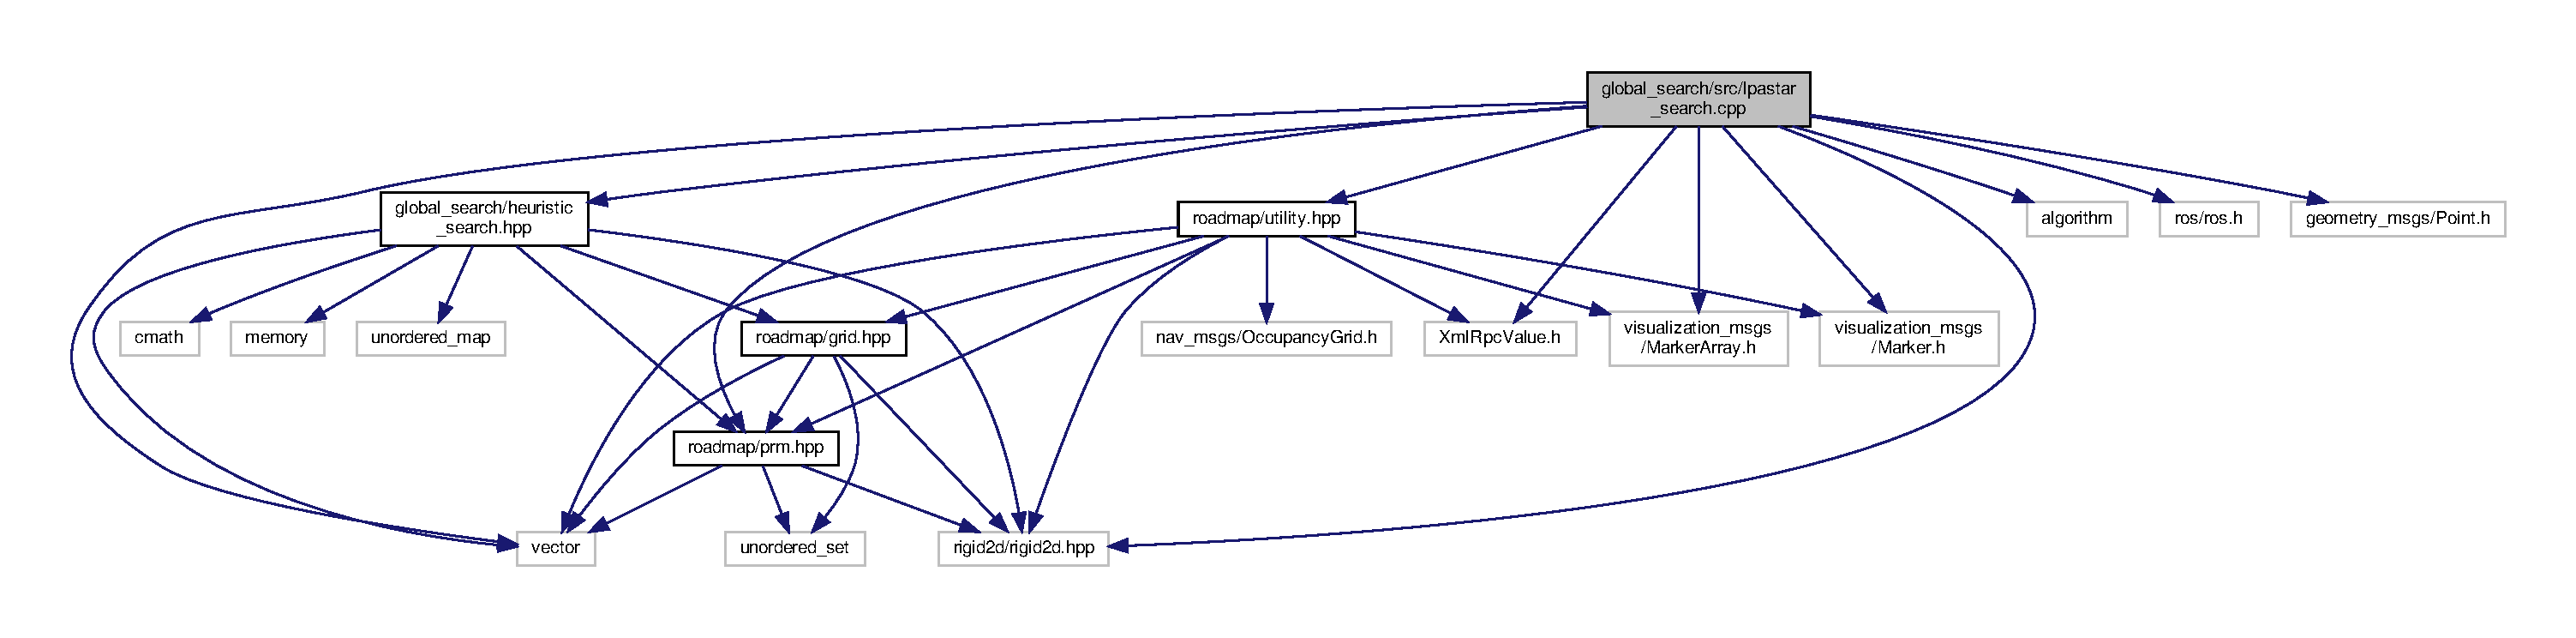
\includegraphics[width=350pt]{dc/dd7/lpastar__search_8cpp__incl}
\end{center}
\end{figure}
\subsection*{Functions}
\begin{DoxyCompactItemize}
\item 
\mbox{\Hypertarget{lpastar__search_8cpp_a3c04138a5bfe5d72780bb7e82a18e627}\label{lpastar__search_8cpp_a3c04138a5bfe5d72780bb7e82a18e627}} 
int {\bfseries main} (int argc, char $\ast$$\ast$argv)
\end{DoxyCompactItemize}


\subsection{Detailed Description}
Node to create, draw, and plan on a changing grid map. 

P\+A\+R\+A\+M\+E\+T\+E\+RS\+: obstacles (std\+::vector$<$std\+::vector$<$std\+::vector$<$double$>$) a vector of polygons represented by a vector of x,y coords for the verticies map\+\_\+x\+\_\+lims (std\+::vector$<$double$>$) \mbox{[}xmin, xmax\mbox{]} of the map map\+\_\+y\+\_\+lims (std\+::vector$<$double$>$) \mbox{[}ymin, ymax\mbox{]} of the map robot\+\_\+radius (double) buffer radius to avoid collisions with the robot body cell\+\_\+size (double) scaling factor for the map grid\+\_\+res (double) scaling factor for the grid cell size r (std\+::vector$<$int$>$) color values g (std\+::vector$<$int$>$) color values b (std\+::vector$<$int$>$) color values start std\+::vector$<$double$>$ two double values representing the x,y of the start point goal std\+::vector$<$double$>$ two double values representing the x,y of the goal point P\+U\+B\+L\+I\+S\+H\+ES\+: /visualization\+\_\+marker\+\_\+array (visualization\+\_\+msgs\+::\+Marker\+Array) markers /grid\+\_\+map (nav\+\_\+msgs\+::\+Occupancy\+Grid) occupancy data 
\hypertarget{pot__field__search_8cpp}{}\section{global\+\_\+search/src/pot\+\_\+field\+\_\+search.cpp File Reference}
\label{pot__field__search_8cpp}\index{global\+\_\+search/src/pot\+\_\+field\+\_\+search.\+cpp@{global\+\_\+search/src/pot\+\_\+field\+\_\+search.\+cpp}}


Node to plan on the map using potential fields.  


{\ttfamily \#include $<$vector$>$}\newline
{\ttfamily \#include $<$algorithm$>$}\newline
{\ttfamily \#include $<$Xml\+Rpc\+Value.\+h$>$}\newline
{\ttfamily \#include $<$ros/ros.\+h$>$}\newline
{\ttfamily \#include \char`\"{}geometry\+\_\+msgs/\+Point.\+h\char`\"{}}\newline
{\ttfamily \#include \char`\"{}visualization\+\_\+msgs/\+Marker\+Array.\+h\char`\"{}}\newline
{\ttfamily \#include \char`\"{}visualization\+\_\+msgs/\+Marker.\+h\char`\"{}}\newline
{\ttfamily \#include \char`\"{}global\+\_\+search/potential\+\_\+fields.\+hpp\char`\"{}}\newline
{\ttfamily \#include \char`\"{}rigid2d/rigid2d.\+hpp\char`\"{}}\newline
{\ttfamily \#include \char`\"{}roadmap/prm.\+hpp\char`\"{}}\newline
{\ttfamily \#include \char`\"{}roadmap/utility.\+hpp\char`\"{}}\newline
Include dependency graph for pot\+\_\+field\+\_\+search.\+cpp\+:\nopagebreak
\begin{figure}[H]
\begin{center}
\leavevmode
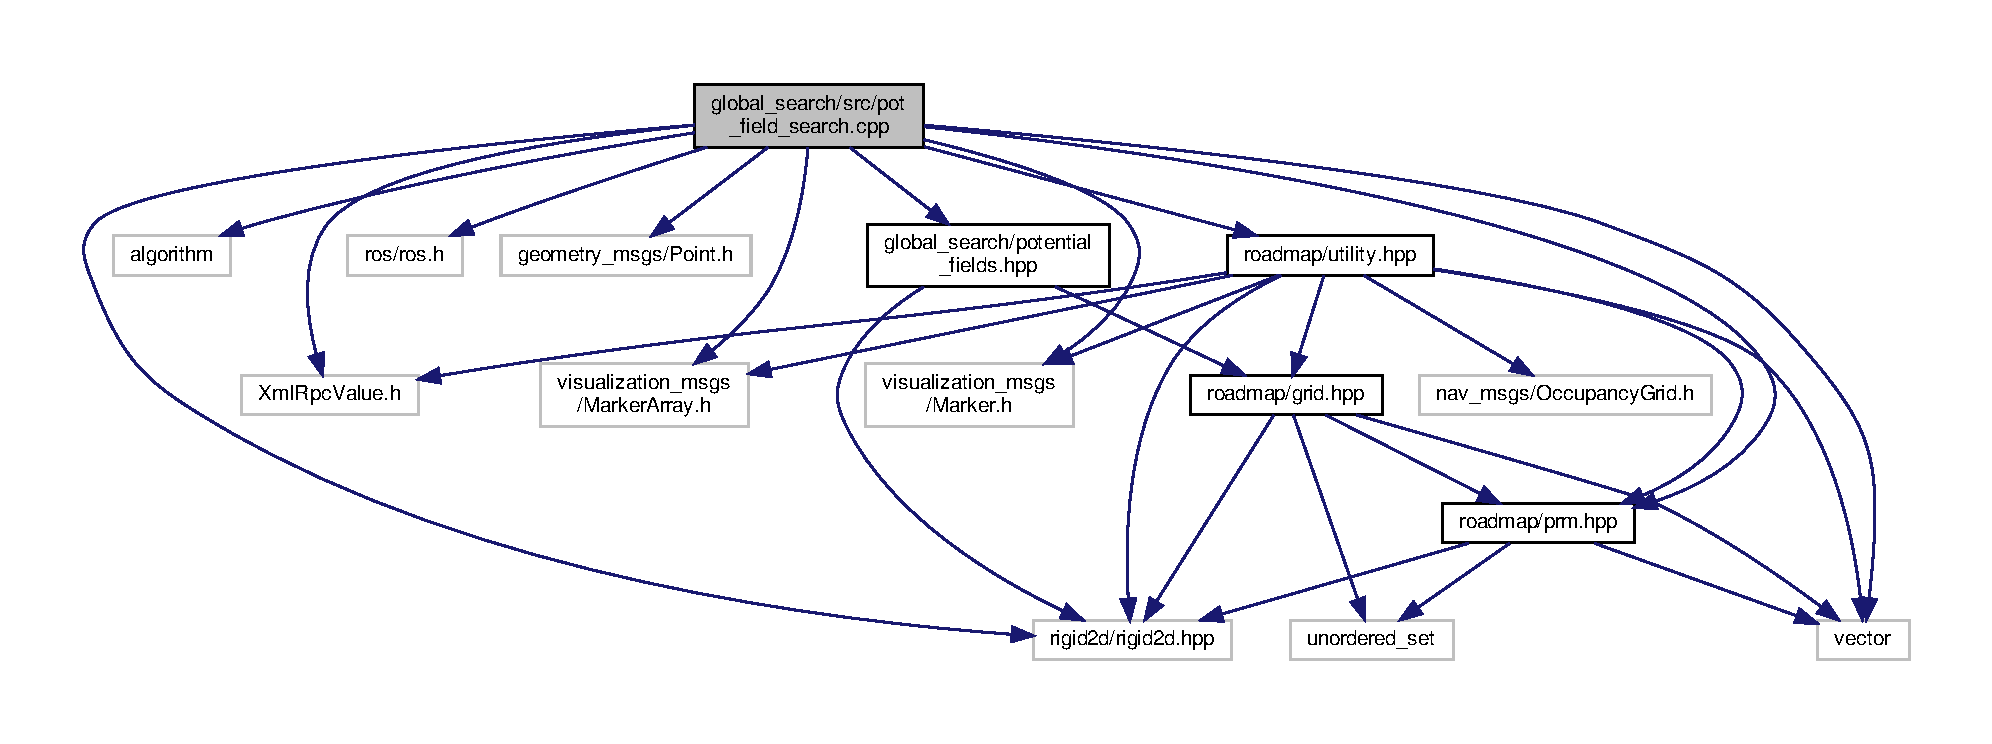
\includegraphics[width=350pt]{dc/dc7/pot__field__search_8cpp__incl}
\end{center}
\end{figure}
\subsection*{Functions}
\begin{DoxyCompactItemize}
\item 
\mbox{\Hypertarget{pot__field__search_8cpp_a3c04138a5bfe5d72780bb7e82a18e627}\label{pot__field__search_8cpp_a3c04138a5bfe5d72780bb7e82a18e627}} 
int {\bfseries main} (int argc, char $\ast$$\ast$argv)
\end{DoxyCompactItemize}


\subsection{Detailed Description}
Node to plan on the map using potential fields. 

P\+A\+R\+A\+M\+E\+T\+E\+RS\+: obstacles (std\+::vector$<$std\+::vector$<$std\+::vector$<$double$>$) a vector of polygons represented by a vector of x,y coords for the verticies map\+\_\+x\+\_\+lims (std\+::vector$<$double$>$) \mbox{[}xmin, xmax\mbox{]} of the map map\+\_\+y\+\_\+lims (std\+::vector$<$double$>$) \mbox{[}ymin, ymax\mbox{]} of the map robot\+\_\+radius (double) buffer radius to avoid collisions with the robot body cell\+\_\+size (double) distance of each cell r (std\+::vector$<$int$>$) color values g (std\+::vector$<$int$>$) color values b (std\+::vector$<$int$>$) color values start std\+::vector$<$double$>$ two double values representing the x,y of the start point goal std\+::vector$<$double$>$ two double values representing the x,y of the goal point P\+U\+B\+L\+I\+S\+H\+ES\+: /visualization\+\_\+marker\+\_\+array (visualization\+\_\+msgs\+::\+Marker\+Array) markers 
\hypertarget{prm__search_8cpp}{}\section{global\+\_\+search/src/prm\+\_\+search.cpp File Reference}
\label{prm__search_8cpp}\index{global\+\_\+search/src/prm\+\_\+search.\+cpp@{global\+\_\+search/src/prm\+\_\+search.\+cpp}}


Node to create and draw a probabilistic road map.  


{\ttfamily \#include $<$vector$>$}\newline
{\ttfamily \#include $<$algorithm$>$}\newline
{\ttfamily \#include $<$Xml\+Rpc\+Value.\+h$>$}\newline
{\ttfamily \#include $<$ros/ros.\+h$>$}\newline
{\ttfamily \#include \char`\"{}geometry\+\_\+msgs/\+Point.\+h\char`\"{}}\newline
{\ttfamily \#include \char`\"{}visualization\+\_\+msgs/\+Marker\+Array.\+h\char`\"{}}\newline
{\ttfamily \#include \char`\"{}visualization\+\_\+msgs/\+Marker.\+h\char`\"{}}\newline
{\ttfamily \#include \char`\"{}global\+\_\+search/heuristic\+\_\+search.\+hpp\char`\"{}}\newline
{\ttfamily \#include \char`\"{}rigid2d/rigid2d.\+hpp\char`\"{}}\newline
{\ttfamily \#include \char`\"{}roadmap/prm.\+hpp\char`\"{}}\newline
{\ttfamily \#include \char`\"{}roadmap/utility.\+hpp\char`\"{}}\newline
Include dependency graph for prm\+\_\+search.\+cpp\+:
\nopagebreak
\begin{figure}[H]
\begin{center}
\leavevmode
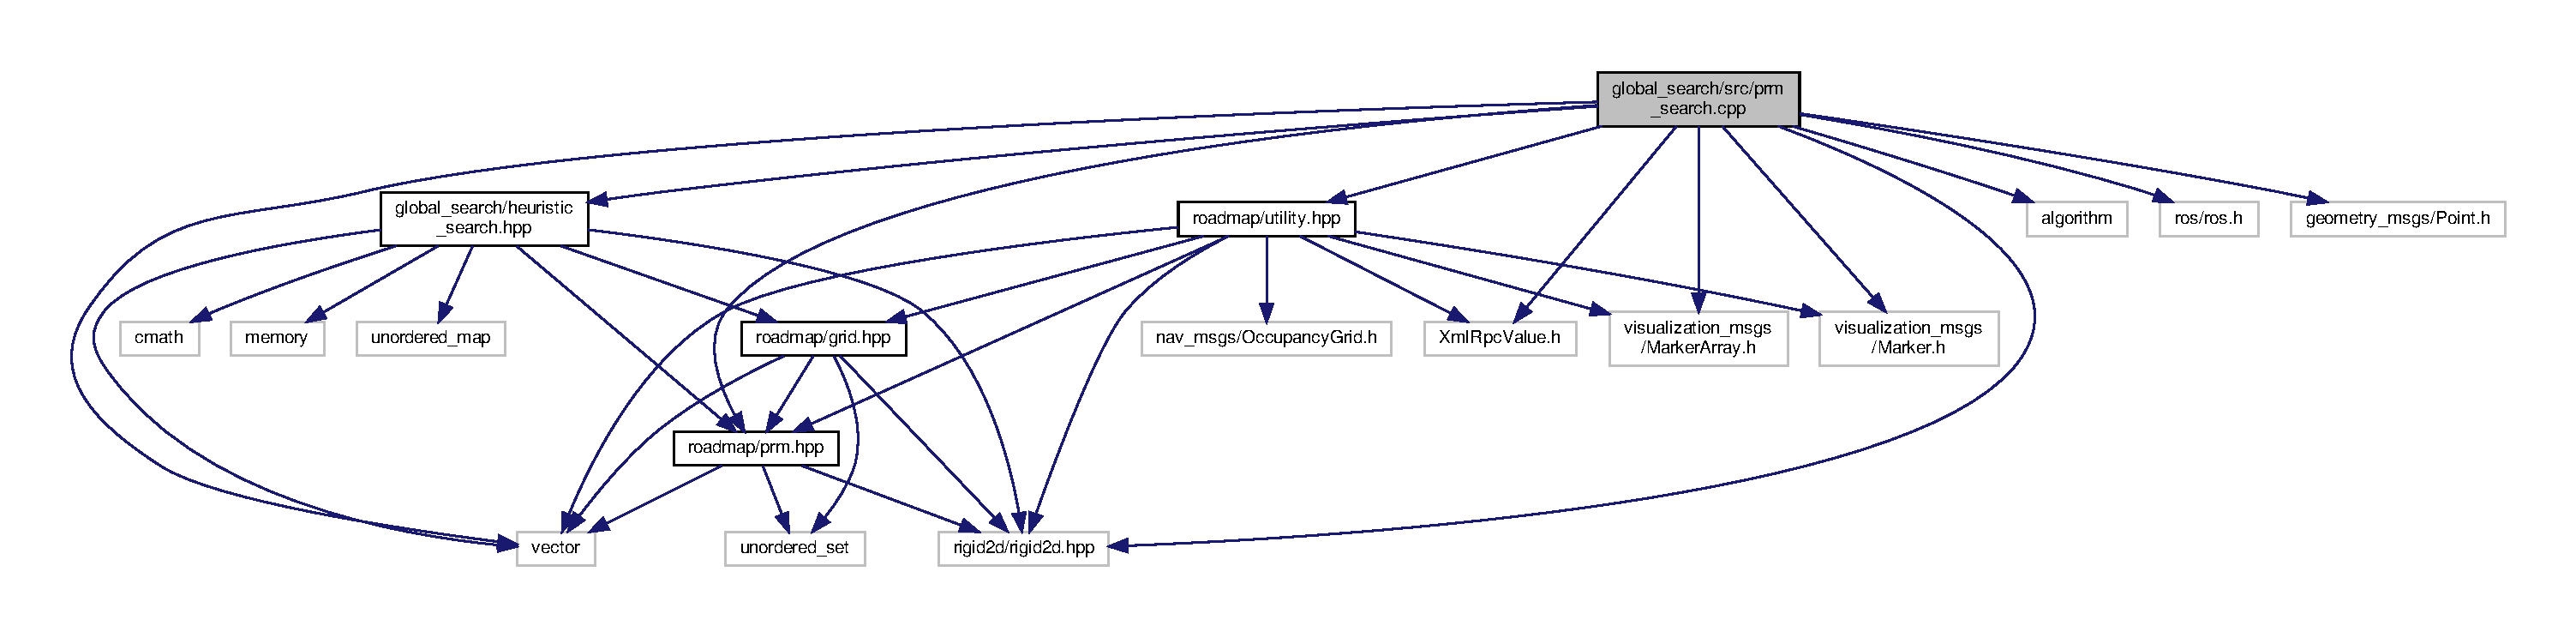
\includegraphics[width=350pt]{d7/d73/prm__search_8cpp__incl}
\end{center}
\end{figure}
\subsection*{Functions}
\begin{DoxyCompactItemize}
\item 
\mbox{\Hypertarget{prm__search_8cpp_a3c04138a5bfe5d72780bb7e82a18e627}\label{prm__search_8cpp_a3c04138a5bfe5d72780bb7e82a18e627}} 
int {\bfseries main} (int argc, char $\ast$$\ast$argv)
\end{DoxyCompactItemize}


\subsection{Detailed Description}
Node to create and draw a probabilistic road map. 

P\+A\+R\+A\+M\+E\+T\+E\+RS\+: obstacles (std\+::vector$<$std\+::vector$<$std\+::vector$<$double$>$) a vector of polygons represented by a vector of x,y coords for the verticies map\+\_\+x\+\_\+lims (std\+::vector$<$double$>$) \mbox{[}xmin, xmax\mbox{]} of the map map\+\_\+y\+\_\+lims (std\+::vector$<$double$>$) \mbox{[}ymin, ymax\mbox{]} of the map robot\+\_\+radius (double) buffer radius to avoid collisions with the robot body k\+\_\+nearest (unsigned int) number of neighboring verticies to match to graph\+\_\+size (unsigned int) number of nodes to use to build the graph r (std\+::vector$<$int$>$) color values g (std\+::vector$<$int$>$) color values b (std\+::vector$<$int$>$) color values 
\hypertarget{collision_8hpp}{}\section{roadmap/include/roadmap/collision.hpp File Reference}
\label{collision_8hpp}\index{roadmap/include/roadmap/collision.\+hpp@{roadmap/include/roadmap/collision.\+hpp}}


A library containing functions to detect various types of collisions.  


{\ttfamily \#include \char`\"{}rigid2d/rigid2d.\+hpp\char`\"{}}\newline
Include dependency graph for collision.\+hpp\+:\nopagebreak
\begin{figure}[H]
\begin{center}
\leavevmode
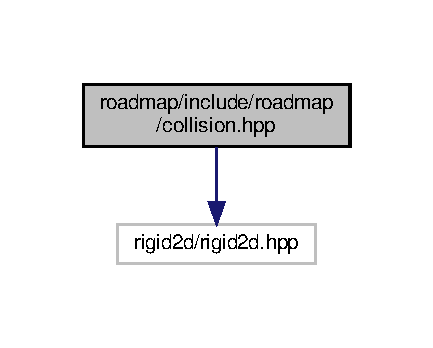
\includegraphics[width=208pt]{d9/d9b/collision_8hpp__incl}
\end{center}
\end{figure}
This graph shows which files directly or indirectly include this file\+:\nopagebreak
\begin{figure}[H]
\begin{center}
\leavevmode
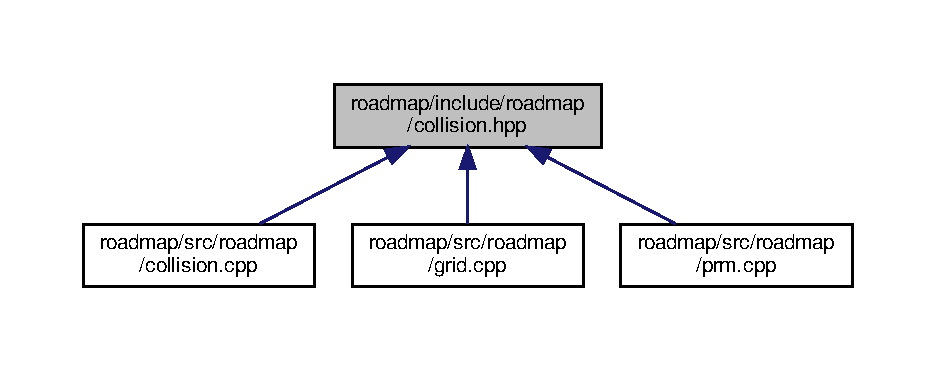
\includegraphics[width=350pt]{d2/d5b/collision_8hpp__dep__incl}
\end{center}
\end{figure}
\subsection*{Classes}
\begin{DoxyCompactItemize}
\item 
struct \hyperlink{structcollision_1_1DistRes}{collision\+::\+Dist\+Res}
\begin{DoxyCompactList}\small\item\em Used to return information from the point to line distance function. \end{DoxyCompactList}\end{DoxyCompactItemize}
\subsection*{Functions}
\begin{DoxyCompactItemize}
\item 
bool \hyperlink{collision_8hpp_aabf5aea7b02c454140c9bb242ca6e944}{collision\+::point\+\_\+to\+\_\+line\+\_\+distance} (rigid2d\+::\+Vector2D line\+\_\+start, rigid2d\+::\+Vector2D line\+\_\+end, rigid2d\+::\+Vector2D point, double threshold)
\begin{DoxyCompactList}\small\item\em Determine if a point is within a certain distance to a line. \end{DoxyCompactList}\item 
Dist\+Res \hyperlink{collision_8hpp_a7ac784d9a63acc273489e7e61c45416a}{collision\+::point\+\_\+to\+\_\+line\+\_\+distance} (rigid2d\+::\+Vector2D line\+\_\+start, rigid2d\+::\+Vector2D line\+\_\+end, rigid2d\+::\+Vector2D point)
\begin{DoxyCompactList}\small\item\em Calculate the minimum distance to a line segment. \end{DoxyCompactList}\item 
std\+::vector$<$ bool $>$ \hyperlink{collision_8hpp_af534ea532917e73ac2b28ca11c6cdf9f}{collision\+::point\+\_\+inside\+\_\+convex} (rigid2d\+::\+Vector2D point, std\+::vector$<$ rigid2d\+::\+Vector2D $>$ polygon, double buffer\+\_\+radius)
\begin{DoxyCompactList}\small\item\em Determine if a point is inside of a convex polygon, the points must be provided in order either cw or ccw. This function will account for connected the last vertex to the first vertex by appending the first vertex to the back of the vector. \end{DoxyCompactList}\item 
bool \hyperlink{collision_8hpp_a70c9083464a3dd4bc7c32dabe857e331}{collision\+::line\+\_\+shape\+\_\+intersection} (rigid2d\+::\+Vector2D line\+\_\+start, rigid2d\+::\+Vector2D line\+\_\+end, std\+::vector$<$ rigid2d\+::\+Vector2D $>$ polygon)
\begin{DoxyCompactList}\small\item\em Determine if a line segment intersects a convex polygon. \end{DoxyCompactList}\item 
bool \hyperlink{collision_8hpp_abf9b390bd1d767fe39f7d4806fae6b62}{collision\+::line\+\_\+shape\+\_\+intersection} (rigid2d\+::\+Vector2D line\+\_\+start, rigid2d\+::\+Vector2D line\+\_\+end, std\+::vector$<$ rigid2d\+::\+Vector2D $>$ polygon, double buffer\+\_\+radius)
\begin{DoxyCompactList}\small\item\em Determine if a line segment intersects a convex polygon or comes within a certain distance of it. This assumes the line start and end points are known to be outside of the buffer area of the polygon. \end{DoxyCompactList}\end{DoxyCompactItemize}


\subsection{Detailed Description}
A library containing functions to detect various types of collisions. 



\subsection{Function Documentation}
\mbox{\Hypertarget{collision_8hpp_file_a70c9083464a3dd4bc7c32dabe857e331}\label{collision_8hpp_file_a70c9083464a3dd4bc7c32dabe857e331}} 
\index{collision.\+hpp@{collision.\+hpp}!line\+\_\+shape\+\_\+intersection@{line\+\_\+shape\+\_\+intersection}}
\index{line\+\_\+shape\+\_\+intersection@{line\+\_\+shape\+\_\+intersection}!collision.\+hpp@{collision.\+hpp}}
\subsubsection{\texorpdfstring{line\+\_\+shape\+\_\+intersection()}{line\_shape\_intersection()}\hspace{0.1cm}{\footnotesize\ttfamily [1/2]}}
{\footnotesize\ttfamily bool collision\+::line\+\_\+shape\+\_\+intersection (\begin{DoxyParamCaption}\item[{rigid2d\+::\+Vector2D}]{line\+\_\+start,  }\item[{rigid2d\+::\+Vector2D}]{line\+\_\+end,  }\item[{std\+::vector$<$ rigid2d\+::\+Vector2D $>$}]{polygon }\end{DoxyParamCaption})}



Determine if a line segment intersects a convex polygon. 


\begin{DoxyParams}{Parameters}
{\em line\+\_\+start} & the point of the beginning of the line segment \\
\hline
{\em line\+\_\+end} & the point of the end of the line segment \\
\hline
{\em polygon} & a vector of verticies that define the polygon in ccw order \\
\hline
\end{DoxyParams}
\begin{DoxyReturn}{Returns}
True if there is an intersection between the line segment and polygon 
\end{DoxyReturn}
\mbox{\Hypertarget{collision_8hpp_file_abf9b390bd1d767fe39f7d4806fae6b62}\label{collision_8hpp_file_abf9b390bd1d767fe39f7d4806fae6b62}} 
\index{collision.\+hpp@{collision.\+hpp}!line\+\_\+shape\+\_\+intersection@{line\+\_\+shape\+\_\+intersection}}
\index{line\+\_\+shape\+\_\+intersection@{line\+\_\+shape\+\_\+intersection}!collision.\+hpp@{collision.\+hpp}}
\subsubsection{\texorpdfstring{line\+\_\+shape\+\_\+intersection()}{line\_shape\_intersection()}\hspace{0.1cm}{\footnotesize\ttfamily [2/2]}}
{\footnotesize\ttfamily bool collision\+::line\+\_\+shape\+\_\+intersection (\begin{DoxyParamCaption}\item[{rigid2d\+::\+Vector2D}]{line\+\_\+start,  }\item[{rigid2d\+::\+Vector2D}]{line\+\_\+end,  }\item[{std\+::vector$<$ rigid2d\+::\+Vector2D $>$}]{polygon,  }\item[{double}]{buffer\+\_\+radius }\end{DoxyParamCaption})}



Determine if a line segment intersects a convex polygon or comes within a certain distance of it. This assumes the line start and end points are known to be outside of the buffer area of the polygon. 


\begin{DoxyParams}{Parameters}
{\em line\+\_\+start} & the point of the beginning of the line segment \\
\hline
{\em line\+\_\+end} & the point of the end of the line segment \\
\hline
{\em polygon} & a vector of verticies that define the polygon in ccw order \\
\hline
{\em buffer\+\_\+radius} & a buffer distance to incorporate to the polygon boundary \\
\hline
\end{DoxyParams}
\begin{DoxyReturn}{Returns}
True if there is an intersection between the line segment and polygon or if the minimum distance to the line and shape is less than the buffer radius 
\end{DoxyReturn}
\mbox{\Hypertarget{collision_8hpp_file_af534ea532917e73ac2b28ca11c6cdf9f}\label{collision_8hpp_file_af534ea532917e73ac2b28ca11c6cdf9f}} 
\index{collision.\+hpp@{collision.\+hpp}!point\+\_\+inside\+\_\+convex@{point\+\_\+inside\+\_\+convex}}
\index{point\+\_\+inside\+\_\+convex@{point\+\_\+inside\+\_\+convex}!collision.\+hpp@{collision.\+hpp}}
\subsubsection{\texorpdfstring{point\+\_\+inside\+\_\+convex()}{point\_inside\_convex()}}
{\footnotesize\ttfamily std\+::vector$<$ bool $>$ collision\+::point\+\_\+inside\+\_\+convex (\begin{DoxyParamCaption}\item[{rigid2d\+::\+Vector2D}]{point,  }\item[{std\+::vector$<$ rigid2d\+::\+Vector2D $>$}]{polygon,  }\item[{double}]{buffer\+\_\+radius }\end{DoxyParamCaption})}



Determine if a point is inside of a convex polygon, the points must be provided in order either cw or ccw. This function will account for connected the last vertex to the first vertex by appending the first vertex to the back of the vector. 


\begin{DoxyParams}{Parameters}
{\em point} & the point to analyze \\
\hline
{\em polygon} & a vector of verticies that define the polygon in order, either cw or ccw. \\
\hline
{\em buffer\+\_\+radius} & a buffer distance to incorporate to the polygon boundary \\
\hline
\end{DoxyParams}
\begin{DoxyReturn}{Returns}
a 2 element vector, first element is true if there is a collision, second element describes the cause\+: True for inside the shape, False for outside the shape but in the buffer zone. 
\end{DoxyReturn}
\mbox{\Hypertarget{collision_8hpp_file_aabf5aea7b02c454140c9bb242ca6e944}\label{collision_8hpp_file_aabf5aea7b02c454140c9bb242ca6e944}} 
\index{collision.\+hpp@{collision.\+hpp}!point\+\_\+to\+\_\+line\+\_\+distance@{point\+\_\+to\+\_\+line\+\_\+distance}}
\index{point\+\_\+to\+\_\+line\+\_\+distance@{point\+\_\+to\+\_\+line\+\_\+distance}!collision.\+hpp@{collision.\+hpp}}
\subsubsection{\texorpdfstring{point\+\_\+to\+\_\+line\+\_\+distance()}{point\_to\_line\_distance()}\hspace{0.1cm}{\footnotesize\ttfamily [1/2]}}
{\footnotesize\ttfamily bool collision\+::point\+\_\+to\+\_\+line\+\_\+distance (\begin{DoxyParamCaption}\item[{rigid2d\+::\+Vector2D}]{line\+\_\+start,  }\item[{rigid2d\+::\+Vector2D}]{line\+\_\+end,  }\item[{rigid2d\+::\+Vector2D}]{point,  }\item[{double}]{threshold }\end{DoxyParamCaption})}



Determine if a point is within a certain distance to a line. 


\begin{DoxyParams}{Parameters}
{\em line\+\_\+start} & the point of the beginning of the line segment \\
\hline
{\em line\+\_\+end} & the point of the end of the line segment \\
\hline
{\em point} & the point to calculate the distance for \\
\hline
{\em threshold} & the distance threshold to compare against \\
\hline
\end{DoxyParams}
\begin{DoxyReturn}{Returns}
True if the distance between the point and the line is L\+E\+SS T\+H\+AN the provided threshold 
\end{DoxyReturn}
\mbox{\Hypertarget{collision_8hpp_file_a7ac784d9a63acc273489e7e61c45416a}\label{collision_8hpp_file_a7ac784d9a63acc273489e7e61c45416a}} 
\index{collision.\+hpp@{collision.\+hpp}!point\+\_\+to\+\_\+line\+\_\+distance@{point\+\_\+to\+\_\+line\+\_\+distance}}
\index{point\+\_\+to\+\_\+line\+\_\+distance@{point\+\_\+to\+\_\+line\+\_\+distance}!collision.\+hpp@{collision.\+hpp}}
\subsubsection{\texorpdfstring{point\+\_\+to\+\_\+line\+\_\+distance()}{point\_to\_line\_distance()}\hspace{0.1cm}{\footnotesize\ttfamily [2/2]}}
{\footnotesize\ttfamily Dist\+Res collision\+::point\+\_\+to\+\_\+line\+\_\+distance (\begin{DoxyParamCaption}\item[{rigid2d\+::\+Vector2D}]{line\+\_\+start,  }\item[{rigid2d\+::\+Vector2D}]{line\+\_\+end,  }\item[{rigid2d\+::\+Vector2D}]{point }\end{DoxyParamCaption})}



Calculate the minimum distance to a line segment. 


\begin{DoxyParams}{Parameters}
{\em line\+\_\+start} & the point of the beginning of the line segment \\
\hline
{\em line\+\_\+end} & the point of the end of the line segment \\
\hline
{\em point} & the point to calculate the distance for \\
\hline
\end{DoxyParams}
\begin{DoxyReturn}{Returns}
The shortest distance between the point and the line if the point is within the line segment or the minimum between the distances to the line\+\_\+start or line\+\_\+end 
\end{DoxyReturn}

\hypertarget{grid_8hpp}{}\section{roadmap/include/roadmap/grid.hpp File Reference}
\label{grid_8hpp}\index{roadmap/include/roadmap/grid.\+hpp@{roadmap/include/roadmap/grid.\+hpp}}


A library for building an occupancy grid.  


{\ttfamily \#include $<$vector$>$}\newline
{\ttfamily \#include $<$unordered\+\_\+set$>$}\newline
{\ttfamily \#include \char`\"{}rigid2d/rigid2d.\+hpp\char`\"{}}\newline
Include dependency graph for grid.\+hpp\+:\nopagebreak
\begin{figure}[H]
\begin{center}
\leavevmode
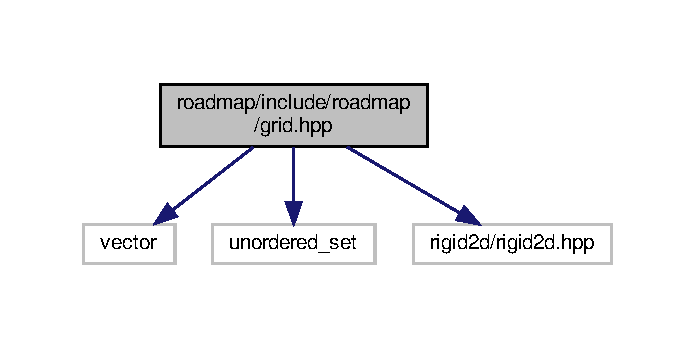
\includegraphics[width=334pt]{d7/da1/grid_8hpp__incl}
\end{center}
\end{figure}
This graph shows which files directly or indirectly include this file\+:\nopagebreak
\begin{figure}[H]
\begin{center}
\leavevmode
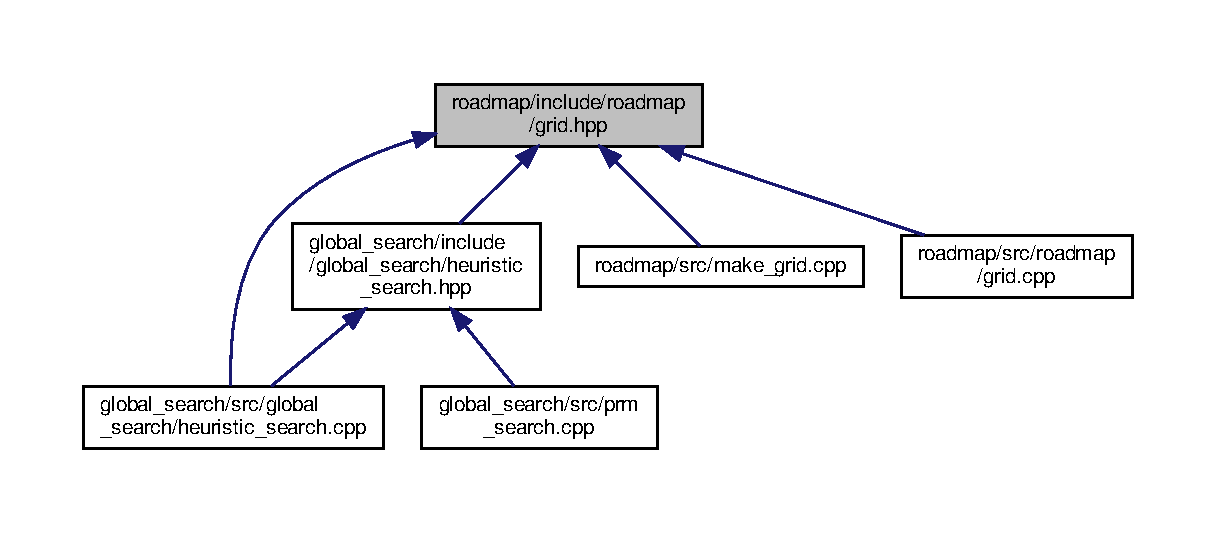
\includegraphics[width=208pt]{db/d6c/grid_8hpp__dep__incl}
\end{center}
\end{figure}
\subsection*{Classes}
\begin{DoxyCompactItemize}
\item 
struct \hyperlink{structgrid_1_1Map}{grid\+::\+Map}
\begin{DoxyCompactList}\small\item\em Contains information about a bound map. \end{DoxyCompactList}\item 
class \hyperlink{classgrid_1_1Grid}{grid\+::\+Grid}
\begin{DoxyCompactList}\small\item\em Class to create a \hyperlink{classgrid_1_1Grid}{Grid} overlay for provided \hyperlink{structgrid_1_1Map}{Map} information. \end{DoxyCompactList}\end{DoxyCompactItemize}


\subsection{Detailed Description}
A library for building an occupancy grid. 


\hypertarget{prm_8hpp}{}\section{roadmap/include/roadmap/prm.hpp File Reference}
\label{prm_8hpp}\index{roadmap/include/roadmap/prm.\+hpp@{roadmap/include/roadmap/prm.\+hpp}}


A library for building a Probabilistic Road Map.  


{\ttfamily \#include $<$vector$>$}\newline
{\ttfamily \#include $<$unordered\+\_\+set$>$}\newline
{\ttfamily \#include \char`\"{}rigid2d/rigid2d.\+hpp\char`\"{}}\newline
Include dependency graph for prm.\+hpp\+:
\nopagebreak
\begin{figure}[H]
\begin{center}
\leavevmode
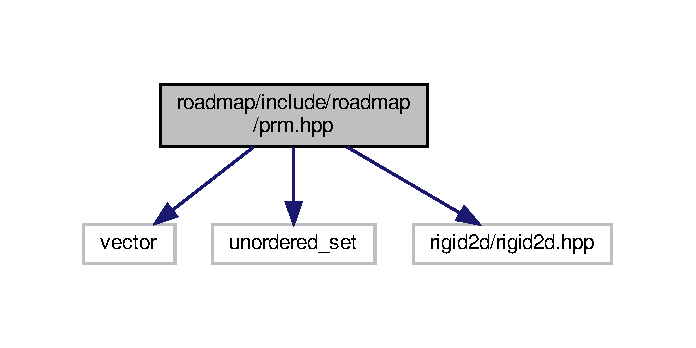
\includegraphics[width=334pt]{d7/d00/prm_8hpp__incl}
\end{center}
\end{figure}
This graph shows which files directly or indirectly include this file\+:
\nopagebreak
\begin{figure}[H]
\begin{center}
\leavevmode
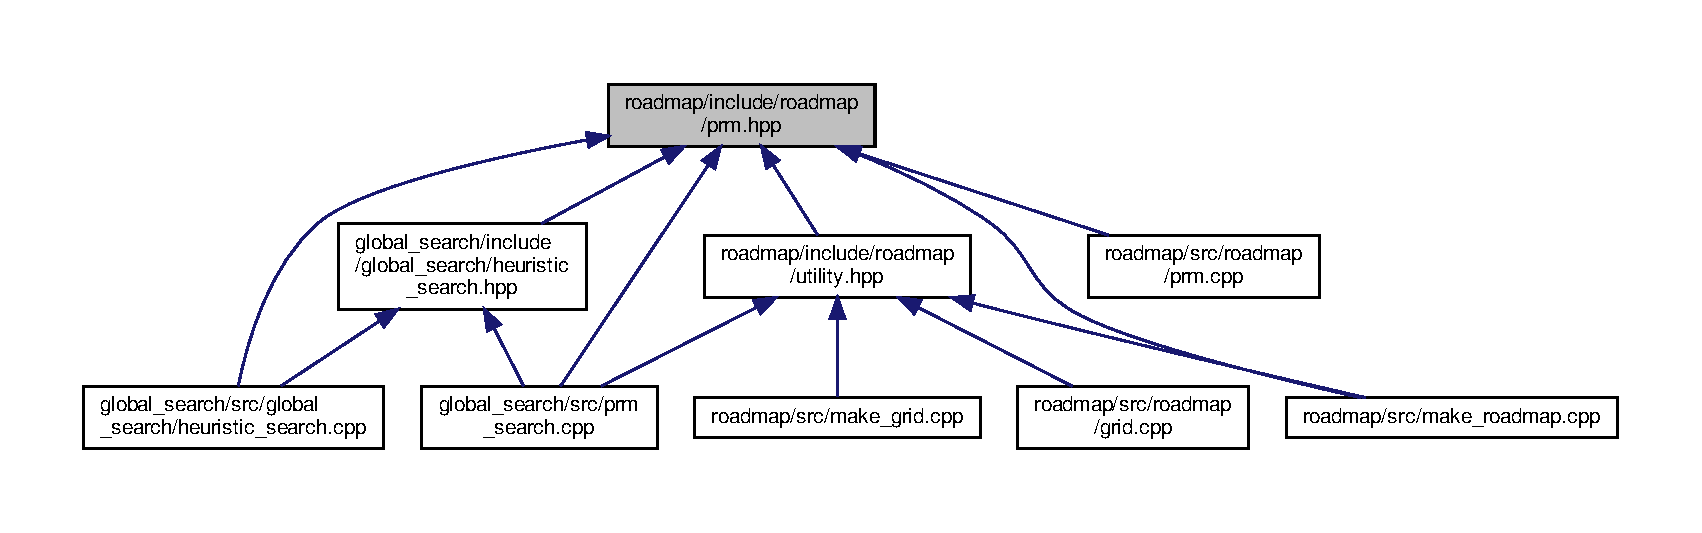
\includegraphics[width=350pt]{d6/d45/prm_8hpp__dep__incl}
\end{center}
\end{figure}
\subsection*{Classes}
\begin{DoxyCompactItemize}
\item 
struct \hyperlink{structprm_1_1Edge}{prm\+::\+Edge}
\begin{DoxyCompactList}\small\item\em A struct to fully describe a connection between two nodes. \end{DoxyCompactList}\item 
struct \hyperlink{structprm_1_1Node}{prm\+::\+Node}
\begin{DoxyCompactList}\small\item\em A struct to define a node and interact with it. \end{DoxyCompactList}\item 
class \hyperlink{classprm_1_1RoadMap}{prm\+::\+Road\+Map}
\begin{DoxyCompactList}\small\item\em A class to build a Probabilistic Road Maps based on provided Map information. \end{DoxyCompactList}\end{DoxyCompactItemize}


\subsection{Detailed Description}
A library for building a Probabilistic Road Map. 


\hypertarget{utility_8hpp}{}\section{roadmap/include/roadmap/utility.hpp File Reference}
\label{utility_8hpp}\index{roadmap/include/roadmap/utility.\+hpp@{roadmap/include/roadmap/utility.\+hpp}}


A library of utility functions for the various nodes and libraries of this package.  


{\ttfamily \#include $<$vector$>$}\newline
{\ttfamily \#include $<$Xml\+Rpc\+Value.\+h$>$}\newline
{\ttfamily \#include \char`\"{}rigid2d/rigid2d.\+hpp\char`\"{}}\newline
Include dependency graph for utility.\+hpp\+:
\nopagebreak
\begin{figure}[H]
\begin{center}
\leavevmode
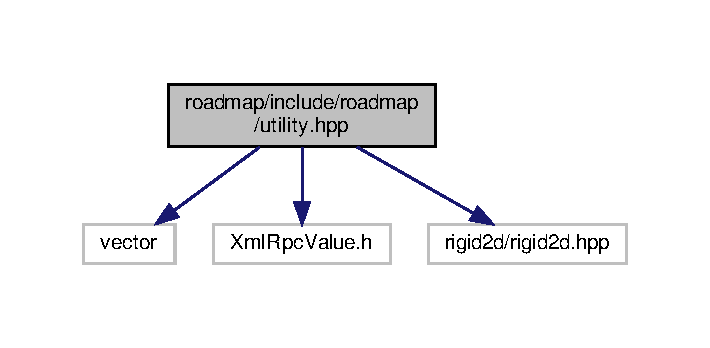
\includegraphics[width=341pt]{d1/d48/utility_8hpp__incl}
\end{center}
\end{figure}
This graph shows which files directly or indirectly include this file\+:
\nopagebreak
\begin{figure}[H]
\begin{center}
\leavevmode
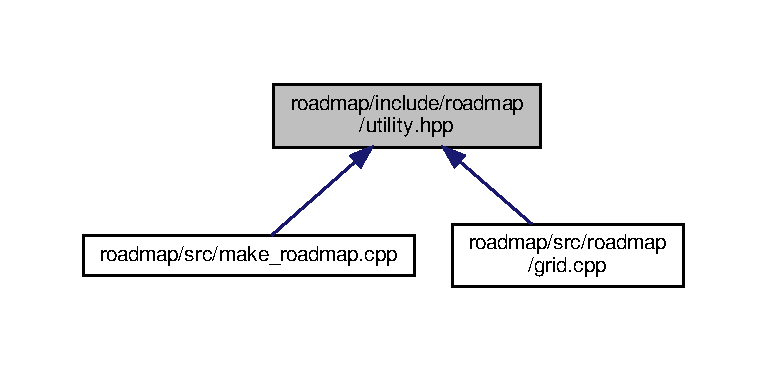
\includegraphics[width=350pt]{d7/d68/utility_8hpp__dep__incl}
\end{center}
\end{figure}
\subsection*{Functions}
\begin{DoxyCompactItemize}
\item 
std\+::vector$<$ std\+::vector$<$ rigid2d\+::\+Vector2D $>$ $>$ \hyperlink{utility_8hpp_a146978c7eb3e5b6e8604499596442f9e}{utility\+::parse\+\_\+obstacle\+\_\+data} (Xml\+Rpc\+::\+Xml\+Rpc\+Value obstacles, double cell\+\_\+size)
\begin{DoxyCompactList}\small\item\em converts obstacle data from a Y\+A\+ML file into a vector of vectors. T\+O\+DO\+: changes this to a template based output \end{DoxyCompactList}\item 
std\+::vector$<$ rigid2d\+::\+Vector2D $>$ \hyperlink{utility_8hpp_a9eb7f849405aea8fd6215f962f7d77a2}{utility\+::create\+\_\+map\+\_\+vector} (std\+::vector$<$ double $>$ map\+\_\+x\+\_\+lims, std\+::vector$<$ double $>$ map\+\_\+y\+\_\+lims)
\begin{DoxyCompactList}\small\item\em gerenate a vector of the 4 map verticies \end{DoxyCompactList}\end{DoxyCompactItemize}


\subsection{Detailed Description}
A library of utility functions for the various nodes and libraries of this package. 



\subsection{Function Documentation}
\mbox{\Hypertarget{utility_8hpp_file_a9eb7f849405aea8fd6215f962f7d77a2}\label{utility_8hpp_file_a9eb7f849405aea8fd6215f962f7d77a2}} 
\index{utility.\+hpp@{utility.\+hpp}!create\+\_\+map\+\_\+vector@{create\+\_\+map\+\_\+vector}}
\index{create\+\_\+map\+\_\+vector@{create\+\_\+map\+\_\+vector}!utility.\+hpp@{utility.\+hpp}}
\subsubsection{\texorpdfstring{create\+\_\+map\+\_\+vector()}{create\_map\_vector()}}
{\footnotesize\ttfamily std\+::vector$<$ rigid2d\+::\+Vector2D $>$ utility\+::create\+\_\+map\+\_\+vector (\begin{DoxyParamCaption}\item[{std\+::vector$<$ double $>$}]{map\+\_\+x\+\_\+lims,  }\item[{std\+::vector$<$ double $>$}]{map\+\_\+y\+\_\+lims }\end{DoxyParamCaption})}



gerenate a vector of the 4 map verticies 


\begin{DoxyParams}{Parameters}
{\em map\+\_\+x\+\_\+lims} & the x axis limits of the map \\
\hline
{\em map\+\_\+y\+\_\+lims} & the y axis limits of the map \\
\hline
\end{DoxyParams}
\begin{DoxyReturn}{Returns}
a vector of the map verticies in ccw order 
\end{DoxyReturn}
\mbox{\Hypertarget{utility_8hpp_file_a146978c7eb3e5b6e8604499596442f9e}\label{utility_8hpp_file_a146978c7eb3e5b6e8604499596442f9e}} 
\index{utility.\+hpp@{utility.\+hpp}!parse\+\_\+obstacle\+\_\+data@{parse\+\_\+obstacle\+\_\+data}}
\index{parse\+\_\+obstacle\+\_\+data@{parse\+\_\+obstacle\+\_\+data}!utility.\+hpp@{utility.\+hpp}}
\subsubsection{\texorpdfstring{parse\+\_\+obstacle\+\_\+data()}{parse\_obstacle\_data()}}
{\footnotesize\ttfamily std\+::vector$<$ std\+::vector$<$ rigid2d\+::\+Vector2D $>$ $>$ utility\+::parse\+\_\+obstacle\+\_\+data (\begin{DoxyParamCaption}\item[{Xml\+Rpc\+::\+Xml\+Rpc\+Value}]{obstacles,  }\item[{double}]{cell\+\_\+size }\end{DoxyParamCaption})}



converts obstacle data from a Y\+A\+ML file into a vector of vectors. T\+O\+DO\+: changes this to a template based output 


\begin{DoxyParams}{Parameters}
{\em obstacles} & the a list of lists containing obstacle vertices \\
\hline
{\em cell\+\_\+size} & a scaling factor to apply to the vertex coordinates. Use 1 if you do not want to scale them. \\
\hline
\end{DoxyParams}
\begin{DoxyReturn}{Returns}
a vector of vectors containing obstacle vertices 
\end{DoxyReturn}

\hypertarget{draw__world_8cpp}{}\section{roadmap/src/draw\+\_\+world.cpp File Reference}
\label{draw__world_8cpp}\index{roadmap/src/draw\+\_\+world.\+cpp@{roadmap/src/draw\+\_\+world.\+cpp}}


Node to draw the features of the real world map.  


{\ttfamily \#include $<$vector$>$}\newline
{\ttfamily \#include $<$Xml\+Rpc\+Value.\+h$>$}\newline
{\ttfamily \#include $<$ros/ros.\+h$>$}\newline
{\ttfamily \#include \char`\"{}geometry\+\_\+msgs/\+Point.\+h\char`\"{}}\newline
{\ttfamily \#include \char`\"{}visualization\+\_\+msgs/\+Marker\+Array.\+h\char`\"{}}\newline
{\ttfamily \#include \char`\"{}visualization\+\_\+msgs/\+Marker.\+h\char`\"{}}\newline
{\ttfamily \#include \char`\"{}rigid2d/rigid2d.\+hpp\char`\"{}}\newline
Include dependency graph for draw\+\_\+world.\+cpp\+:
\nopagebreak
\begin{figure}[H]
\begin{center}
\leavevmode
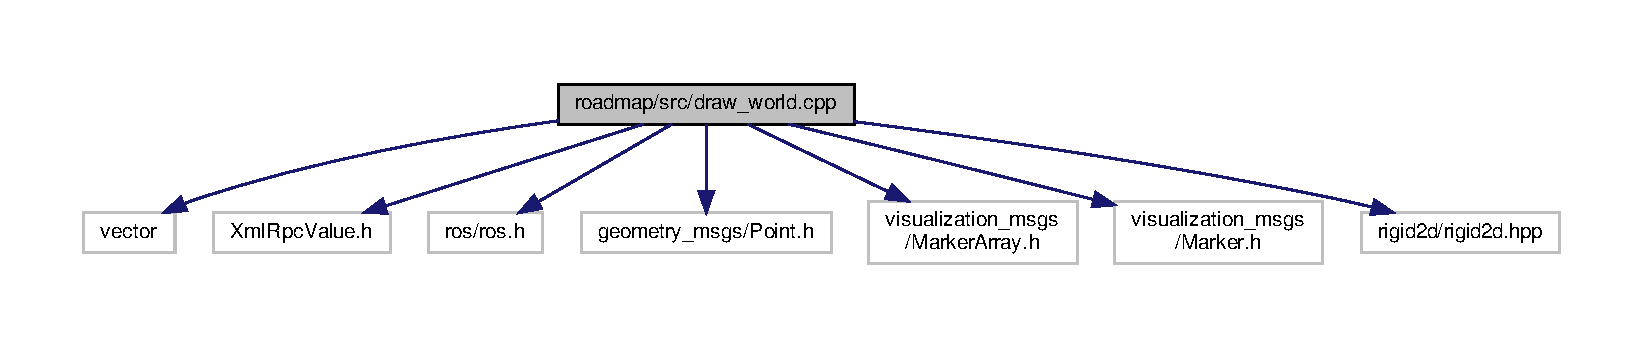
\includegraphics[width=350pt]{d2/dd7/draw__world_8cpp__incl}
\end{center}
\end{figure}
\subsection*{Functions}
\begin{DoxyCompactItemize}
\item 
\mbox{\Hypertarget{draw__world_8cpp_a3c04138a5bfe5d72780bb7e82a18e627}\label{draw__world_8cpp_a3c04138a5bfe5d72780bb7e82a18e627}} 
int {\bfseries main} (int argc, char $\ast$$\ast$argv)
\end{DoxyCompactItemize}


\subsection{Detailed Description}
Node to draw the features of the real world map. 

P\+A\+R\+A\+M\+E\+T\+E\+RS\+: obstacles (std\+::vector$<$std\+::vector$<$std\+::vector$<$double$>$) a vector of polygons represented by a vector of x,y coords for the verticies map\+\_\+x\+\_\+lims (std\+::vector$<$double$>$) \mbox{[}xmin, xmax\mbox{]} of the map map\+\_\+y\+\_\+lims (std\+::vector$<$double$>$) \mbox{[}ymin, ymax\mbox{]} of the map r (std\+::vector$<$int$>$) color values g (std\+::vector$<$int$>$) color values b (std\+::vector$<$int$>$) color values P\+U\+B\+L\+I\+S\+H\+ES\+: /visualization\+\_\+marker\+\_\+array (visualization\+\_\+msgs\+::\+Marker\+Array) markers 
\hypertarget{make__grid_8cpp}{}\section{roadmap/src/make\+\_\+grid.cpp File Reference}
\label{make__grid_8cpp}\index{roadmap/src/make\+\_\+grid.\+cpp@{roadmap/src/make\+\_\+grid.\+cpp}}


Node to create and draw a grid.  


{\ttfamily \#include $<$vector$>$}\newline
{\ttfamily \#include $<$algorithm$>$}\newline
{\ttfamily \#include $<$Xml\+Rpc\+Value.\+h$>$}\newline
{\ttfamily \#include $<$ros/ros.\+h$>$}\newline
{\ttfamily \#include \char`\"{}nav\+\_\+msgs/\+Occupancy\+Grid.\+h\char`\"{}}\newline
{\ttfamily \#include \char`\"{}rigid2d/rigid2d.\+hpp\char`\"{}}\newline
{\ttfamily \#include \char`\"{}roadmap/grid.\+hpp\char`\"{}}\newline
{\ttfamily \#include \char`\"{}roadmap/utility.\+hpp\char`\"{}}\newline
Include dependency graph for make\+\_\+grid.\+cpp\+:
\nopagebreak
\begin{figure}[H]
\begin{center}
\leavevmode
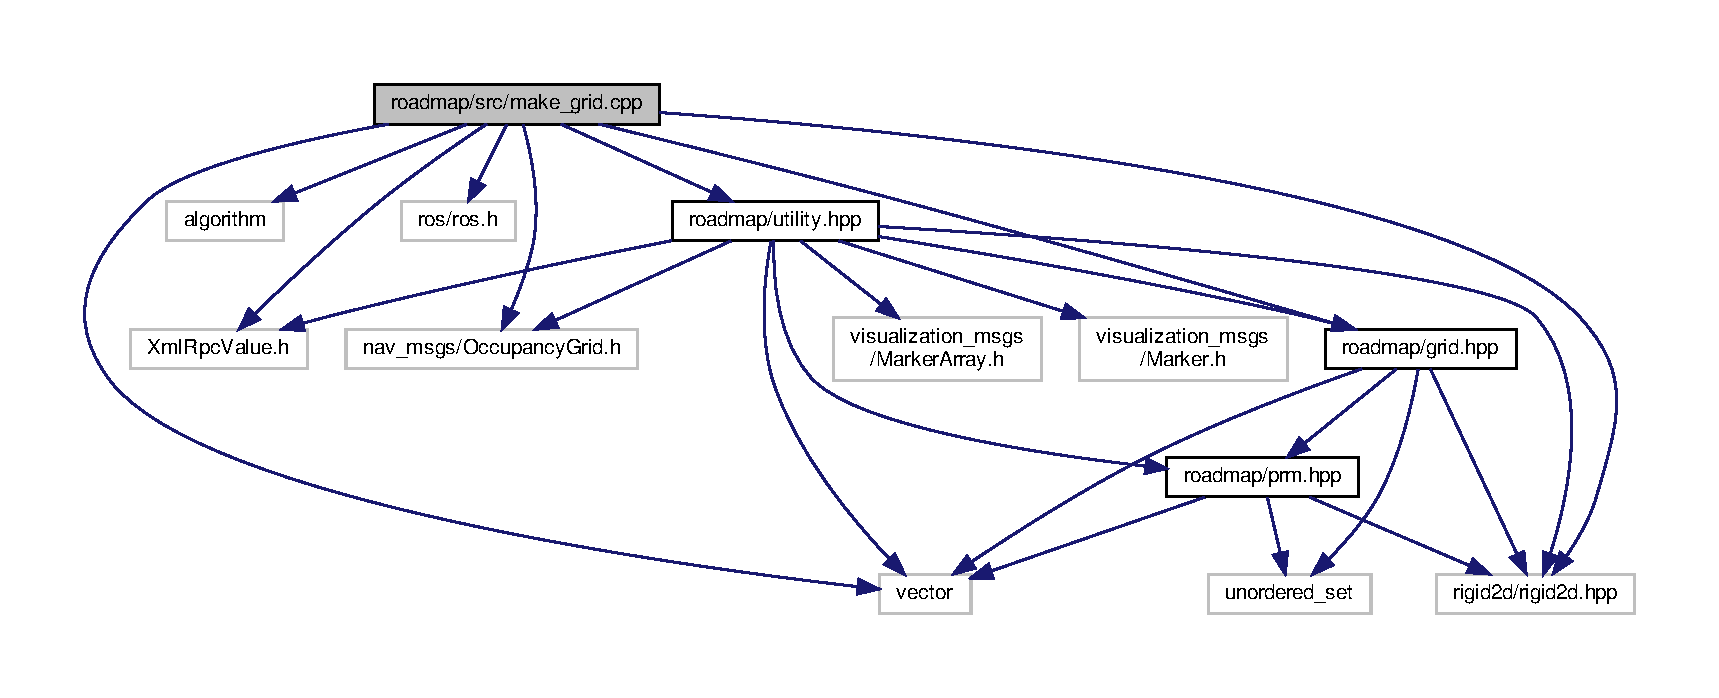
\includegraphics[width=350pt]{dc/d24/make__grid_8cpp__incl}
\end{center}
\end{figure}
\subsection*{Functions}
\begin{DoxyCompactItemize}
\item 
\mbox{\Hypertarget{make__grid_8cpp_a3c04138a5bfe5d72780bb7e82a18e627}\label{make__grid_8cpp_a3c04138a5bfe5d72780bb7e82a18e627}} 
int {\bfseries main} (int argc, char $\ast$$\ast$argv)
\end{DoxyCompactItemize}


\subsection{Detailed Description}
Node to create and draw a grid. 

P\+A\+R\+A\+M\+E\+T\+E\+RS\+: obstacles (std\+::vector$<$std\+::vector$<$std\+::vector$<$double$>$) a vector of polygons represented by a vector of x,y coords for the verticies map\+\_\+x\+\_\+lims (std\+::vector$<$double$>$) \mbox{[}xmin, xmax\mbox{]} of the map map\+\_\+y\+\_\+lims (std\+::vector$<$double$>$) \mbox{[}ymin, ymax\mbox{]} of the map robot\+\_\+radius (double) buffer radius to avoid collisions with the robot body cell\+\_\+size (double) scaling factor for the map grid\+\_\+res (double) scaling factor for the grid cell size P\+U\+B\+L\+I\+S\+H\+ES\+: /visualization\+\_\+marker\+\_\+array (visualization\+\_\+msgs\+::\+Marker\+Array) markers 
\hypertarget{make__roadmap_8cpp}{}\section{roadmap/src/make\+\_\+roadmap.cpp File Reference}
\label{make__roadmap_8cpp}\index{roadmap/src/make\+\_\+roadmap.\+cpp@{roadmap/src/make\+\_\+roadmap.\+cpp}}


Node to create and draw a probabilistic road map.  


{\ttfamily \#include $<$vector$>$}\newline
{\ttfamily \#include $<$algorithm$>$}\newline
{\ttfamily \#include $<$Xml\+Rpc\+Value.\+h$>$}\newline
{\ttfamily \#include $<$ros/ros.\+h$>$}\newline
{\ttfamily \#include \char`\"{}geometry\+\_\+msgs/\+Point.\+h\char`\"{}}\newline
{\ttfamily \#include \char`\"{}visualization\+\_\+msgs/\+Marker\+Array.\+h\char`\"{}}\newline
{\ttfamily \#include \char`\"{}visualization\+\_\+msgs/\+Marker.\+h\char`\"{}}\newline
{\ttfamily \#include \char`\"{}rigid2d/rigid2d.\+hpp\char`\"{}}\newline
{\ttfamily \#include \char`\"{}roadmap/prm.\+hpp\char`\"{}}\newline
{\ttfamily \#include \char`\"{}roadmap/utility.\+hpp\char`\"{}}\newline
Include dependency graph for make\+\_\+roadmap.\+cpp\+:
\nopagebreak
\begin{figure}[H]
\begin{center}
\leavevmode
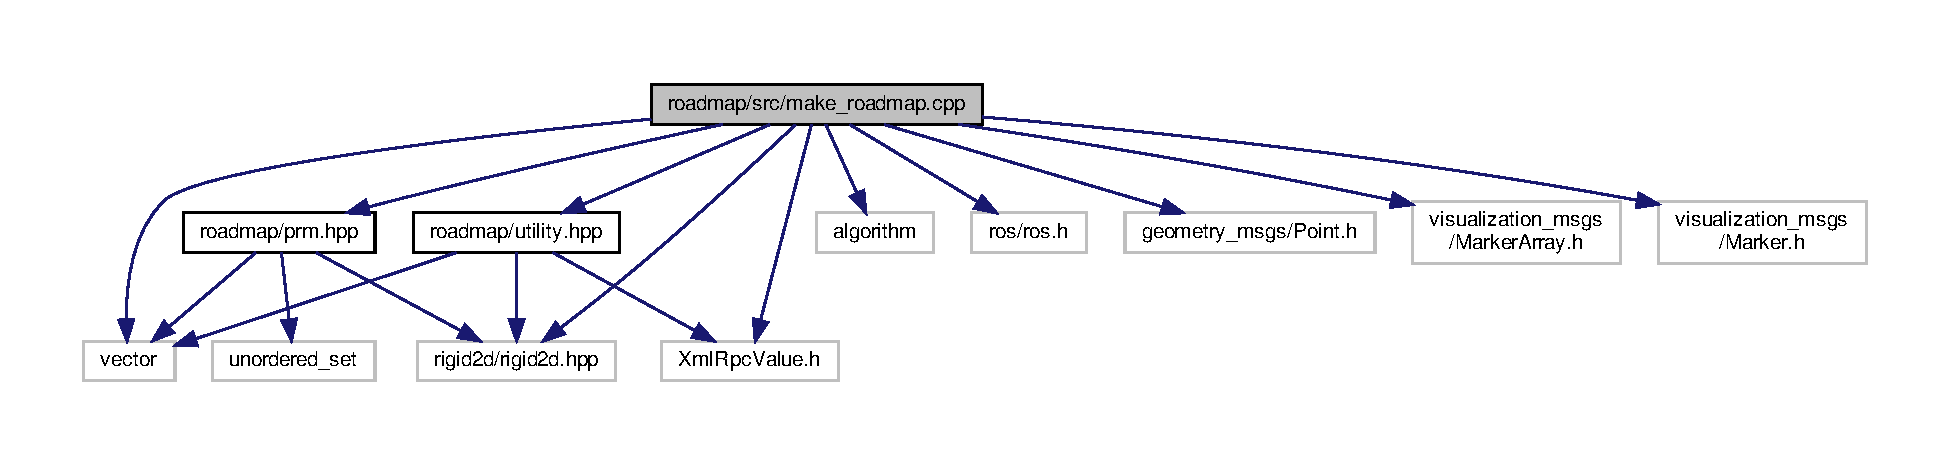
\includegraphics[width=350pt]{df/d6e/make__roadmap_8cpp__incl}
\end{center}
\end{figure}
\subsection*{Functions}
\begin{DoxyCompactItemize}
\item 
\mbox{\Hypertarget{make__roadmap_8cpp_a3c04138a5bfe5d72780bb7e82a18e627}\label{make__roadmap_8cpp_a3c04138a5bfe5d72780bb7e82a18e627}} 
int {\bfseries main} (int argc, char $\ast$$\ast$argv)
\end{DoxyCompactItemize}


\subsection{Detailed Description}
Node to create and draw a probabilistic road map. 

P\+A\+R\+A\+M\+E\+T\+E\+RS\+: obstacles (std\+::vector$<$std\+::vector$<$std\+::vector$<$double$>$) a vector of polygons represented by a vector of x,y coords for the verticies map\+\_\+x\+\_\+lims (std\+::vector$<$double$>$) \mbox{[}xmin, xmax\mbox{]} of the map map\+\_\+y\+\_\+lims (std\+::vector$<$double$>$) \mbox{[}ymin, ymax\mbox{]} of the map robot\+\_\+radius (double) buffer radius to avoid collisions with the robot body k\+\_\+nearest (unsigned int) number of neighboring verticies to match to graph\+\_\+size (unsigned int) number of nodes to use to build the graph r (std\+::vector$<$int$>$) color values g (std\+::vector$<$int$>$) color values b (std\+::vector$<$int$>$) color values P\+U\+B\+L\+I\+S\+H\+ES\+: /visualization\+\_\+marker\+\_\+array (visualization\+\_\+msgs\+::\+Marker\+Array) markers 
\hypertarget{collision_8cpp}{}\section{roadmap/src/roadmap/collision.cpp File Reference}
\label{collision_8cpp}\index{roadmap/src/roadmap/collision.\+cpp@{roadmap/src/roadmap/collision.\+cpp}}


A library containing functions to detect various types of collisions.  


{\ttfamily \#include $<$algorithm$>$}\newline
{\ttfamily \#include $<$functional$>$}\newline
{\ttfamily \#include $<$iostream$>$}\newline
{\ttfamily \#include $<$vector$>$}\newline
{\ttfamily \#include \char`\"{}roadmap/collision.\+hpp\char`\"{}}\newline
{\ttfamily \#include \char`\"{}rigid2d/rigid2d.\+hpp\char`\"{}}\newline
Include dependency graph for collision.\+cpp\+:
\nopagebreak
\begin{figure}[H]
\begin{center}
\leavevmode
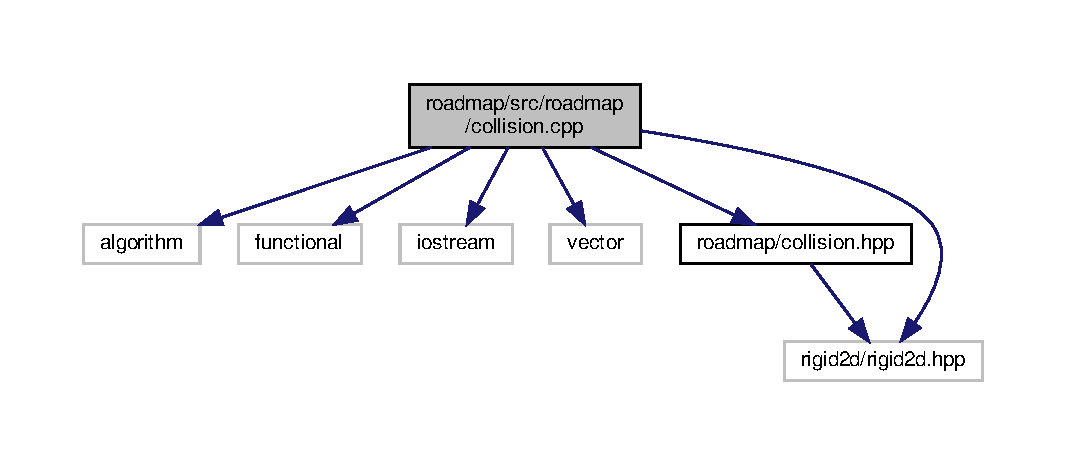
\includegraphics[width=350pt]{d9/d5a/collision_8cpp__incl}
\end{center}
\end{figure}
\subsection*{Functions}
\begin{DoxyCompactItemize}
\item 
Dist\+Res \hyperlink{collision_8hpp_a7ac784d9a63acc273489e7e61c45416a}{collision\+::point\+\_\+to\+\_\+line\+\_\+distance} (rigid2d\+::\+Vector2D line\+\_\+start, rigid2d\+::\+Vector2D line\+\_\+end, rigid2d\+::\+Vector2D point)
\begin{DoxyCompactList}\small\item\em Determine if a point is within a certain distance to a line. \end{DoxyCompactList}\item 
bool \hyperlink{collision_8hpp_aabf5aea7b02c454140c9bb242ca6e944}{collision\+::point\+\_\+to\+\_\+line\+\_\+distance} (rigid2d\+::\+Vector2D line\+\_\+start, rigid2d\+::\+Vector2D line\+\_\+end, rigid2d\+::\+Vector2D point, double threshold)
\begin{DoxyCompactList}\small\item\em Determine if a point is within a certain distance to a line. \end{DoxyCompactList}\item 
std\+::vector$<$ bool $>$ \hyperlink{collision_8hpp_af534ea532917e73ac2b28ca11c6cdf9f}{collision\+::point\+\_\+inside\+\_\+convex} (rigid2d\+::\+Vector2D point, std\+::vector$<$ rigid2d\+::\+Vector2D $>$ polygon, double buffer\+\_\+radius)
\begin{DoxyCompactList}\small\item\em Determine if a point is inside of a convex polygon, the points must be provided in order either cw or ccw. This function will account for connected the last vertex to the first vertex by appending the first vertex to the back of the vector. \end{DoxyCompactList}\item 
bool \hyperlink{collision_8hpp_a70c9083464a3dd4bc7c32dabe857e331}{collision\+::line\+\_\+shape\+\_\+intersection} (rigid2d\+::\+Vector2D line\+\_\+start, rigid2d\+::\+Vector2D line\+\_\+end, std\+::vector$<$ rigid2d\+::\+Vector2D $>$ polygon)
\begin{DoxyCompactList}\small\item\em Determine if a line segment intersects a convex polygon. \end{DoxyCompactList}\item 
bool \hyperlink{collision_8hpp_abf9b390bd1d767fe39f7d4806fae6b62}{collision\+::line\+\_\+shape\+\_\+intersection} (rigid2d\+::\+Vector2D line\+\_\+start, rigid2d\+::\+Vector2D line\+\_\+end, std\+::vector$<$ rigid2d\+::\+Vector2D $>$ polygon, double buffer\+\_\+radius)
\begin{DoxyCompactList}\small\item\em Determine if a line segment intersects a convex polygon or comes within a certain distance of it. This assumes the line start and end points are known to be outside of the buffer area of the polygon. \end{DoxyCompactList}\end{DoxyCompactItemize}


\subsection{Detailed Description}
A library containing functions to detect various types of collisions. 



\subsection{Function Documentation}
\mbox{\Hypertarget{collision_8hpp_file_a70c9083464a3dd4bc7c32dabe857e331}\label{collision_8hpp_file_a70c9083464a3dd4bc7c32dabe857e331}} 
\index{collision.\+cpp@{collision.\+cpp}!line\+\_\+shape\+\_\+intersection@{line\+\_\+shape\+\_\+intersection}}
\index{line\+\_\+shape\+\_\+intersection@{line\+\_\+shape\+\_\+intersection}!collision.\+cpp@{collision.\+cpp}}
\subsubsection{\texorpdfstring{line\+\_\+shape\+\_\+intersection()}{line\_shape\_intersection()}\hspace{0.1cm}{\footnotesize\ttfamily [1/2]}}
{\footnotesize\ttfamily bool collision\+::line\+\_\+shape\+\_\+intersection (\begin{DoxyParamCaption}\item[{rigid2d\+::\+Vector2D}]{line\+\_\+start,  }\item[{rigid2d\+::\+Vector2D}]{line\+\_\+end,  }\item[{std\+::vector$<$ rigid2d\+::\+Vector2D $>$}]{polygon }\end{DoxyParamCaption})}



Determine if a line segment intersects a convex polygon. 


\begin{DoxyParams}{Parameters}
{\em line\+\_\+start} & the point of the beginning of the line segment \\
\hline
{\em line\+\_\+end} & the point of the end of the line segment \\
\hline
{\em polygon} & a vector of verticies that define the polygon in ccw order \\
\hline
\end{DoxyParams}
\begin{DoxyReturn}{Returns}
True if there is an intersection between the line segment and polygon 
\end{DoxyReturn}
\mbox{\Hypertarget{collision_8hpp_file_abf9b390bd1d767fe39f7d4806fae6b62}\label{collision_8hpp_file_abf9b390bd1d767fe39f7d4806fae6b62}} 
\index{collision.\+cpp@{collision.\+cpp}!line\+\_\+shape\+\_\+intersection@{line\+\_\+shape\+\_\+intersection}}
\index{line\+\_\+shape\+\_\+intersection@{line\+\_\+shape\+\_\+intersection}!collision.\+cpp@{collision.\+cpp}}
\subsubsection{\texorpdfstring{line\+\_\+shape\+\_\+intersection()}{line\_shape\_intersection()}\hspace{0.1cm}{\footnotesize\ttfamily [2/2]}}
{\footnotesize\ttfamily bool collision\+::line\+\_\+shape\+\_\+intersection (\begin{DoxyParamCaption}\item[{rigid2d\+::\+Vector2D}]{line\+\_\+start,  }\item[{rigid2d\+::\+Vector2D}]{line\+\_\+end,  }\item[{std\+::vector$<$ rigid2d\+::\+Vector2D $>$}]{polygon,  }\item[{double}]{buffer\+\_\+radius }\end{DoxyParamCaption})}



Determine if a line segment intersects a convex polygon or comes within a certain distance of it. This assumes the line start and end points are known to be outside of the buffer area of the polygon. 


\begin{DoxyParams}{Parameters}
{\em line\+\_\+start} & the point of the beginning of the line segment \\
\hline
{\em line\+\_\+end} & the point of the end of the line segment \\
\hline
{\em polygon} & a vector of verticies that define the polygon in ccw order \\
\hline
{\em buffer\+\_\+radius} & a buffer distance to incorporate to the polygon boundary \\
\hline
\end{DoxyParams}
\begin{DoxyReturn}{Returns}
True if there is an intersection between the line segment and polygon or if the minimum distance to the line and shape is less than the buffer radius 
\end{DoxyReturn}
\mbox{\Hypertarget{collision_8hpp_file_af534ea532917e73ac2b28ca11c6cdf9f}\label{collision_8hpp_file_af534ea532917e73ac2b28ca11c6cdf9f}} 
\index{collision.\+cpp@{collision.\+cpp}!point\+\_\+inside\+\_\+convex@{point\+\_\+inside\+\_\+convex}}
\index{point\+\_\+inside\+\_\+convex@{point\+\_\+inside\+\_\+convex}!collision.\+cpp@{collision.\+cpp}}
\subsubsection{\texorpdfstring{point\+\_\+inside\+\_\+convex()}{point\_inside\_convex()}}
{\footnotesize\ttfamily std\+::vector$<$ bool $>$ collision\+::point\+\_\+inside\+\_\+convex (\begin{DoxyParamCaption}\item[{rigid2d\+::\+Vector2D}]{point,  }\item[{std\+::vector$<$ rigid2d\+::\+Vector2D $>$}]{polygon,  }\item[{double}]{buffer\+\_\+radius }\end{DoxyParamCaption})}



Determine if a point is inside of a convex polygon, the points must be provided in order either cw or ccw. This function will account for connected the last vertex to the first vertex by appending the first vertex to the back of the vector. 


\begin{DoxyParams}{Parameters}
{\em point} & the point to analyze \\
\hline
{\em polygon} & a vector of verticies that define the polygon in order, either cw or ccw. \\
\hline
{\em buffer\+\_\+radius} & a buffer distance to incorporate to the polygon boundary \\
\hline
\end{DoxyParams}
\begin{DoxyReturn}{Returns}
a 2 element vector, first element is true if there is a collision, second element describes the cause\+: True for inside the shape, False for outside the shape, but in the buffer zone. 
\end{DoxyReturn}
\mbox{\Hypertarget{collision_8hpp_file_aabf5aea7b02c454140c9bb242ca6e944}\label{collision_8hpp_file_aabf5aea7b02c454140c9bb242ca6e944}} 
\index{collision.\+cpp@{collision.\+cpp}!point\+\_\+to\+\_\+line\+\_\+distance@{point\+\_\+to\+\_\+line\+\_\+distance}}
\index{point\+\_\+to\+\_\+line\+\_\+distance@{point\+\_\+to\+\_\+line\+\_\+distance}!collision.\+cpp@{collision.\+cpp}}
\subsubsection{\texorpdfstring{point\+\_\+to\+\_\+line\+\_\+distance()}{point\_to\_line\_distance()}\hspace{0.1cm}{\footnotesize\ttfamily [1/2]}}
{\footnotesize\ttfamily bool collision\+::point\+\_\+to\+\_\+line\+\_\+distance (\begin{DoxyParamCaption}\item[{rigid2d\+::\+Vector2D}]{line\+\_\+start,  }\item[{rigid2d\+::\+Vector2D}]{line\+\_\+end,  }\item[{rigid2d\+::\+Vector2D}]{point,  }\item[{double}]{threshold }\end{DoxyParamCaption})}



Determine if a point is within a certain distance to a line. 


\begin{DoxyParams}{Parameters}
{\em line\+\_\+start} & the point of the beginning of the line segment \\
\hline
{\em line\+\_\+end} & the point of the end of the line segment \\
\hline
{\em point} & the point to calculate the distance for \\
\hline
{\em threshold} & the distance threshold to compare against \\
\hline
\end{DoxyParams}
\begin{DoxyReturn}{Returns}
True if the distance between the point and the line is L\+E\+SS T\+H\+AN the provided threshold 
\end{DoxyReturn}
\mbox{\Hypertarget{collision_8hpp_file_a7ac784d9a63acc273489e7e61c45416a}\label{collision_8hpp_file_a7ac784d9a63acc273489e7e61c45416a}} 
\index{collision.\+cpp@{collision.\+cpp}!point\+\_\+to\+\_\+line\+\_\+distance@{point\+\_\+to\+\_\+line\+\_\+distance}}
\index{point\+\_\+to\+\_\+line\+\_\+distance@{point\+\_\+to\+\_\+line\+\_\+distance}!collision.\+cpp@{collision.\+cpp}}
\subsubsection{\texorpdfstring{point\+\_\+to\+\_\+line\+\_\+distance()}{point\_to\_line\_distance()}\hspace{0.1cm}{\footnotesize\ttfamily [2/2]}}
{\footnotesize\ttfamily Dist\+Res collision\+::point\+\_\+to\+\_\+line\+\_\+distance (\begin{DoxyParamCaption}\item[{rigid2d\+::\+Vector2D}]{line\+\_\+start,  }\item[{rigid2d\+::\+Vector2D}]{line\+\_\+end,  }\item[{rigid2d\+::\+Vector2D}]{point }\end{DoxyParamCaption})}



Determine if a point is within a certain distance to a line. 


\begin{DoxyParams}{Parameters}
{\em line\+\_\+start} & the point of the beginning of the line segment \\
\hline
{\em line\+\_\+end} & the point of the end of the line segment \\
\hline
{\em point} & the point to calculate the distance for \\
\hline
\end{DoxyParams}
\begin{DoxyReturn}{Returns}
The shortest distance between the point and the line if the point is within the line segment or the minimum between the distances to the line\+\_\+start or line\+\_\+end 
\end{DoxyReturn}

\hypertarget{grid_8cpp}{}\section{roadmap/src/roadmap/grid.cpp File Reference}
\label{grid_8cpp}\index{roadmap/src/roadmap/grid.\+cpp@{roadmap/src/roadmap/grid.\+cpp}}


A library for building an occupied grid.  


{\ttfamily \#include $<$algorithm$>$}\newline
{\ttfamily \#include $<$functional$>$}\newline
{\ttfamily \#include $<$iostream$>$}\newline
{\ttfamily \#include $<$random$>$}\newline
{\ttfamily \#include $<$unordered\+\_\+set$>$}\newline
{\ttfamily \#include $<$vector$>$}\newline
{\ttfamily \#include \char`\"{}roadmap/collision.\+hpp\char`\"{}}\newline
{\ttfamily \#include \char`\"{}roadmap/grid.\+hpp\char`\"{}}\newline
{\ttfamily \#include \char`\"{}roadmap/utility.\+hpp\char`\"{}}\newline
{\ttfamily \#include \char`\"{}rigid2d/rigid2d.\+hpp\char`\"{}}\newline
Include dependency graph for grid.\+cpp\+:
\nopagebreak
\begin{figure}[H]
\begin{center}
\leavevmode
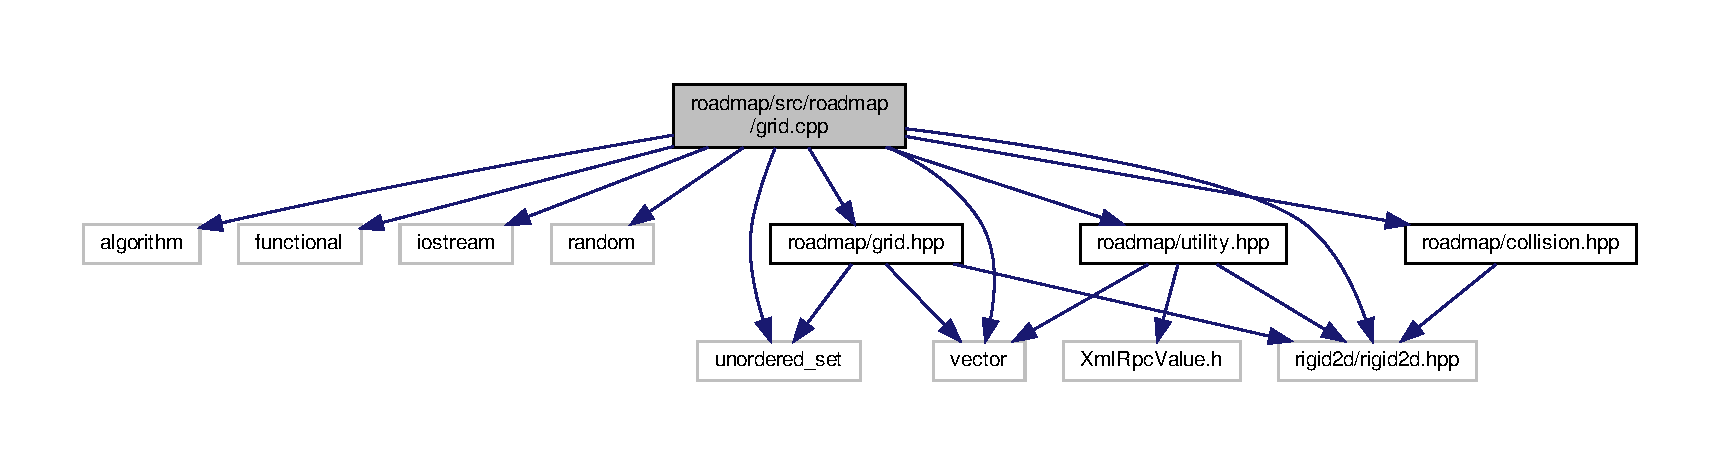
\includegraphics[width=350pt]{da/d1e/grid_8cpp__incl}
\end{center}
\end{figure}


\subsection{Detailed Description}
A library for building an occupied grid. 


\hypertarget{prm_8cpp}{}\section{roadmap/src/roadmap/prm.cpp File Reference}
\label{prm_8cpp}\index{roadmap/src/roadmap/prm.\+cpp@{roadmap/src/roadmap/prm.\+cpp}}


A library for building a Probabilistic Road Map.  


{\ttfamily \#include $<$algorithm$>$}\newline
{\ttfamily \#include $<$functional$>$}\newline
{\ttfamily \#include $<$iostream$>$}\newline
{\ttfamily \#include $<$random$>$}\newline
{\ttfamily \#include $<$unordered\+\_\+set$>$}\newline
{\ttfamily \#include $<$vector$>$}\newline
{\ttfamily \#include \char`\"{}roadmap/prm.\+hpp\char`\"{}}\newline
{\ttfamily \#include \char`\"{}roadmap/collision.\+hpp\char`\"{}}\newline
{\ttfamily \#include \char`\"{}rigid2d/rigid2d.\+hpp\char`\"{}}\newline
Include dependency graph for prm.\+cpp\+:
\nopagebreak
\begin{figure}[H]
\begin{center}
\leavevmode
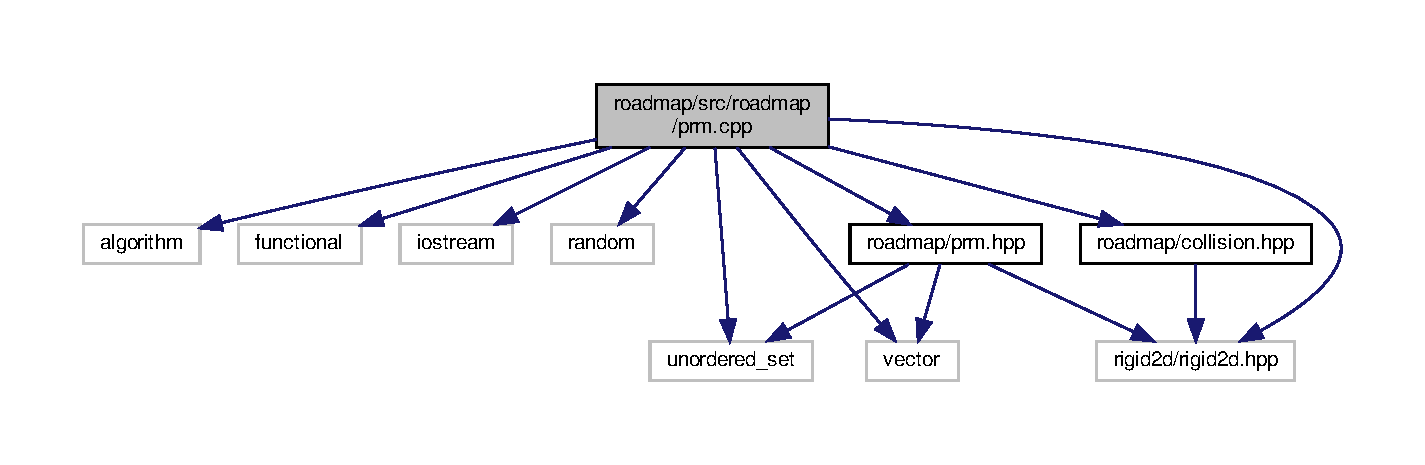
\includegraphics[width=350pt]{d9/d55/prm_8cpp__incl}
\end{center}
\end{figure}
\subsection*{Functions}
\begin{DoxyCompactItemize}
\item 
double \hyperlink{prm_8cpp_a88d1f8babd798649cc2fe9a223e48778}{prm\+::sample\+Uniform\+Distribution} (double llim, double ulim)
\begin{DoxyCompactList}\small\item\em Sample a random value between the provided limits. \end{DoxyCompactList}\end{DoxyCompactItemize}


\subsection{Detailed Description}
A library for building a Probabilistic Road Map. 



\subsection{Function Documentation}
\mbox{\Hypertarget{prm_8cpp_file_a88d1f8babd798649cc2fe9a223e48778}\label{prm_8cpp_file_a88d1f8babd798649cc2fe9a223e48778}} 
\index{prm.\+cpp@{prm.\+cpp}!sample\+Uniform\+Distribution@{sample\+Uniform\+Distribution}}
\index{sample\+Uniform\+Distribution@{sample\+Uniform\+Distribution}!prm.\+cpp@{prm.\+cpp}}
\subsubsection{\texorpdfstring{sample\+Uniform\+Distribution()}{sampleUniformDistribution()}}
{\footnotesize\ttfamily double prm\+::sample\+Uniform\+Distribution (\begin{DoxyParamCaption}\item[{double}]{llim,  }\item[{double}]{ulim }\end{DoxyParamCaption})}



Sample a random value between the provided limits. 


\begin{DoxyParams}{Parameters}
{\em llim} & the lower bound of the range \\
\hline
{\em ulim} & the upper bound of the range \\
\hline
\end{DoxyParams}
\begin{DoxyReturn}{Returns}
a random value 
\end{DoxyReturn}

%--- End generated contents ---

% Index
\backmatter
\newpage
\phantomsection
\clearemptydoublepage
\addcontentsline{toc}{chapter}{Index}
\printindex

\end{document}
